% !BIB TS-program = biber

\RequirePackage[l2tabu,orthodox]{nag}

% TODO: decide if one-sided/two-sided
\documentclass[headsepline,footsepline,footinclude=false,fontsize=11pt,paper=a4,listof=totoc,bibliography=totoc,BCOR=12mm,DIV=12]{scrbook} % two-sided
%\documentclass[headsepline,footsepline,footinclude=false,oneside,fontsize=11pt,paper=a4,listof=totoc,bibliography=totoc]{scrbook} % one-sided

% TODO: change citation style in settings
\PassOptionsToPackage{table,svgnames,dvipsnames}{xcolor}
\usepackage{enumitem}

\usepackage[utf8]{inputenc}
\usepackage[T1]{fontenc}
\usepackage[sc]{mathpazo}
\usepackage[ngerman,american]{babel}
\usepackage[autostyle]{csquotes}
\usepackage[%
  backend=biber,
  url=false,
  style=ieee,
  maxnames=4,
  minnames=3,
  maxbibnames=99,
  giveninits,
  uniquename=init]{biblatex} % TODO: adapt citation style, previously alphabetic
\usepackage{graphicx}
\usepackage{scrhack} % necessary for listings package
\usepackage{listings}
\usepackage{lstautogobble}
\usepackage{tikz}
\usepackage{pgfplots}
\usepackage{pgfplotstable}
\usepackage{booktabs}
\usepackage{amsmath}
\usepackage[final]{microtype}
\usepackage{caption}
\usepackage[printonlyused]{acronym}
\usepackage[hidelinks]{hyperref} % hidelinks removes colored boxes around references and links
\AtBeginDocument{%
	\hypersetup{
		pdftitle=\getTitle,
		pdfauthor=\getAuthor,
	}
}
\usepackage{ifthen}
\usepackage{float}

% for fachschaft_print.pdf
\makeatletter
\if@twoside
	\typeout{TUM-Dev LaTeX-Thesis-Template: twoside}
\else
	\typeout{TUM-Dev LaTeX-Thesis-Template: oneside}
\fi
\makeatother

\addto\extrasamerican{
	\def\lstnumberautorefname{Line}
	\def\chapterautorefname{Chapter}
	\def\sectionautorefname{Section}
	\def\subsectionautorefname{Subsection}
	\def\subsubsectionautorefname{Subsubsection}
}

\addto\extrasngerman{
	\def\lstnumberautorefname{Zeile}
}

% Themes
\ifthenelse{\equal{\detokenize{dark}}{\jobname}}{%
  % Dark theme
  \newcommand{\bg}{black} % background
  \newcommand{\fg}{white} % foreground
  \usepackage[pagecolor=\bg]{pagecolor}
  \color{\fg}
}{%
  % Light theme
  \newcommand{\bg}{white} % background
  \newcommand{\fg}{black} % foreground
}

\bibliography{bibliography}

\setkomafont{disposition}{\normalfont\bfseries} % use serif font for headings
\linespread{1.05} % adjust line spread for mathpazo font

% Add table of contents to PDF bookmarks
\BeforeTOCHead[toc]{{\cleardoublepage\pdfbookmark[0]{\contentsname}{toc}}}

% Define TUM corporate design colors
% Taken from http://portal.mytum.de/corporatedesign/index_print/vorlagen/index_farben
\definecolor{TUMBlue}{HTML}{0065BD}
\definecolor{TUMSecondaryBlue}{HTML}{005293}
\definecolor{TUMSecondaryBlue2}{HTML}{003359}
\definecolor{TUMBlack}{HTML}{000000}
\definecolor{TUMWhite}{HTML}{FFFFFF}
\definecolor{TUMDarkGray}{HTML}{333333}
\definecolor{TUMGray}{HTML}{808080}
\definecolor{TUMLightGray}{HTML}{CCCCC6}
\definecolor{TUMAccentGray}{HTML}{DAD7CB}
\definecolor{TUMAccentOrange}{HTML}{E37222}
\definecolor{TUMAccentGreen}{HTML}{A2AD00}
\definecolor{TUMAccentLightBlue}{HTML}{98C6EA}
\definecolor{TUMAccentBlue}{HTML}{64A0C8}

% Settings for pgfplots
\pgfplotsset{compat=newest}
\pgfplotsset{
  % For available color names, see http://www.latextemplates.com/svgnames-colors
  cycle list={TUMBlue\\TUMAccentOrange\\TUMAccentGreen\\TUMSecondaryBlue2\\TUMDarkGray\\},
}

% Settings for lstlistings
\lstset{%
  basicstyle=\ttfamily,
  columns=fullflexible,
  autogobble,
  keywordstyle=\bfseries\color{TUMBlue},
  stringstyle=\color{TUMAccentGreen},
  captionpos=b
}

% TODO: change thesis information
\newcommand*{\getUniversity}{Technische Universität München}
\newcommand*{\getFaculty}{Informatics}
\newcommand*{\getDegree}{Informatics}
\newcommand*{\getSchool}{Computation, Information and Technology}
\newcommand*{\getTitle}{Exploring Performance of B-Tree Configurations Using Machine Learning Techniques}
\newcommand*{\getTitleGer}{Untersuchung der Performance von B-Baum-Konfigurationen durch Techniken des maschinellen Lernens}
\newcommand*{\getAuthor}{Roland Haidari}
\newcommand*{\getDoctype}{Bachelor's Thesis}
\newcommand*{\getSupervisor}{Prof. Dr. Viktor Leis}
\newcommand*{\getAdvisor}{M.Sc. Marcus Müller}
\newcommand*{\getSubmissionDate}{15.03.2024}
\newcommand*{\getSubmissionLocation}{Garching}

\begin{document}

% Set page numbering to avoid "destination with the same identifier has been already used" warning for cover page.
% (see https://en.wikibooks.org/wiki/LaTeX/Hyperlinks#Problems_with_Links_and_Pages).
\pagenumbering{alph}
\begin{titlepage}
  % HACK for two-sided documents: ignore binding correction for cover page.
  % Adapted from Markus Kohm's KOMA-Script titlepage=firstiscover handling.
  % See http://mirrors.ctan.org/macros/latex/contrib/koma-script/scrkernel-title.dtx,
  % \maketitle macro.
  \oddsidemargin=\evensidemargin\relax
  \textwidth=\dimexpr\paperwidth-2\evensidemargin-2in\relax
  \hsize=\textwidth\relax

  \centering

  \IfFileExists{logos/tum-logo.png}{%
    \includegraphics[height=20mm]{logos/tum-logo.png}
  }{%
    \vspace*{20mm}
  }

  \vspace{5mm}
  {\huge\MakeUppercase{School of \getSchool{} --- \getFaculty{}} \par}

  \vspace{5mm}
  {\large\MakeUppercase{\getUniversity{}} \par}

  \vspace{15mm}
  {\Large \getDoctype{} in \getDegree{} \par}

  \vspace{10mm}
  {\huge\bfseries \getTitle{} \par}

  \vspace{10mm}
  {\LARGE \getAuthor{}}

  \IfFileExists{logos/faculty-\fg.pdf}{%
    \vfill{}
    \includegraphics[height=20mm]{logos/faculty-\fg.pdf}
  }{}
\end{titlepage}


\frontmatter{}

\begin{titlepage}
  \centering

  \IfFileExists{logos/tum-logo.png}{%
    \includegraphics[height=20mm]{logos/tum-logo.png}
  }{%
    \vspace*{20mm}
  }

  \vspace{5mm}
  {\huge\MakeUppercase{School of \getSchool{} --- \getFaculty{}} \par}

  \vspace{5mm}
  {\large\MakeUppercase{\getUniversity{}} \par}

  \vspace{20mm}
  {\Large \getDoctype{} in \getDegree{} \par}

  \vspace{15mm}
  {\huge\bfseries \getTitle{} \par}

  \vspace{10mm}
  {\huge\bfseries \foreignlanguage{ngerman}{\getTitleGer{}} \par}

  \vspace{15mm}
  \begin{tabular}{l l}
    Author:          & \getAuthor{}         \\
    Supervisor:      & \getSupervisor{}     \\
    Advisor:         & \getAdvisor{}        \\
    Submission Date: & \getSubmissionDate{} \\
  \end{tabular}

  \IfFileExists{logos/faculty-\fg.pdf}{%
    \vfill{}
    \includegraphics[height=20mm]{logos/faculty-\fg.pdf}
  }{}
\end{titlepage}

\thispagestyle{empty}
\vspace*{0.8\textheight}
\noindent
I confirm that this \MakeLowercase{\getDoctype{}} is my own work and I have documented all sources and material used.

\vspace{15mm}
\noindent
\getSubmissionLocation{}, \getSubmissionDate{} \hspace{\fill} \getAuthor{}

\cleardoublepage{}

%\addcontentsline{toc}{chapter}{Acknowledgments}
\thispagestyle{empty}

\vspace*{20mm}

\begin{center}
    {\usekomafont{sectioning}\usekomafont{section} Acknowledgments}
\end{center}

\vspace{10mm}

%TODO: Acknowledgments

\cleardoublepage{}

\chapter{\abstractname}

This thesis aims to identify potential improvements for B+ tree implementations using \ac{XAI} on \ac{ML} models. It starts by generating a dataset using the \ac{ycsb} benchmark, preprocessing the results, training \ac{ML} models, and finally analyzing the results of \ac{XAI} algorithms. Through this process, the thesis delves into various stages of the data science life cycle. Additionally, pattern recognition algorithms, Apriori and association rules, are described and used, which further verify some insights found by the \ac{XAI} approach.
\\\\
Building on the work of Müller et al. \parencite{mueller2024} the findings of this thesis contribute to our understanding of B+ trees by highlighting the impact of data skewness, size of values, number of records and the page size of leaf nodes on the performance. Beyond the domain of B+ trees, this thesis, concludes that the currently available \ac{XAI} algorithms can be utilized to enhance the interpretability of outputs originating from \ac{ML} models.   



\microtypesetup{protrusion=false}
\tableofcontents{}
\microtypesetup{protrusion=true}

\mainmatter{}

\chapter{Introduction}\label{chapter:introduction}

In computer systems, good responsiveness of systems is desired to achieve fast retrieval of information. Where and how data is stored, can greatly impact the latency of data storage systems. Traditionally, systems would offload data to disk, which would lead to slower performance. More modern hardware technologies allow storing bigger amounts of data in-memory, which brings lower latency. To optimize storage, there exist numerous data structures and ways to store the data. One important factor, however, is the need to be able to efficiently offload data to secondary storage, once the memory limits are reached. 
\\\\
The B+ tree structure enabled managing data in-memory and supports disk storage as well. In their paper, Müller et al. \parencite{mueller2024} aim to optimize the performance of B+ trees by exploring various possible configurations and optimizations on different datasets and statistically analyzing the performance impacts of the configurations. 
\\\\
Nowadays, according to Davenport \parencite{FiveKeyT68:online}, \ac{ML} and Artificial Intelligence has taken more relevance in the data science world. The idea of gaining insights with smart algorithms and large amounts of data is naturally intriguing. This thesis attempts to utilize machine learning to find potential optimization techniques of B+ trees. To do so, multiple steps need to be taken. These steps, as explained by Stodden in \parencite{datasciencelifecycle}, include data collection, data exploration, data preprocessing, model training and model evaluation. Together these steps form the data science life cycle.
\\\\
Once a well-performing model is trained, it can be attempted to analyze and explain the insights that the \ac{ML} model has learned. \ac{XAI} is a field in the data science that focuses on this idea. This thesis, tries to apply common \ac{XAI} techniques to the trained models to verify existing insights or gain new - possibly unseen - information that could help optimize B+ tree performance.
\\\\
In addition to the classical model training and \ac{XAI}, a data-mining pattern recognition approach is taken, where two algorithms are used to gain insights by computing frequent itemsets and association rules.
\\\\
The code base, excluding the datasets, is published in the GitHub repository at \url{https://github.com/rolandhaidari/thesis}.
\chapter{B+ Tree Implementations}\label{chapter:b-tree_implementations}
\section{B+ Tree}
\subsection{Structure}
The original paper on B-Trees \parencite{ogbtree} describes a data structure, where data is managed in a tree-like structure, with a node containing data, and having children with one node being on top, called the root. According to Graefe \parencite{modernbtree} it has self-balanced mechanisms that ensure that the data is remained sorted and lookups require an efficient amount of comparisons by the utilizing binary sort techniques. In Figure \ref{fig:btreeexample} the root node contains three values and references the children in a sorted manner.
\begin{figure}[h]
  \centering
  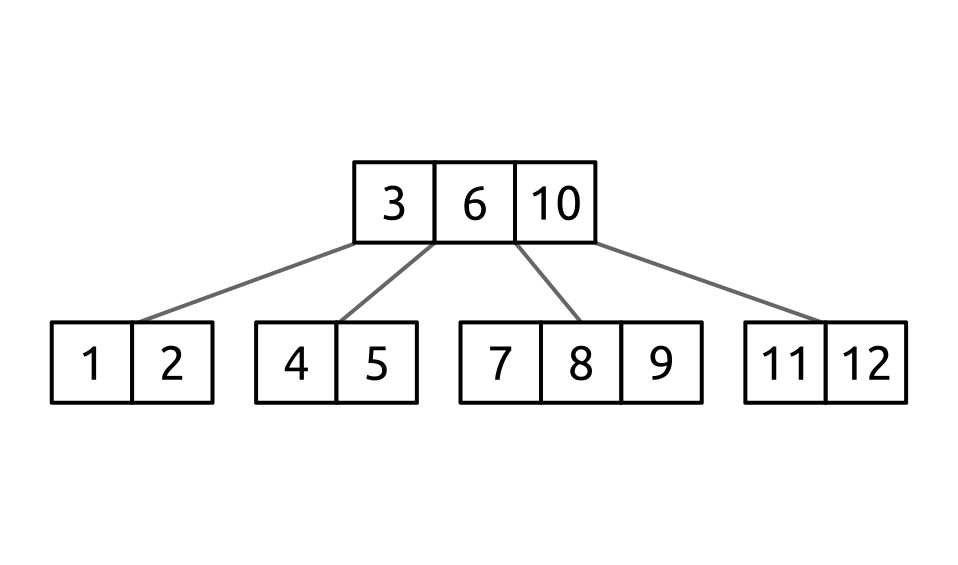
\includegraphics[width=0.5\textwidth]{images/an-example-b-tree.png}
  \caption{Simple B-Tree example \parencite{btreeexample}}
  \label{fig:btreeexample}
\end{figure}
\\\\
Graefe \parencite{modernbtree} further discusses that B+ tree is a variant of the B-tree. Instead of storing the values inside the all nodes it stores the values in the lowest layer, called the leaf nodes. The inner nodes keep track of the keys and reference child nodes, in a sorted manner. To be able to traverse key ranges fast, the leaf nodes can contain a reference to the neighboring leaf node. The implementation by Müller et al. \parencite{mueller2024} does not implement these references. The figure \ref{fig:b+treeexample} outlines a simple example of this variation. The data is structured by keys and values. For example, the number $3$ represents the key $3$ and the middle leaf node contains the reference to the corresponding value $d_3$. In this figure, the references to neighboring leaf nodes are visualized in dark red.


\begin{figure}[h]
  \centering
  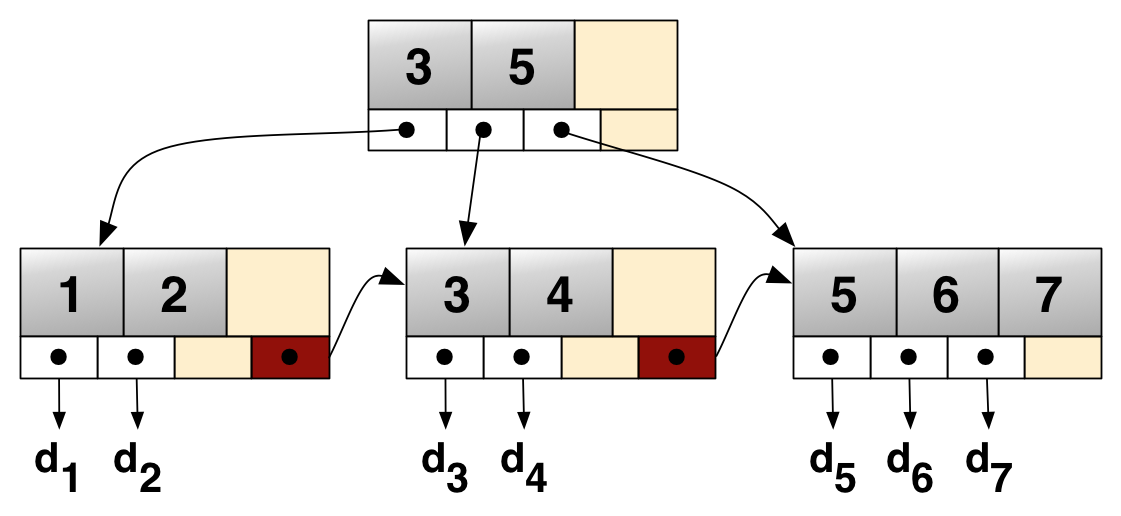
\includegraphics[width=0.5\textwidth]{images/Bplustree.png}
  \caption{Simple B+ tree example \parencite{wikib+tree}}
  \label{fig:b+treeexample}
\end{figure}
 
\subsection{Operations}
The B+ tree, similarly to the B-tree, has, among others, the following operations: Insertion, Search, Deletion, and Range Queries. The differences between the B+ tree and the B-tree lie in the nature of the structures, and therefore the operations have differences in memory usage and performance. Some operations are more suited in a B+ tree than a B-tree. The table \ref{fig:operationstable} outlines the differences in regard to the operations. Overall, a notable downside of B+ trees is the generally bigger storage use, since a B-tree is able to store values in the inner nodes. Graefe \parencite{modernbtree} reported that this downside, however, simplifies some operations, bringing an overall, better performance, making the B+ tree the default structure in modern times. This thesis focuses on the B+ tree and the operations of insertion and range querying. 
\\\\
In this thesis, we consider the operations described in by Müller et al. \parencite{mueller2024}, namely \textbf{insert, remove, lookup, scan} and more specifically the \textbf{insert}, \textbf{lookup} and \textbf{scan} operations.

\begin{table}[htbp]
\centering

\begin{tabular}{|p{2cm}|p{3cm}|p{4cm}|p{4cm}|}
\hline
\textbf{Operation} & \textbf{Description} & \textbf{B-tree} & \textbf{B+ tree} \\
\hline
Search (\textbf{lookup}) & Finding a given key in the tree. & Binary search through the tree & Same as B-tree. \\
\hline
Insertion (\textbf{insert}) & Adding a key-value pair & Values are also stored in internal nodes. & Keys are stored in internal nodes, Values only in leaf nodes. \\
\hline
Deletion (\textbf{remove}) & Removing a key-value pair & Since values are stored in the internal nodes, merging and redistribution operations are more complex. & Simplified merging and redistribution. \\
\hline
Range Queries (\textbf{scan}) & Retrieving a range of keys or values & Less suitable due to values stored in internal nodes. & More suitable because of leaf nodes containing pointers to their succeeding leaf node, which allows sequential access. \\
\hline
Traversal & Iterating through all keys or values in sorted order. & Follows a dept-first approach. & Reduced complexity, since values are only in linked leaf nodes, only requiring one big range query.  \\
\hline
Splitting Nodes & Full nodes are divided into two nodes. & May redistribute keys and values. & Only internal nodes (keys) are affected. Values are not redistributed.  \\
\hline
Merging Nodes & During deletion, nodes may become too empty. Nodes need to be merged as a consequence. & Keys and values need to be redistributed & Simplified as only keys are affected. \\
\hline
\end{tabular}
\caption{Comparison of Operations in B-trees and B+trees}
\label{fig:operationstable}
\end{table}



\section{Optimizations}

The paper by Müller et al. \parencite{mueller2024} uses an implementation of the B+ tree that is implemented in the programming language C++. The paper outlines certain optimizations and configurations that can be utilized with the aim to improve operation runtime performance. The following optimizations have been proposed: 

\begin{itemize}
  \item \textbf{Prefix Truncation} refers to truncating the prefixes that are shared among keys stores in a node. An example for such truncation is cutting off the prefix "\textit{https://}" in url data. This brings benefits to storage use and the cache is better utilized. The key transfer between nodes requires an extra operation, which adds complexity, however as this operation is rare, the runtime cost is minimal. 
  
  \item \textbf{Heads} is the idea of taking the first 4 bytes of the key, named \textit{head}, and using those for the binary search. This enables better use of the cache. The figure \ref{fig:heads} represents this idea by using the first letter of the keys as heads. On the other hand, the slots with heads would require more bytes to be aligned. The implementation by Müller et al. \parencite{mueller2024} decided on doing unaligned access, since the negative impact is believed to be negligible. \\
  
  \begin{figure}[h]
      \centering
      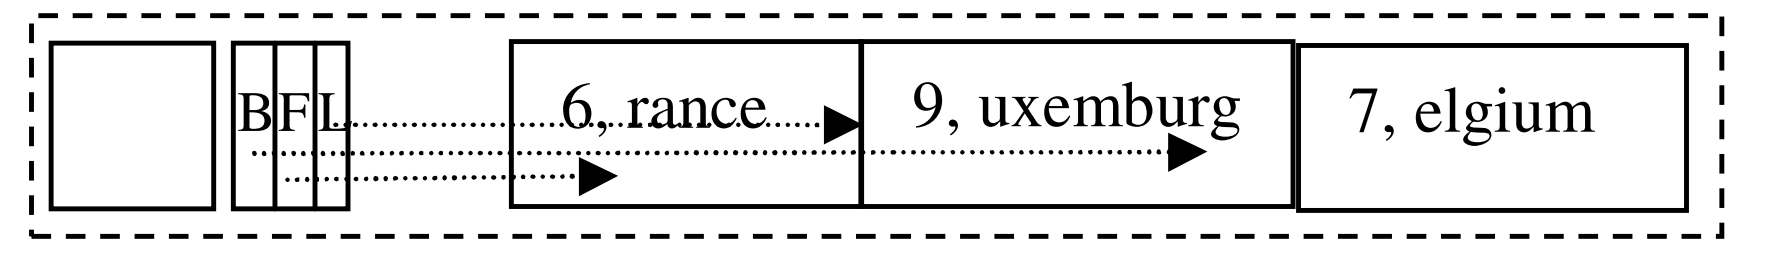
\includegraphics[width=0.5\textwidth]{images/heads.png}
      \caption{Heads example \parencite{modernbtree}}
      \label{fig:heads}
  \end{figure}
    
  \item \textbf{Hints} takes the idea of \textbf{heads} one step further, by adding a structure called hint array to each node header. The array contains the heads of equidistant slots, as visualized in figure \ref{fig:hints}. The implementation by Müller et al. \parencite{mueller2024} sets the hint array to the size of 16 hints, and the array is updated only at or after the insertion. 

  \begin{figure}[h]
      \centering
      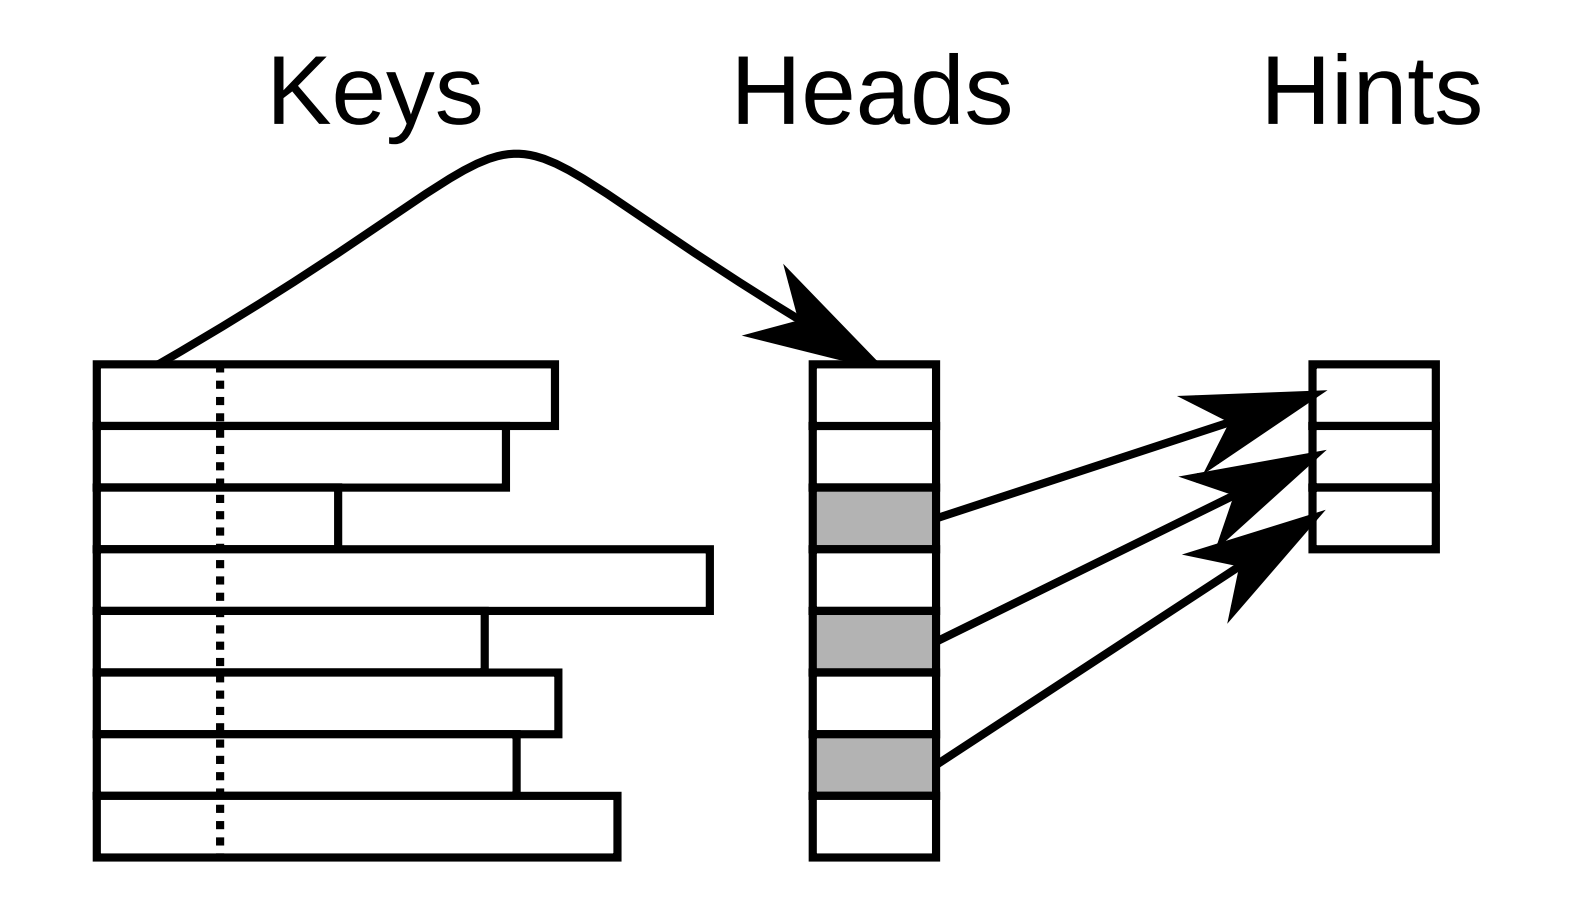
\includegraphics[width=0.5\textwidth]{images/hints.png}
      \caption{Hints from heads \parencite{mueller2024}}
      \label{fig:hints}
  \end{figure}
    
  \item \textbf{Fingerprinting} introduces an array of key hashes in the heap of the node. The figure \ref{fig:hash} is an example for such an array. The array contains a sorted and an unsorted part. During insertion, the values are appended to the end - the unsorted part. The fingerprint array only gets sorting during scan, node splitting, merging operations. If used in combination with \textbf{prefix truncation}, the prefixes get truncated before calculating the hash. Additionally, to improve performance of search operations on nodes the SIMD instructions with a range of 256 bit are used.
  
  \begin{figure}[h]
      \centering
      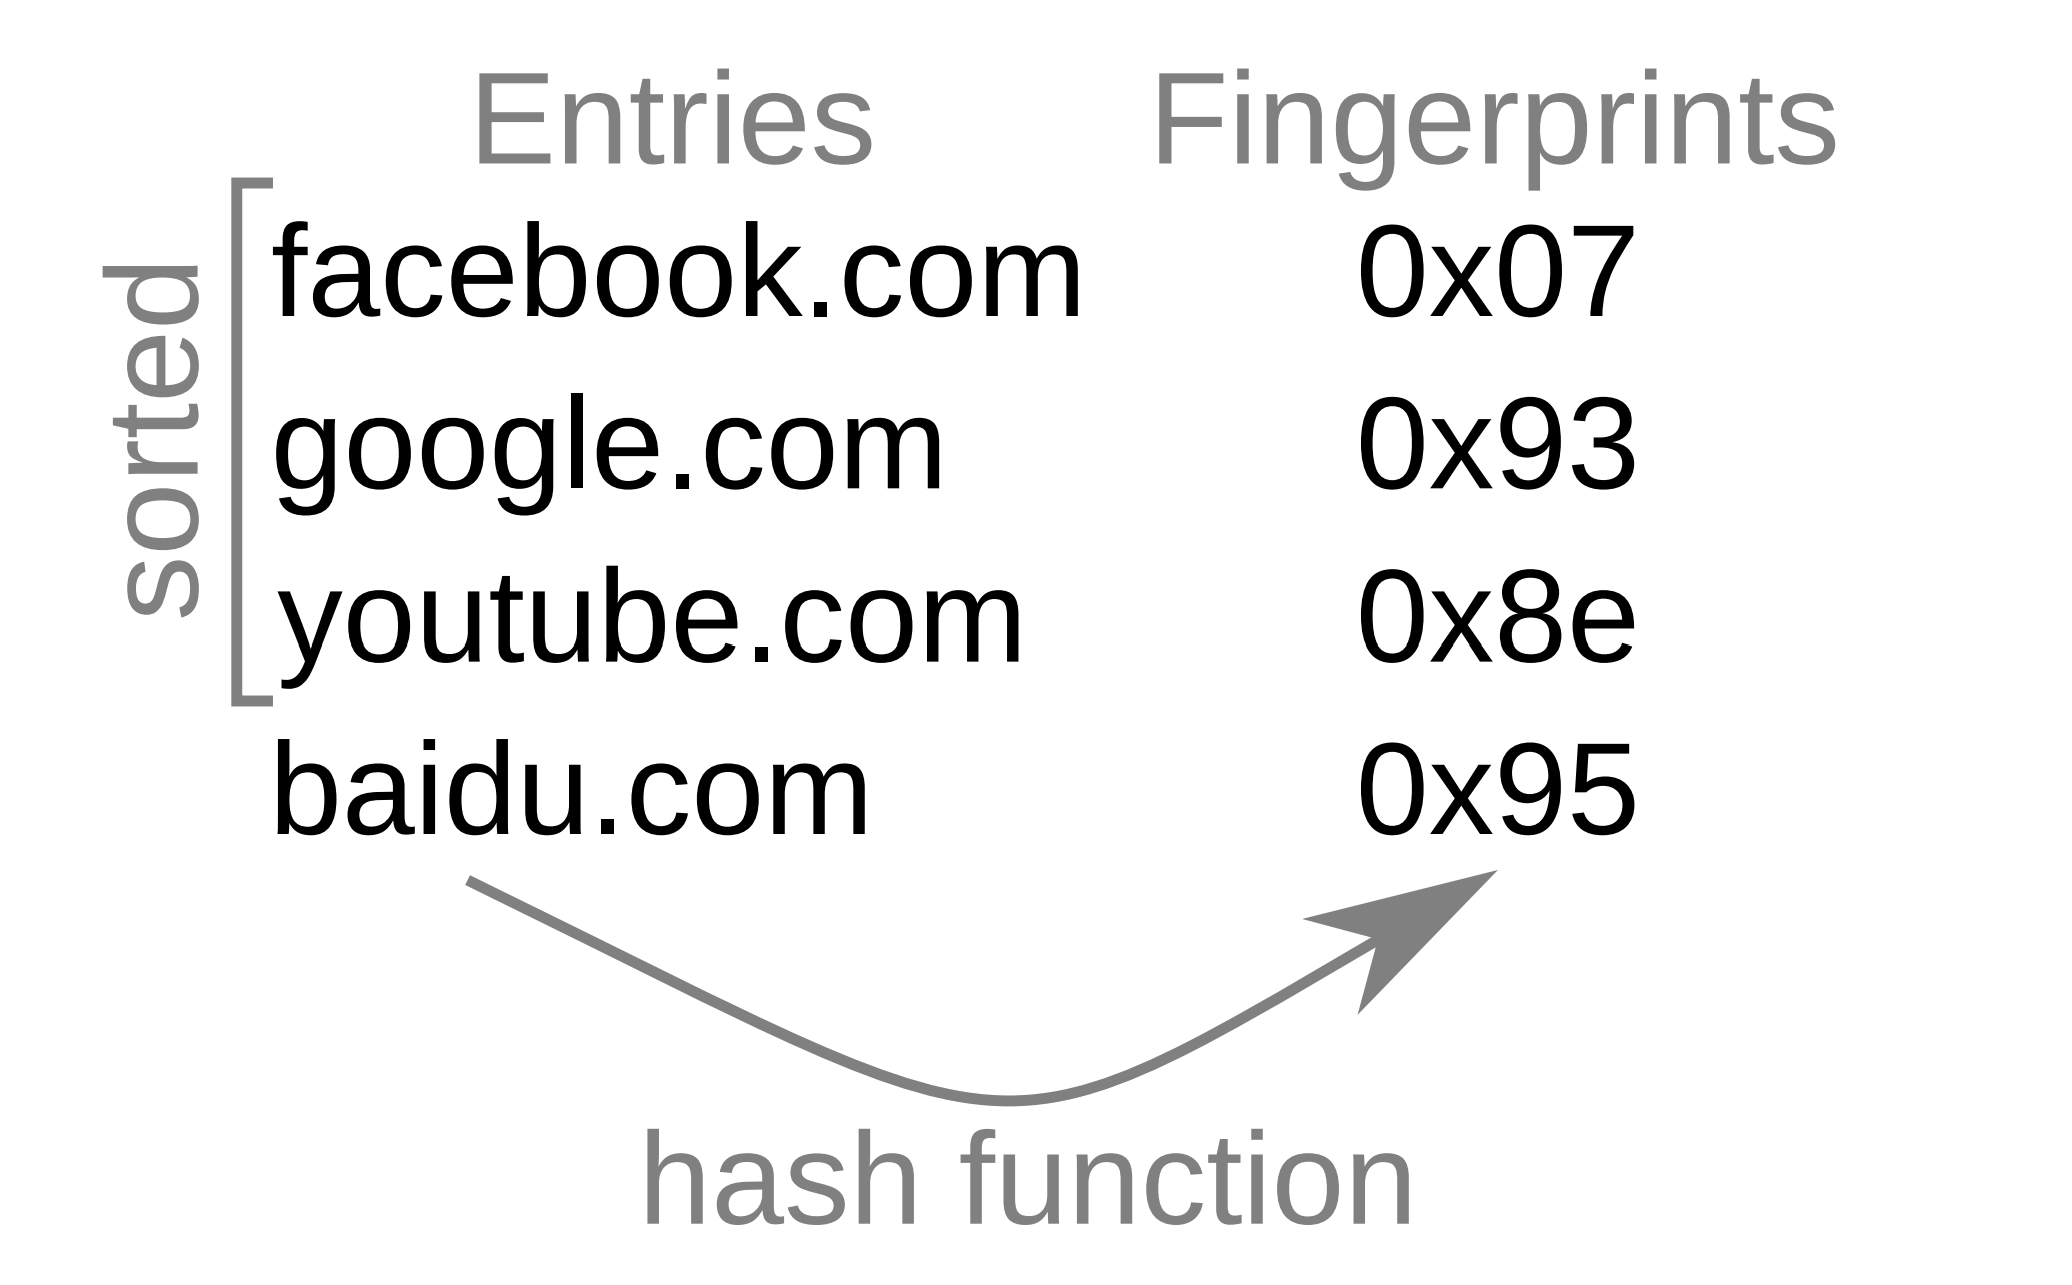
\includegraphics[width=0.5\textwidth]{images/hash.png}
      \caption{Fingerprinting array \parencite{mueller2024}}
      \label{fig:hash}
  \end{figure}
    
  \item \textbf{Dense Leaves} is a new approach introduced by Müller at al. \parencite{mueller2024}, based on the idea of using frame-of-reference encoding to keys. Frame-of-reference encoding takes reference keys and calculates the offsets for the following values. This idea is meant for keys that are dense enough, thereby mitigating the inefficiency associated with underutilized storage space. Two approaches are presented, namely \textbf{Semi Dense Leaves} and \textbf{Fully Dense Leaves}. As presented in figure \ref{fig:denseLeaves}, Semi Dense Leaves contain pointers at each possible offset to the node's heap containing the keys and values. The Fully Dense Leaves implementation presumes that the values are of the same size, which is a common characteristic for specific types of data. Additionally, a partition mechanism is implemented, which recognizes dense keys originating from different sources and therefore ensuring that the tree stores data more densely.

  \begin{figure}[h]
      \centering
      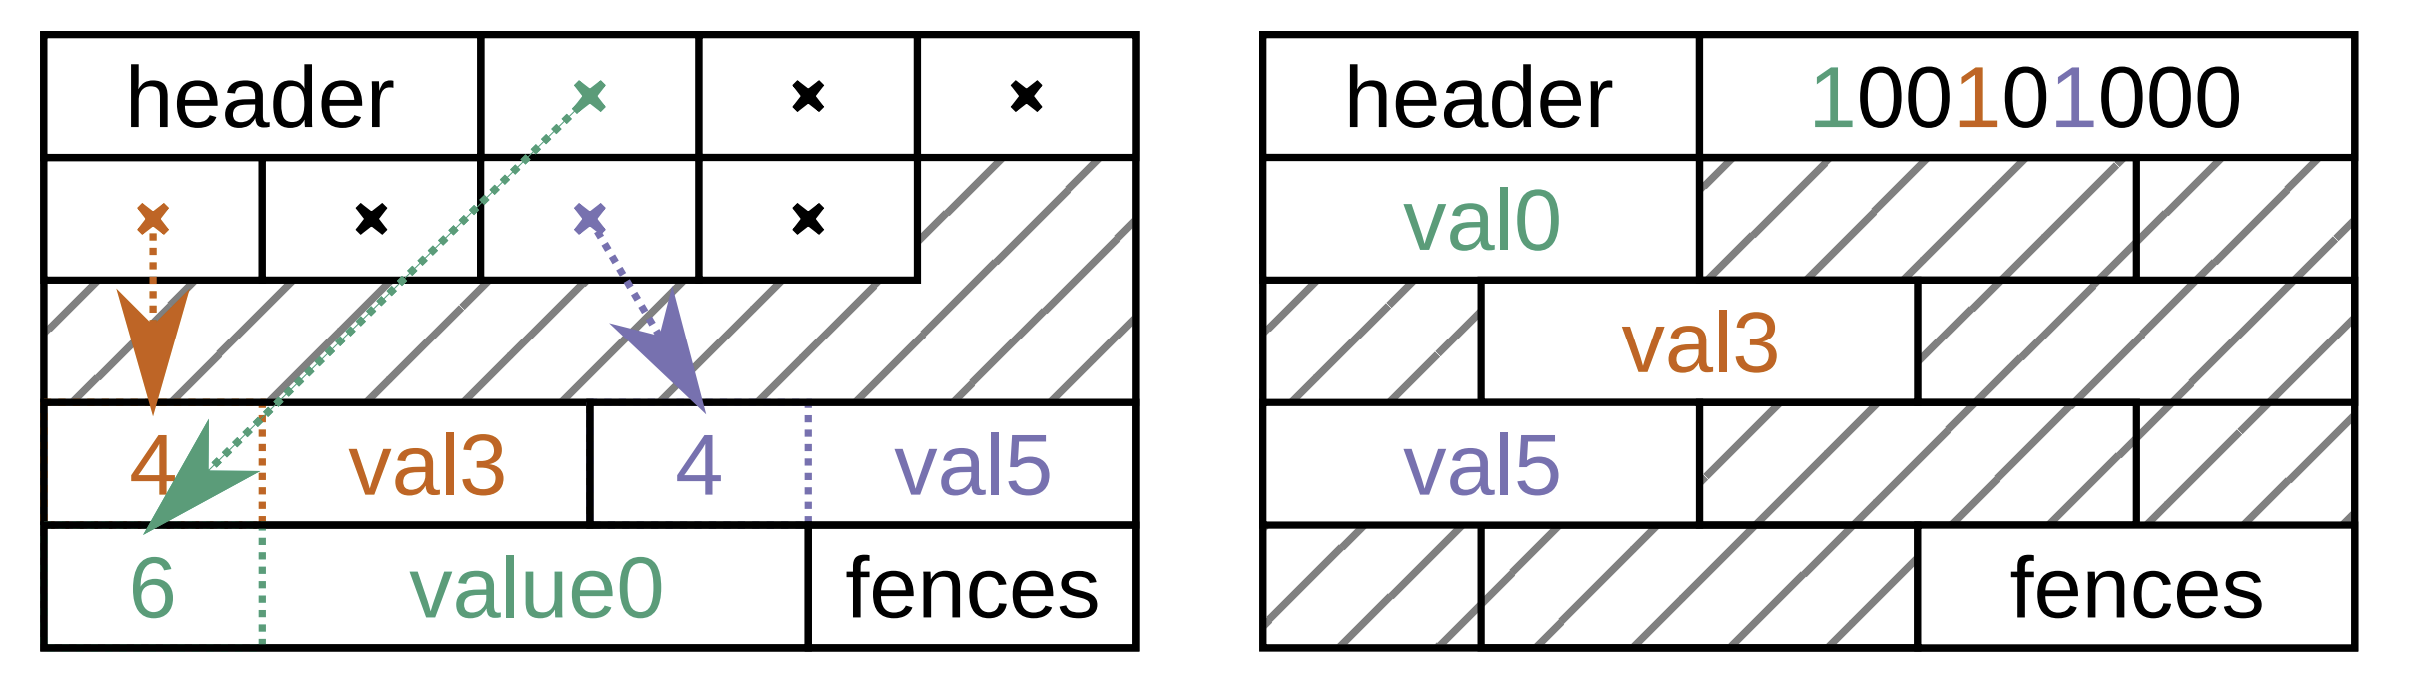
\includegraphics[width=0.5\textwidth]{images/denseLeaves.png}
      \caption{Example of Semi (left) and Fully (right) Dense Leaves with three values \parencite{mueller2024}}
      \label{fig:denseLeaves}
  \end{figure}
     
\end{itemize}

\section{Adaptable B+ tree}
Müller et al. \parencite{mueller2024} further discusses the topic of creating a B+ tree, which is adaptable, meaning that it can adjust the type of leafs to circumstances and the type operations. One approach is proposed, and shows considerable performance improvements in its benchmarks. The figure \ref{fig:adapt} describes, in which circumstances, leafs are transitioned into a different type.
  \begin{figure}[h]
      \centering
      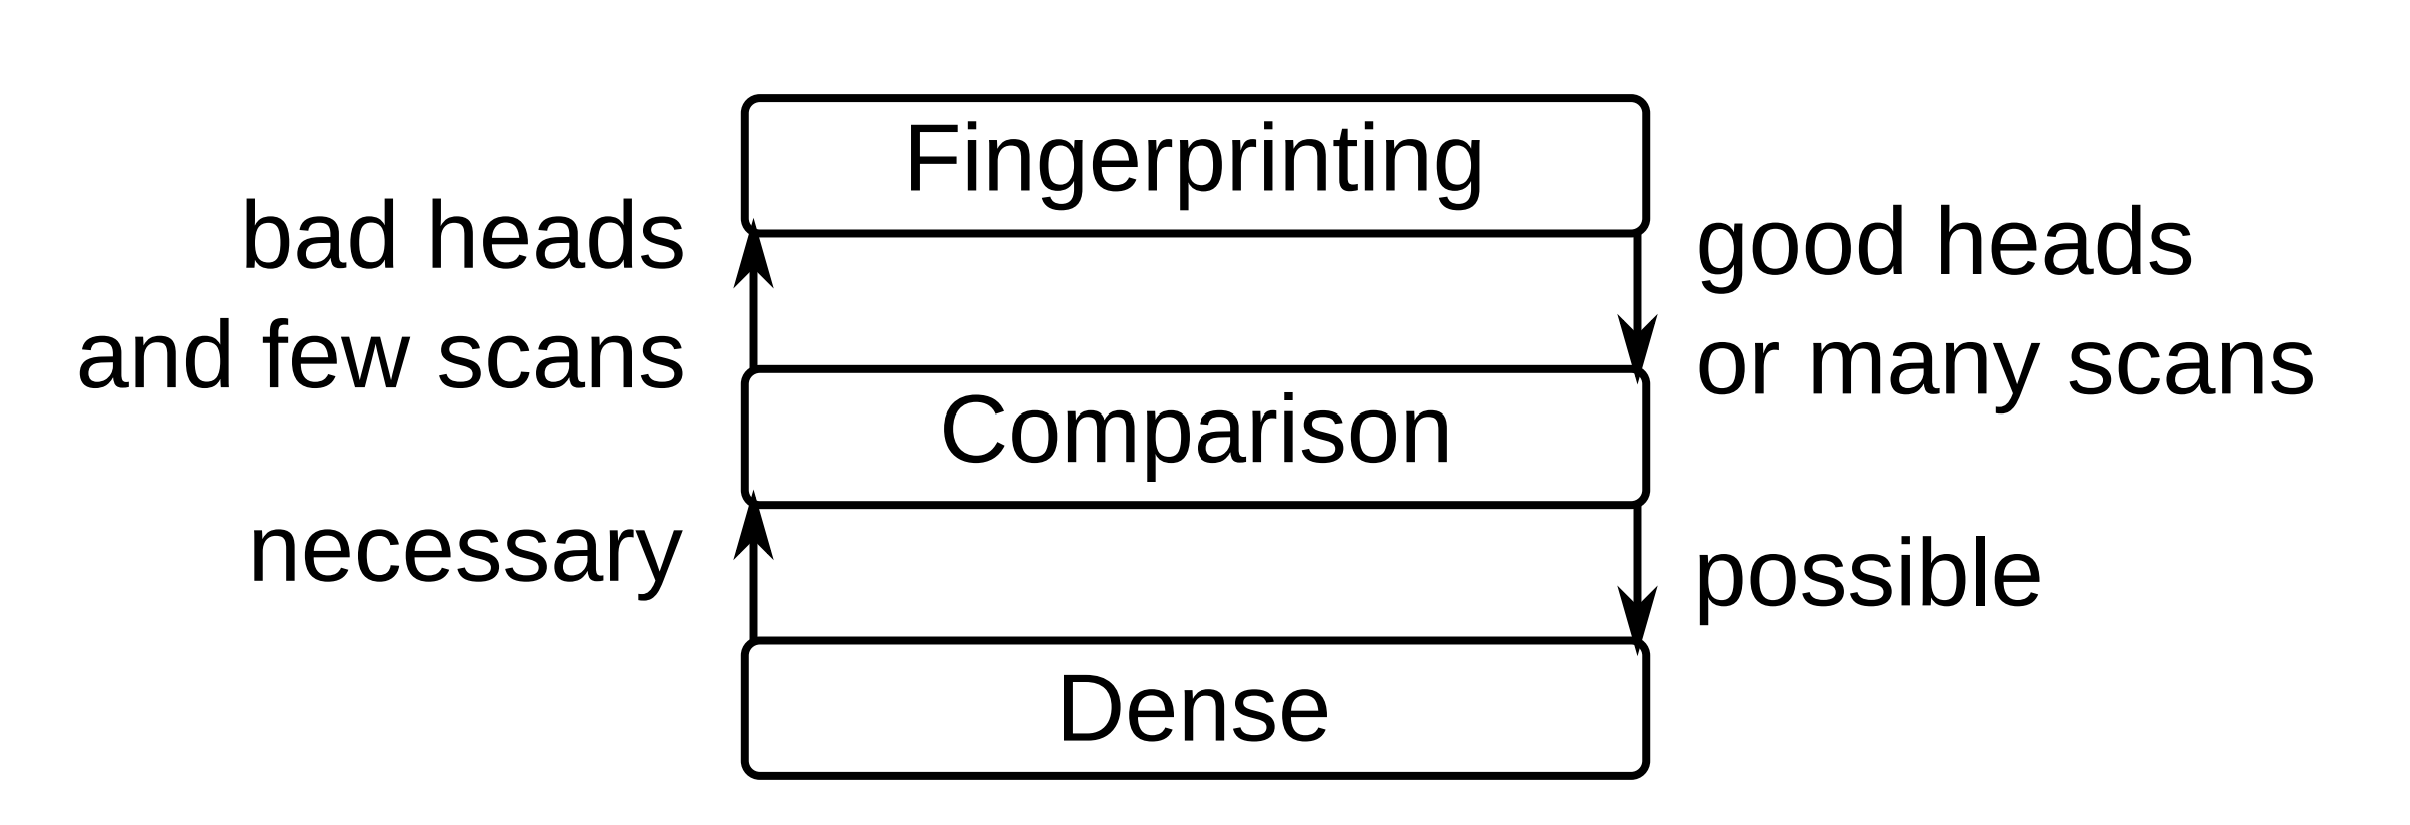
\includegraphics[width=0.5\textwidth]{images/adapt.png}
      \caption{Decisions on leaf layout \parencite{mueller2024}}
      \label{fig:adapt}
  \end{figure}
\\\\
This thesis takes this idea and aims to get more insights into the possible approaches of configuring B+ trees. The goal is to improve on the idea of adaptable B+ trees, by finding factors impacting the performance in various configuration combinations. Particularly, the focus lies on the page size of leaf nodes, since this configuration is easily adaptable during runtime. 
%\chapter{Development Environment}\label{chapter:environment}
Introduction about why I set up the way I did and that Structuring Data is useful. Mention that in a organisation more automated tools would be used. Since this is data exploration, it is not. \\
Mention data generated on server, results copied to local device, where it is analyzed. \\

\subsection{Version Control}
Rougly describe Git and why it is used
\subsection{Tools}
Python, Poetry, Jupyter, VSCode

\subsection{Folder structure}
Separated into following sections:\\
- Generate data\\
- Binaries\\
- Data\\
- Output\\
- Data Science\\
-- Preprocessing\\
-- Analysis\\
-- CNN\\
-- Regression\\
-- Classification\\ 
-- XAI\\
-- pattern recognition\\


\subsection{Libraries used}
Name them in a list and describe where they were used
pandas\\
seaborn \\
matplotlib\\ 
scikit-learn\\
shap \\
interpret\\ 
lime \\
statsmodels \\ 
mlxtend \\
\chapter{Preprocessing}\label{chapter:preprocessing}
This chapter describes, how the data has been collected and what steps have been done to transform the data, so that it is suitable for training models.

\section{Data collection}
\subsection{Environment}
During creating benchmarking data, it is necessary to create the same conditions, at each run of the program. Preferably, the data generation occurs on dedicated machines, where little to no other background processes can impact the performance of the benchmarking program. This approach has been taken in this thesis, where the data generation, occurs only at times, where no other user is using the same machine concurrently. This was ensured, by registering who uses the machine at a table on a shared tabular scheduling sheet. The table \ref{tab:system_info} describes the hardware and software characteristics of the server machine running the data generation program. 

\begin{table}[h]
\centering
\begin{tabular}{|l|l|}
\hline
\textbf{Characteristic} & \textbf{Value} \\ \hline
CPU Product & AMD Ryzen 9 7950X 16-Core Processor \\ \hline
CPU Vendor & Advanced Micro Devices [AMD] \\ \hline
CPU Cores & 16 \\ \hline
CPU MHz & 3360.195 \\ \hline
Total Memory & 64 GB \\ \hline
OS Description & Ubuntu 23.10 \\ \hline
Architecture & x86\_64 \\ \hline
Linux Kernel version & 6.5.0-15-generic \\ \hline
\end{tabular}
\caption{Benchmarking Server System Information}
\label{tab:system_info}
\end{table}

\subsection{Binary programs}
After making sure that the data can be collected consistently, the subsequent phase involves thinking about how the data is to be collected. For the purpose of this thesis, program binaries have been provided, which execute the B+ tree configuration behavior as defined by Müller et al. \parencite{mueller2024}. Each binary file executes a b-tree configuration using the inputs and 
produce output a multi-line string in the comma-separated format containing input configuration together with the measured outputs. More details on the operations being benchmarked are provided in section \ref{subsec:ycsb}.
The input and the output values are further outlined in feature tables, table \ref{tab:input_features_example} and table \ref{tab:output_features_example}. In the feature tables, for numerical and boolean features, if only one value is provided as an example, this feature is not varied in further context. 
\\\\
Each run of a single binary gives an output in three lines. The first line describes the header of the comma-separated values. The second and third contain the inputs and output in the comma-separated format of the initialization of the operation and the actual operation, respectively.
\\\\
When calling a binary program, some of the input parameters are embedded in the binary itself, in which case changing it requires a call to a different binary. This is the case for the inner and leaf node page size and the configuration (eg. hints, head). The rest of the parameters are passed to the binary program by setting environment variables beforehand. 
\begin{table}[H]
\centering
\resizebox{\textwidth}{!}{
\begin{tabular}{|l|l|l|}
\hline
\textbf{Feature} & \textbf{Description} & \textbf{Example Value(s)} \\ \hline
bin\_name & Name of the binary & \texttt{bins/-DPS\_I=4096 -DPS\_L=4096/hints-n3-ycsb} \\ \hline
config\_name & set of optimizations &  hash, hints, baseline, prefix, dense3\\ \hline
const\_basicHintCount & Basic hint count & 16 , 0 \\ \hline
const\_enableBasicHead & Enable basic head optimization& 1 \\ \hline
const\_enableDense & Enable dense optimization& 0 , 1 \\ \hline
const\_enableDense2 & Enable dense 2 optimization& 0 \\ \hline
const\_enableDensifySplit & Enable densify split & 0 , 1 \\ \hline
const\_enableHash & Enable hash optimization & 0 , 1 \\ \hline
const\_enableHashAdapt & Enable adapation optimization & 0 \\ \hline
const\_enableHeadNode & Enable head node optimization& 0 \\ \hline
const\_enablePrefix & Enable prefix truncation optimization & 1 \\ \hline
const\_hashSimdWidth & SIMD operation width & 32 \\ \hline
const\_hashSortUseStdMerge & Hash sort use standard merge & 1 \\ \hline
const\_hashUseCrc32 & Hash use CRC32 & 0 \\ \hline
const\_hashUseSimd & Hash use SIMD & 1 \\ \hline
const\_headNode4HintCount & Head node 4 hint count & 16 \\ \hline
const\_headNode8HintCount & Head node 8 hint count & 16 \\ \hline
const\_pageSizeInner & Inner node page size & 2048, 4096, 8192 \\ \hline
const\_pageSizeLeaf & Leaf node page size & 2048, 4096, 8192 \\ \hline
data\_name & Name of the data & data/urls, int \\ \hline
data\_size & Size of the data, key count &  5181932, 2813666\\ \hline
data\_sorted & Data sorted status & 0 \\ \hline
density & Density & 0.5, 0.75, 1 \\ \hline
op & Operation & ycsb\_c, ycsb\_c\_init, ycsb\_e, ycsb\_e\_init \\ \hline
payload\_size & Size of values & 8, 256 \\ \hline
rand\_seed & Random seed & 1703378455, 1703378098 \\ \hline
run\_id & Run ID & fc16dbaa-104b-4777-8087-bbe953b81b16 \\ \hline
ycsb\_range\_len & YCSB range length & 100 \\ \hline
ycsb\_zipf & YCSB zipf & 0.9, 0.651367 \\ \hline
\end{tabular}
}
\caption{Input Features with Example Values}
\label{tab:input_features_example}
\end{table}



\begin{table}[H]
\centering
\resizebox{\textwidth}{!}{
\begin{tabular}{|l|l|l|}
\hline
\textbf{Feature} & \textbf{Description} & \textbf{Example Value(s)} \\ \hline
time & Time in seconds &  1.0512e-06, 3.126e-07 \\ \hline
nodeCount\_X & Node count of type X & 19755, 20879 \\ \hline
counted\_final\_key\_count & Final key count & 5798920, 3175985 \\ \hline
cycle & Average number of CPU cycles pro operation & 2197.381, 1087.615 \\ \hline
instr & Average CPU instructions pro operation & 1927.571 1151.517 \\ \hline
X\_miss & Average misses pro operation in cache type X  & 43.867, 9.918  \\ \hline
task & Kernel execution time & 392.291, 194.439 \\ \hline
scale & Scale &  5798920, 10000000 \\ \hline
IPC & Instructions Per Cycle & 0.877, 1.059 \\ \hline
CPU & CPU usage & 1, 0.993, 0.99 \\ \hline
GHz & CPU frequency & 5.601, 5.594 \\ \hline
\end{tabular}
}
\caption{Output Features with Example Values}
\label{tab:output_features_example}
\end{table}


\subsection{Data generation program}

Collecting the data is done through a Python script that runs in a loop, that terminates after a configured timeout. Inside the loop, the input parameters are generated either with a constant, or depending on the use case randomly from a given set, or a random value in a range. The outputs are collected and appended to three different files: the error logging file, the output file and the logging of the script file. Each file serves a purpose. The error logging file is useful to identify issues with the binaries that are called. The output file contains the data that is later analyzed. The logging of the script file is useful to identify issues of the Python script itself. \\ \\
Two versions of this script exist that set the generation of the input parameters for the specific use case. For general model building more values are generated at random, whereas for the analysis of the page size, the values are more fixed to be able to be able to better make use of discrete data mining algorithms.\\ \\
The Python script is called in a Poetry \parencite{poetry:online} environment and to make the script run in the background the \textit{nohup} \parencite{nohup1Li95:online} command is utilized.\\ \\
Once the script is finished running, the output files are checked to verify a successful run. Since the following steps do not require a consistent environment, the output files are copied to a local device, where the output is further processed, analyzed and other experiments are run.

\subsubsection{ML model program}
For the use case of training the \ac{ML} models, the input parameters are set to the following values:

\begin{itemize}
    \item \textbf{ycsb\_zipf}: Random value between 0 and 1.5 
    \item \textbf{op}: The operations \textit{c} with \textit{c\_init} are chosen twice as much as \textit{e} with \textit{e\_init} 

    \item \textbf{data\_name}: Set statically to \textit{data/urls}

    \item \textbf{const\_pageSizeLeaf}: Randomly varied in powers of two between 2048 and 16384 
    \item \textbf{const\_pageSizeInner}: Randomly varied in powers of two between 2048 and 16384 
    \item \textbf{payload\_size}: Set statically to 8
    \item \textbf{density}: Generated with \texttt{ 1 / 2 ** random()}
    \item \textbf{config\_name}: Randomly chosen between \textit{dense3}, \textit{hints} and \textit{hash}
    \item \textbf{data\_size}: Generated by \texttt{ floor((10 ** (random() * 0.5 + 8.25))/ 70.280)}. \texttt{70.280} corresponds to an estimated average size of a key.  
\end{itemize}

\subsubsection{Pattern recognition program}
For the use case of using data mining techniques, and reasons stated in section \ref{patternreg}, the input parameters are varied the following way:  
\begin{itemize}
    \item \textbf{ycsb\_zipf}: Set statically to 1 
    \item \textbf{op}: The operations \textit{c} with \textit{c\_init} are chosen twice as much as  \textit{e} with \textit{e\_init} 
    \item \textbf{data\_name}: Set statically to \textit{data/urls}
    \item \textbf{const\_pageSizeLeaf}: Randomly varied in powers of two between 2048 and 8192 
    \item \textbf{const\_pageSizeInner}: Randomly varied in powers of two between 2048 and 8192 
    \item \textbf{payload\_size}: Randomly varied in powers of two between 4 and 256
    \item \textbf{density}: Set statically to 1
    \item \textbf{config\_name}: statically set to \textit{hints}
    \item \textbf{data\_size}: Randomly generated in 1 million steps between 1 and 6 million. 
\end{itemize}


\section{Aggregate data}

After the files are collected in a subfolder, all following steps are done in Jupyter Notebooks \parencite{jupyter:online}, to enable quick step-by-step running of the programs. There are two steps that are done: \\ \\
In the first step, the multiple output files, originating from multiple data generation script runs, are merged into one file. This step is done by traversing the subfolders and finding files matching the naming convention defined for the specific types of the generation script. The files are then merged by appending the lines of each file to an array and then writing the array into a new file.\\\\
The second step, takes the new merged file and removes the excessive header lines that are caused by each run of a binary creating its own header line. Additionally, in this step excessive spaces are removed, to make the output format in accordance with a comma-separated values (.csv) file type. This way libraries like \textit{pandas} \parencite{pandasdo55:online} and consequently \textit{scikit-learn} \parencite{scikitle99:online}, and \textit{mlxtend} \parencite{mlxtend35:online} can read and process the given data. 

\section{Cleanup data}

After aggregating the data into one file, the data needs to be cleaned up, to be more suitable for \ac{ML} models. For the use case of this thesis, multiple aspects need to be considered to make sure that the ML models, do not learn from data, that is invalid, wrongly interpreted or unavailable for the considerations of the use-case. These considerations are implemented using the \textit{pandas} library \parencite{pandasdo55:online}. After reading the data into a DataFrame, the following steps are done: \\
 
\begin{itemize}
    \item \textbf{Remove failed runs}: Binary program executions that have run into an error during benchmarking occasionally produced outputs, that are to be considered outliers and irrelevant for model training. These executions are easily identified, because of the feature \textit{time} being equal to 0. Therefore, these records are filtered out of the DataFrame. 
    \item \textbf{Rescale time into time per op}: One important aspect to consider is the feature \textit{time}. This feature is the total time that the program took to perform the benchmark. This, however, is highly correlated to the number of records being inserted or read. The total time, is not representative of the time, which this thesis aims to optimize. Instead, this needs to be transformed into the time per operation. This is done by dividing the feature \textit{time} by the feature \textit{scale}. For simplicity, the result overwrites the values for the feature \textit{time}. 
    \item \textbf{Reduce complexity of input}: When training some \ac{ML} models, it is best practice to reduce the number of dimensions to reduce the number of records needed to get a performant model. There are ways to do this is with algorithms that reduce the dimensionality by projecting the higher dimensionality space into lower dimensions, trying to preserve the main information. One example, according to Bishop \parencite{bishopML}, is PCA, but another, simpler way is to perform feature selection, as proposed by Murphy \parencite{murphy2012machine}. This refers to dropping features that based on domain knowledge are known to not contribute to the end result. In this case, for the input features, it is only the feature \textit{bin\_name}.  
    \item \textbf{Drop output features}: Another necessary step in \ac{ML} is to ensure that the models are not getting information, that in the use-case, it would not have without knowing the result. In the case of this thesis, it is important to not feed models information, that is generated during the output of the binary program executions. This means that all output features, except the target feature \textit{time}, are dropped out of the DataFrame. The importance of this step is further outlined in section \ref{correlationchapter} on correlation.
\end{itemize}

\section{Encoding categorical data}
Since some features are not numeric and are categorical, in order to be able to train \ac{ML} models on the preprocessed data, they need to be converted into numerical values. The approach chosen in this thesis is \textbf{one-hot encoding}, as described by Murphy \parencite{murphy2012machine}. As a consequence, the amount of features is increased, however since only a few features are affected, and the features themselves, only contain a few categories, the number of features increased from 28 to 33.

\section{Separate YCSB operations}\label{subsec:ycsb}

The binary programs execute \ac{ycsb} benchmarking programs as introduced by Cooper et al. \parencite{ycsb}. \ac{ycsb} can be configured for different workloads, which the figure \ref{fig:ycsb} describes together with an example, where such a distribution of operations can occur. In this thesis, the feature \textit{op} describes which workload is being measured. The main focus for this thesis is the workload C and secondarily the workload E is considered as well. This corresponds to the values \textit{ycsb\_c} and \textit{ycsb\_e} in feature \textit{op}. The initial population of the B+ tree is also benchmarked and represented by values \textit{ycsb\_c\_init} and \textit{ycsb\_e\_init} respectively in feature \textit{op}.
\begin{figure}[h]
  \centering
  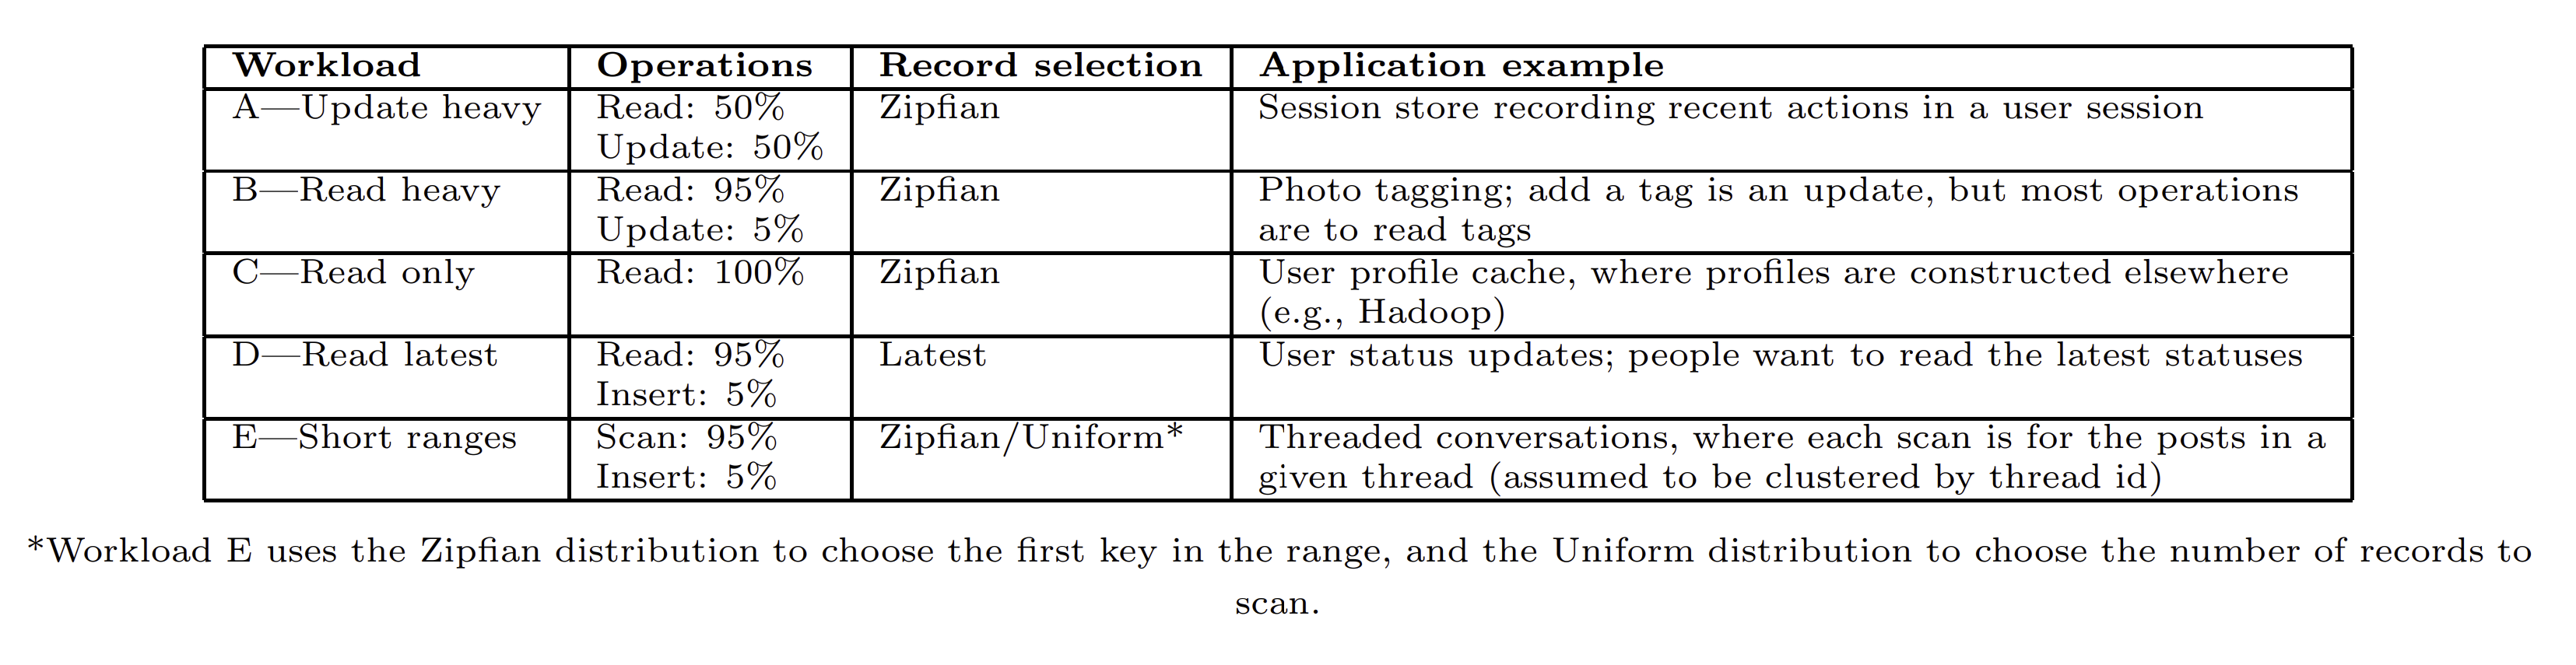
\includegraphics[width=0.8\textwidth]{images/ycsb.png}
  \caption{Definition of types of \ac{ycsb} workloads \parencite{ycsb}}
  \label{fig:ycsb}
\end{figure} 
\\\\
One early observation during the initial analysis was that the operation being benchmarked has a big influence on the measured \textit{time}. The idea of the thesis, however, is to find interpretable insights into which configurations influence the \textit{time} and how. Since the \textit{op} has a significant impact, and different configurations might benefit some operations more than others, the dataset is split into parts according to the feature \textit{op} and all the models are trained based on the respective parts. The box plot in figure \ref{fig:optime} represents the measured time of records for each operation type. The visible shift for each operation type, further supports the reason for splitting the data set, by highlighting the impact of single feature \textit{op} on the feature \textit{time}.

\begin{figure}[h]
  \centering
  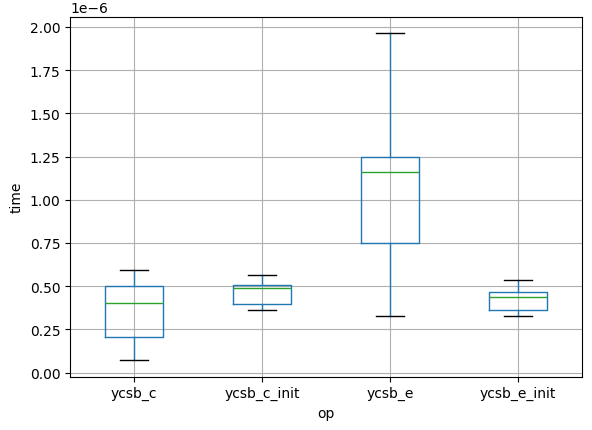
\includegraphics[width=0.5\textwidth]{images/boxplot_op.png}
  \caption{Box plot of time grouped by feature \textit{op}}
  \label{fig:optime}
\end{figure} 
\chapter{Approaches}\label{chapter:approaches}
In this chapter, the various approaches taken on getting insights using classical statistical, \ac{ML} and Data Mining techniques are explained. The actual outcomes of the \ac{ML} models and Data Mining algorithms are outlined in chapter \ref{chapter:findings}.

\section{Data exploration}
Before training \ac{ML} models it is important to understand what type of underlying data one is working with. The section \ref{chapter:preprocessing} on preprocessing explains the individual features and explains why the split of the data based on feature \textit{op} has been done. These findings originate from exploring the data in the first place, and understand which preprocessing steps are to be done to gain insights that are meaningful. One intuitive way to understand the relations between the features is by exploring the correlation between them. 

\subsection{Correlation}\label{correlationchapter}
A correlation, as the name suggests, describes the relationship between two features. In this thesis, the Pearson product-moment correlation coefficient is covered as defined by Salkind \parencite{salkind2011statistics}. This correlation coefficient measures the relationship between two values, giving a value in the range $[-1,1]$. Positive values for features X and Y indicate a relationship, where if the value of a feature X increases, the feature Y increases too. Negative values indicate the that the decrease of feature X results in an increase of feature Y. \\
The coefficient r between two features X and Y is calculated using the formula \ref{correlationformula}.

\begin{equation} \label{correlationformula}
r = \frac{n\sum_{i=1}^{n} (x_i - \bar{x})(y_i - \bar{y})}{\sqrt{n\sum_{i=1}^{n} (x_i - \bar{x})^2 \cdot n\sum_{i=1}^{n} (y_i - \bar{y})^2}}
\end{equation}
where:
\begin{align*}
r & \text{ is the Pearson correlation coefficient}, \\
n & \text{ is the number of data points}, \\
x_i \text{ and } y_i & \text{ are individual data points of X and Y}, \\
\bar{x} & \text{ is the mean of X}, \\
\bar{y} & \text{ is the mean of Y}.
\end{align*}
\\\\
This correlation can be calculated comparing all features, resulting in the correlation matrix as described by Papoulis et al. \parencite{papoulis2002probability}. It is symmetric along the diagonal, as the Person correlation is symmetric in nature as well. The figure \ref{fig:cormatrix} describes the correlation in the dataset collected in this thesis. Non-numeric features have been excluded for better viewability. It can be observed that the lower right section of the matrix displays high absolute values. This can be easily explained, since these features are output features, which are highly correlated between each other, including the target feature \textit{time}. 
\begin{figure}[h]
  \centering
  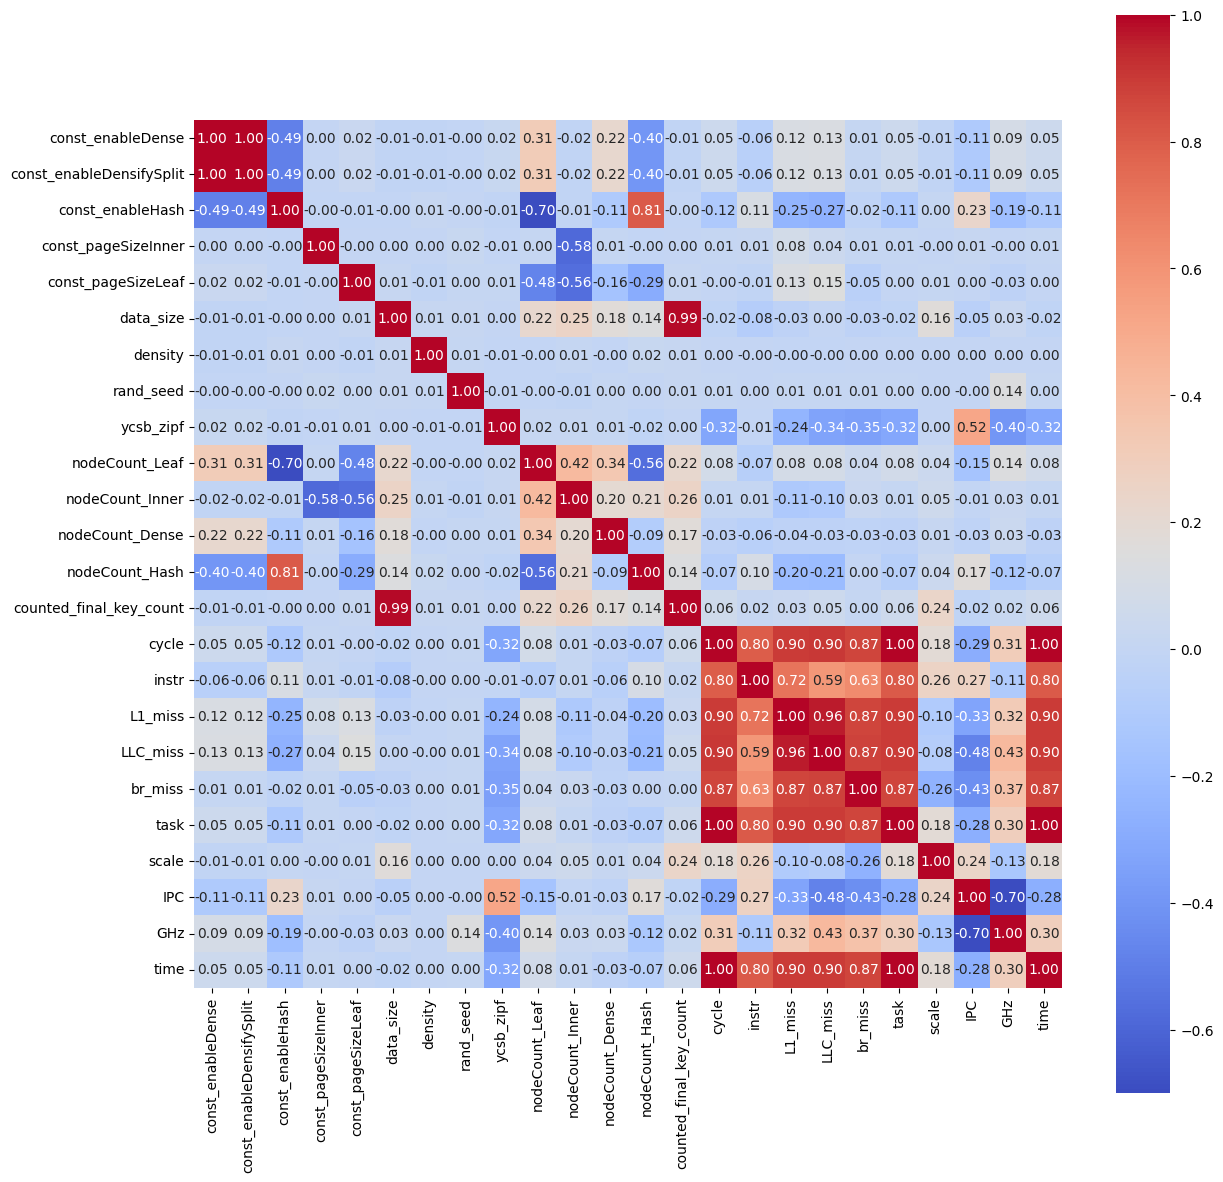
\includegraphics[width=0.8\textwidth]{images/correlation_matrix.png}
  \caption{Correlation matrix of the full dataset}
  \label{fig:cormatrix}
\end{figure} 
\\\\
Figure \ref{fig:cortime} represents the correlation coefficients between the feature \textit{time} and all other features. Some features are omitted from this figure, due to their constant values resulting in undefined behavior. The figure further highlights the high correlation between the output features and time, by displaying the output features in red and input features in blue. This highlights the importance of excluding these features as inputs to the \ac{ML} models. Including these features, would make it much easier for the \ac{ML} models to calculate the feature \textit{time} with high precision. However, such a scenario would be an inaccurate representation, since the output features are not available for new values and the goal of this thesis is to find correlation between input features and the feature \textit{time}.  
\\\\
Additionally, it can be observed that looking at the input features and their statistical correlation to feature \textit{time}, does not give promising insights, which is why \ac{ML} models are used to learn more complex relationships between the input and the feature \textit{time}. 
\begin{figure}[H]
  \centering
  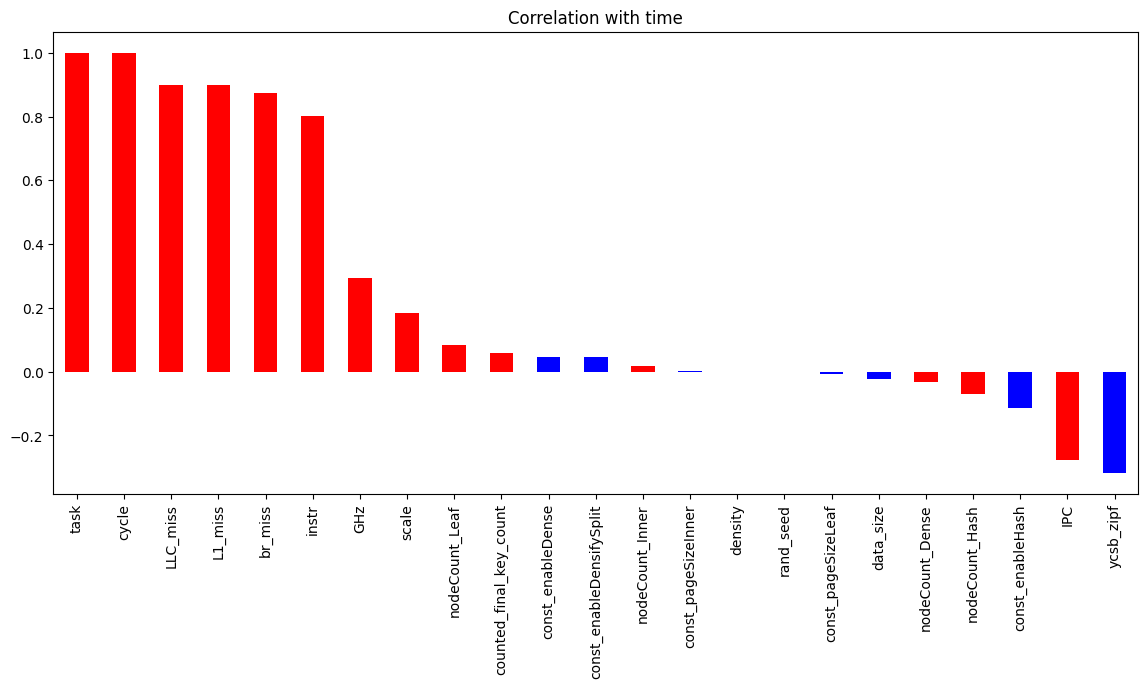
\includegraphics[width=0.8\textwidth]{images/correlation_with_time.png}
  \caption{Correlation of features with feature \textit{time}}
  \label{fig:cortime}
\end{figure}

\section{Classification models}
This section describes which classification models are used and what they do in a general sense. Before the individual \ac{ML} models are used, however, one needs to define, what is classified and what the metrics are used to distinguish good from bad models. In this thesis, the classification problem is defined as follows:
\\\\
Since the feature \textit{time} is a continuous value, it is not reasonable to classify each possible value as one class. Therefore, the values are split into 10 sections, based on the values. The class 1 indicates that the value is in the lowest 10\% of the data, meaning that it is among the fastest values. The class is stored as the feature \textit{percentile bracket}. For this, the following code is used to create the feature:

\begin{lstlisting}[language=Python]
df['percentile bracket'] = pd.qcut(df['time'], q=10, labels=False,
                                duplicates='drop') + 1
\end{lstlisting}
To make sure that the \ac{ML} model can be evaluated, a metric needs to be used on data, which the model has not been fed beforehand. Therefore, the data is split into a train- and a test set. This thesis uses an 80:20\% train/test split, which according to Joseph \parencite{joseph2022optimal} is a common ratio. In the paper \parencite{joseph2022optimal}, Joseph suggests using a ratio depending on the number of parameters, however, since this thesis aims to get insights into the data and not the best performing model, the simpler, static ratio split is applied.\\\\
Using the test set, a metric can calculate the usefulness of the model. The metric being used in this thesis is the accuracy score, as defined by \textit{scikit-learn} in \parencite{sklearnm19:online}. This score calculates the fraction of the correctly classified samples from the test set.
\\\\
Since the data has been split between the four values of feature \textit{op}, there are four models trained and therefore four metrics are compared per model type. 


\subsection{Decision Tree}
The Decision Tree classification, according to Zhou's definition in “Machine Learning” \parencite{zhou2021machine}, is a \ac{ML} model, which classifies data by creating a set of rules in a tree structure. The rules can be thought of if-then rules. At the leaf of the tree, the class of the value is defined. The Decision Tree can be built using a recursive algorithm, which continuously splits the set of data points in a node based on defined splitting rules until one of the termination conditions is met. In the book “Machine Learning” \parencite{zhou2021machine} Zhou defines the following three conditions on a node:
\begin{itemize}
  \item All data points are of the same class. 
  \item All data points have the same feature values, or there is no more feature to split. 
  \item There is no data point in the node.
\end{itemize}
The implementation that is used in this thesis \parencite{sklearnt33:online} allows further terminating conditions, such as the maximum depth of the tree, the maximum number of leaf nodes or a minimum number of data points required for a split of a node. 
\\\\
In the book “Machine Learning” \parencite{zhou2021machine}, Zhou further outlines that in order to determine the split, a higher \textit{purity} of the new child nodes is attempted to be achieved. The \textit{purity} is commonly measured by the \textit{information gain}, given in formula \ref{infogainformula}. Calculating the \textit{information gain} requires the \textit{entropy} of data, which is given in formula \ref{entropyformula}.  
\begin{equation} \label{entropyformula}
 \text{Ent}(D) = -\sum_{k=1}^{|y|} p_k \log_{2} p_k 
\end{equation}
where: 
\begin{align*}
\text{Ent}(D) & \text{ is the entropy of the data set}, \\
|y| & \text{ is the number of classes}, \\
p_k & \text{ is the proportion of the } k \text{th class}
\end{align*}
It is assumed that the classes are labelled $k=1,2,...,|y|$.
\begin{equation} \label{infogainformula}
\text{Gain}(D, a) = \text{Ent}(D) - \sum_{v \in \text{Values}(a)} \frac{|D_v|}{|D|} \text{Ent}(D_v)
\end{equation}
where:
\begin{align*}
\text{Ent}(D) & \text{ is the entropy of the dataset } D \\
\text{Values}(a) & \text{ is the feature} \\
|D_v| & \text{ is the number of instances for which feature } a \text{ has value } v \\
\text{Ent}(D_v) & \text{ is the entropy of the dataset } D_v
\end{align*}
The library \textit{scikit-learn} \parencite{sklearnt33:online} by default uses the splitting criterion \textit{Gini impurity} instead of \textit{entropy}. The \textit{Gini impurity}, according to Zhou \parencite{zhou2021machine} is defined in formula \ref{giniimpurityformula}.
\begin{equation} \label{giniimpurityformula}
\text{Gini}(D) = 1- \sum_{k=1}^{|y|} p_k^2
\end{equation}
where:
\begin{align*}
\text{Gini}(D) & \text{ is the Gini impurity of the dataset } D \\
|y| & \text{ is the number of classes} \\
p_k & \text{ is the proportion of the } k \text{th class}
\end{align*}
During experimentation of this thesis, practically, the results between using the criterion \textit{entropy} and \textit{Gini impurity} yielding minimal differences below a $0.5\%$ accuracy. Since no criterion yielded consistently better results, for the context of this thesis the criterion \textit{Gini impurity} is chosen. 
\\\\
Zhou \parencite{zhou2021machine} states that these formulae assume discrete values, which is why for continuous values a simple discretization technique is used, where the middle index of the sorted values is taken. This middle index is then used for splitting the feature values into two intervals, which can be taken as discrete values to calculate the splitting criterion.

\subsection{Random Forest}
The Random Forest classifier by \textit{scikit-learn} \parencite{sklearne64:online} takes the idea of a Decision Tree classifier and trains multiple Decision Trees with varied configurations. According to Zhou \parencite{zhou2021machine}, the variations vary the available features at each step. Additionally, the available data points are varied, with repeating data points across variations. 
\\\\
Zhou \parencite{zhou2021machine} further explains, that this method is part of the idea of Ensemble learning, where multiple models are trained and each value is then evaluated on all models and later the results are combined to give a final result. After training a given number of Decision Trees, the class is determined by giving one vote to each model. This method provides the benefit of better controlling over-fitting the models, since each time only a subset of data points from the training set is used. 

\subsection{Gradient Boosting}
According to Masui \parencite{AllYouNe72:online}, Gradient Boosting is an ensemble technique, which is built on the idea of training a "weak" decision tree and iteratively improving on it, by taking the loss function into account and using gradient descent. The loss function used in this thesis is the \textit{log\_loss}, which is the idea used in Logistic Regression \ref{LogisticRegression} and according to \textit{scikit-learn} \parencite{sklearne30:online} is a good idea for classification with probabilistic outputs. The figure \ref{fig:gradientboost} visualizes the flow of a Gradient Boosting model. The weights assigned to each "weak" decision tree is based on the loss function. The mechanism of how gradient descent is used in each iteration during training is out of the scope of this thesis.

\begin{figure}[H]
      \centering
      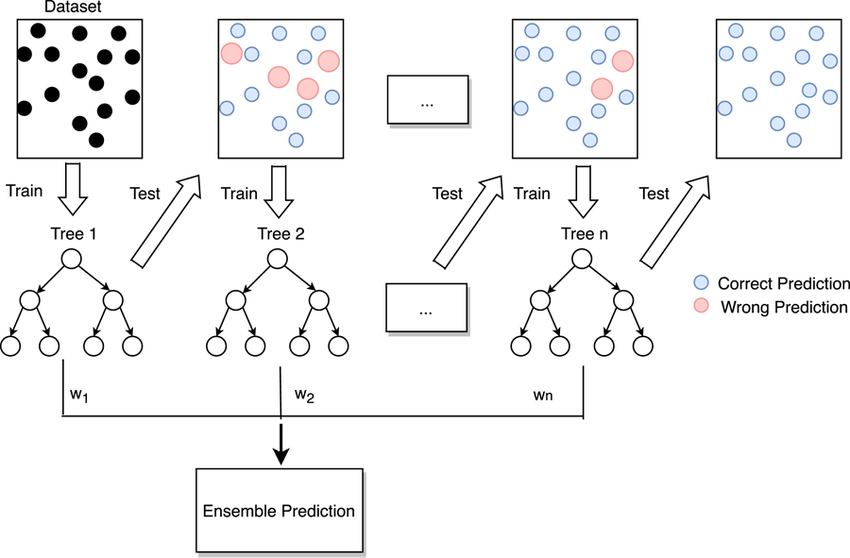
\includegraphics[width=0.5\textwidth]{images/gradientBoosting.png}
      \caption{Gradient Boosting flow diagram \parencite{gradientBoosting} }
      \label{fig:gradientboost}
  \end{figure}

\subsection{Neural network}
In the book \parencite{zhou2021machine} Zhou describes that there exist a number of types of neural networks, like Radial Basis Function networks, Adaptive Resonance Theory networks or Self-Organizing Map networks. However, the one described and used in this thesis is the Multilayer Perceptron (MLP) Classifier as defined by \textit{scikit-learn} \parencite{117Neura38:online}. According to Bishop \parencite{bishopML} the MLP is considered the most successful model, as it is of practical value for statistical pattern recognition. The MLP is also known as a feed-forward neural network. An example for an MLP is visualized in figure \ref{fig:mlp_sample}. The layer on the left is known as the input layer, where each node, also known as a neuron, represents one feature. The rightmost layer, the output layer, contains the output features, which in this example case is a scalar value, which in the case of MLP Classifiers would be the class of the value. The middle layer represents the hidden layer. There can be multiple hidden layers defined, each with a different amount of neurons. Additionally, each layer contains a \textit{bias}, typically referred to as the $0$th weight, $w_0$, in the layer. 
\begin{figure}[h]
      \centering
      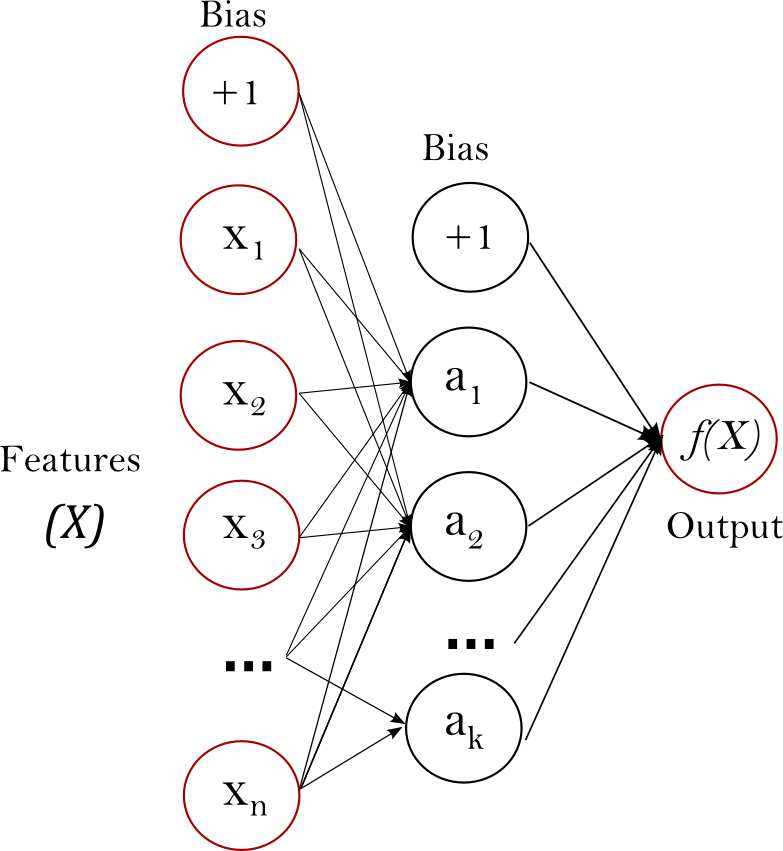
\includegraphics[width=0.5\textwidth]{images/mlp_example.png}
      \caption{MLP with one hidden layer \parencite{117Neura38:online} }
      \label{fig:mlp_sample}
  \end{figure}
As stated by Bishop \parencite{bishopML} and \textit{scikit-learn} \parencite{117Neura38:online}, each neuron, take the values from the previous layers and calculate a weighted sum $w_0 + w_1x_1 + w_2x_2 + ... + w_mx_m$, which consequently is put into a typically nonlinear activation function. Choosing the activation function can be done based on domain knowledge about the underlying data and its distribution.
\\\\
During experimentation of this thesis, the following activation functions yielded results with the highest accuracy. The \textit{ReLu} (Rectified Linear Unit) function $f(x)=max(0,x)$ and the \textit{Identity} function $f(x)=x$. In the end, \textit{ReLu} resulted in a slightly higher accuracy, therefore the results of this activation function are presented in the chapter on findings \ref{chapter:findings}.
\\\\
The neural network training process can be defined as follows:
\begin{enumerate}
    \item \textbf{Initialization}: The weights and biases are assigned random values.
    \item \textbf{Forward Pass}: At each layer the data from the previous layer is weighted summed, transformed and passed forward to the consequent layer.
    \item \textbf{Loss Calculation}: A loss function compares the calculated output for a validation set, which is not used in forward pass, with the actual output. 
    \item \textbf{Backpropagation}: The loss is then propagated backwards through the network by calculating gradients using mathematical techniques like the chain rule in calculus. 
    \item \textbf{Gradient Descent}: The gradients calculated in backpropagation are used to adapt the parameters in the loss-minimizing direction. Multiple Gradient Descent algorithms can be used, including \textit{Adam}, defined in \parencite{kingma2017adam}, and \textit{Stochastic Gradient Descent}. 
    \item \textbf{Iterations}: Steps 2 - 5 are iterated, gradually improving the network's performance. The training is terminated once the loss stops to decrease or starts to increase. Other terminating conditions can be set to the maximum number of iterations, time limit or by integrating other performance metrics. 
\end{enumerate}
This thesis does not delve into the detailed mathematical principles underlying backpropagation and gradient descent techniques. However, one characteristic of MLP Classifiers is that it is sensitive to feature scaling, which is why \textit{scikit-learn} \parencite{117Neura38:online} suggests using the \textit{StandardScalar}, as defined in \parencite{sklearnp90:online}, which transforms the data in such a way that each feature has a mean of zero and a standard deviation of one. This indeed improved the performance of some models trained in this thesis. In one case, this improvement increased the accuracy from around $4\%$ to more than $80\%$. The precise results are outlined and discussed in chapter \ref{chapter:findings}.

\subsection{Logistic regression} \label{LogisticRegression}
Despite what the name suggests, logistic regression actually is a classification model. The base case for logistic regression considers a binary classification, meaning that only two classes are considered, true and false. The logistic function, otherwise known as logistic sigmoid or sigmoid function, is used to identify the probability of an input belonging to a class. The logistic function is outlined in the formula \ref{logitfunc}. 
\begin{equation}\label{logitfunc}
    g(z) = \frac{1}{1 + e^{-z}}
\end{equation}
The figure \ref{fig:logitReg} visualizes the binary case of a logistic regression with one feature on the x-axis. The threshold value is set to 0.5 implying that results of the logistic function above 0.5 are classified as the class 1. 
\begin{figure}[h]
      \centering
      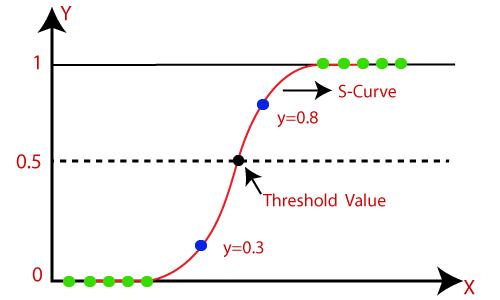
\includegraphics[width=0.5\textwidth]{images/logisticReg.png}
      \caption{Logistic regression example \parencite{Logistic19:online} }
      \label{fig:logitReg}
  \end{figure}
\\\\
The idea of binary classification case, can be extended to support multiple classes. The implementation used in this thesis extends the case by using \textit{multinomial logistic regression} with \textit{cross-validation}. This thesis does not go into the details of the multinomial logistic regression model, however the main idea can be summarized as follows.\\
To predict the class of a value the model takes a weighted sum of the input features for each possible class, puts the output into the softmax function, as defined in \ref{softmax}. These results are then put into the logistic function, which are then interpreted as the probability for each class. The most likely class is chosen to classify the value. \\ 

\begin{equation}\label{softmax}
    \text{softmax}(z_i) = \frac{e^{z_i}}{\sum_{j=1}^{K} e^{z_j}}
\end{equation}
\\
Following the suggestion of \parencite{CrossVal0:online}, to prevent overfitting and performing poorly on unseen data the cross-validation \textit{scikit-learn} implementation \parencite{sklearnl39:online} is used in this thesis. The concept is visualized in figure \ref{fig:crossval}. The training set is taken and split into $k$ disjoint subset. Afterward, each time a different subset is omitted from the training set and used as the testing set for that iteration. Following this, the results are averaged to create an evaluation result. This thesis set the parameter $k$ to 10, as it is, according to Zhou \parencite{zhou2021machine}, the most commonly used value.

\begin{figure}[h]
      \centering
      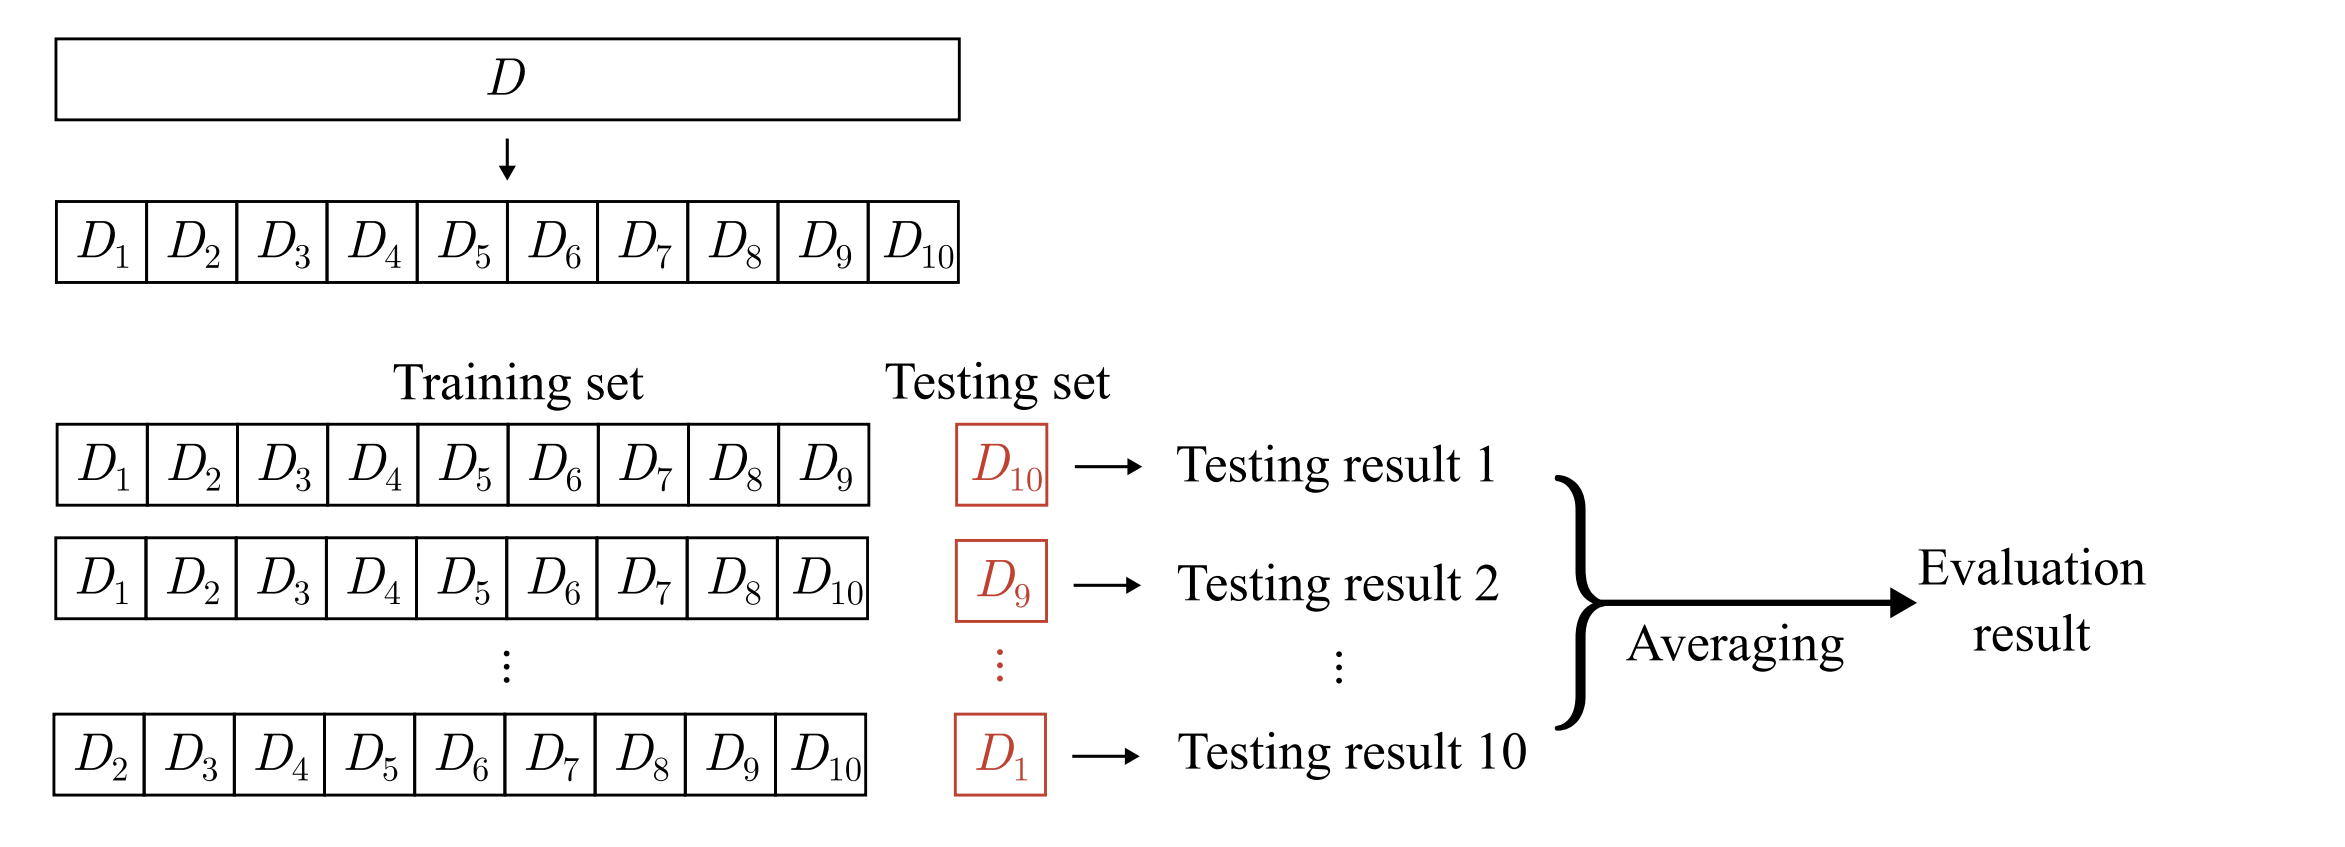
\includegraphics[width=0.5\textwidth]{images/crossvalidation.png}
      \caption{Cross validation example \parencite{zhou2021machine} }
      \label{fig:crossval}
  \end{figure}

\section{Regression models}
This section describes which \ac{ML} regression models have been used and gives an overview of how the individual models work. Since regression models are able to target a continuous feature, the target feature is the feature \textit{time}, without the need for more preprocessing.\\\\
To evaluate the performance of the models, the same procedure as with classification models with an 80/20 train/test split of data is employed. In contrast to the classification models, this thesis uses two metrics to evaluate the individual models.
\\\\
\textbf{RMSE} stands for Root Mean Squared Error, which, as the name suggests, is the root of the \textbf{MSE} metric. The MSE metric itself is the most commonly used metric, according to Zhou \parencite{zhou2021machine}, and it takes the mean of the squared errors, as defined in \ref{mseformula}. 
\begin{equation}\label{mseformula}
MSE = \frac{1}{n} \sum_{i=1}^{n} (y_i - \hat{y}_i)^2
\end{equation}
Despite the fact that RMSE is a metric in the same units as the target variable, this thesis uses the metric MSE. This is due to the already minuscule scale of the feature \textit{time}. 
\\\\
Additionally, since very small numbers are expected as errors, it is a good idea to make sure that the models actually perform better than the simplest model possible, which would be taking the average of the entire dataset. The \textbf{$R^2$}, as described by \textit{scikit-learn} in \parencite{sklearnm99:online}, also known as the coefficient of determination, typically yields results between 1, the perfect predictions, and 0, the average of the dataset. It can, however, also yield negative values, when the models perform more poorly than the average-case. The \textbf{$R^2$} is defined in formula \ref{rsquaredformula}
\begin{equation}\label{rsquaredformula}
R^2 = 1 - \frac{\sum_{i=1}^{n} (y_i - \hat{y}_i)^2}{\sum_{i=1}^{n} (y_i - \bar{y})^2}
\end{equation}
where:
\begin{align*}
R^2 & \text{ is the coefficient of determination} \\
n &  \text{ is the number of data points} \\
y_i & \text{ is the actual value of the } i^{th} \text{ record} \\
\hat{y}_i & \text{ is the predicted value of the } i^{th} \text{ record} \\
\bar{y} & \text{ is the mean of actual values of all records}
\end{align*}

\subsection{Linear regression}
According to Bishop \parencite{bishopML} the simplest linear model, and also the one used in this thesis, is the linear regression model. The model attempts to create a linear combination of input variable to create an output value. The model itself can be defined as in formula \ref{linregformula}. 
\begin{equation}\label{linregformula}
y = w_0 + w_1 x_1 + w_2 x_2 + \ldots + w_n x_n
\end{equation}
where:
\begin{align*}
y & \text{ is the target feature} \\
x_1, x_2, \ldots, x_n & \text{ are the features} \\
w_0, w_1, \ldots, w_n & \text{ are the weights representing the slopes of the regression line} 
\end{align*}
As Alto describes in \parencite{Understa37:online}, to estimate the weights of the Ordinary Least Squares (OLS) method is used, which minimizes the sum of squared differences. The details of this method include  differentiating the sum of squared differences with respect to each coefficient, setting the derivatives to zero, and solving the equation. 
\\\\
The implementation by \textit{scikit-learn} \parencite{11Linear83:online} assumes multiple characteristics. The main assumption is that there is a linear relationship between the input features and the target feature. Additionally, it is assumed, that each record is independent of the other records, which is the case in this thesis. 

\subsection{Random forest regression}
According to \textit{scikit-learn} \parencite{sklearne87:online}, decision trees can be used for classification, as well as regression. The key lies difference is that instead of taking the most occurring class in the leaf node, the mean of the target feature is taken. Similarly, to the decision tree for classification, the one for regression, can also face issues with over-fitting. The figure \ref{fig:regtree}, outlines this issue, by highlighting how defining the maximum depth can influence the outcome of the mode.
\begin{figure}[h]
      \centering
      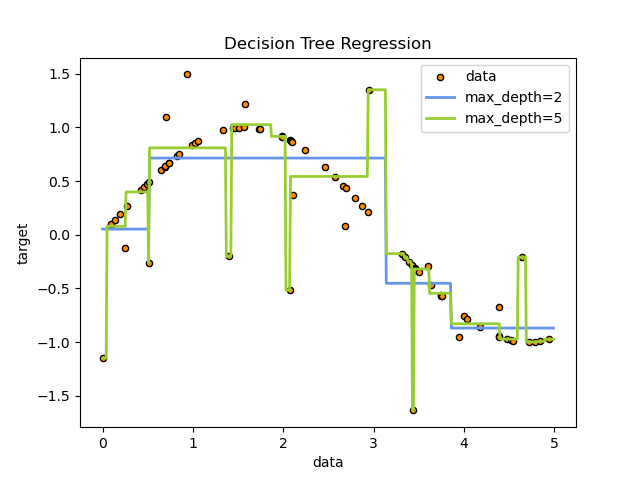
\includegraphics[width=0.5\textwidth]{images/regression_tree.png}
      \caption{Example for decision tree regression model \parencite{110Decis87:online} }
      \label{fig:regtree}
  \end{figure}
\\\\
To avoid the overfitting issue, the model RandomForestRegressor \parencite{sklearne87:online}, is trained which works on the same idea as described for the Random Forest Classification. 

\subsection{Gradient boosting regression}
Combining the idea behind Decision Tree Regression and Gradient Boosting Classification, the Gradient Boosting Regression model can be built. The major difference Gradient Boosting Classification is the fact that the underlying trees being built are regression in nature. 

\section{Pattern recognition}\label{patternreg}
As described in the blog \parencite{Frequent45:online}, pattern recognition is a set of algorithms that identify repetitive patterns in data. The pattern recognition algorithms described in this thesis differ from the classification and regression models in a major aspect. Instead of predicting target features on an unseen dataset, they bring insights into the underlying dataset, by highlighting patterns. This is very useful for the use-case of this thesis, due to the explainable nature.
\\\\
Before the algorithms described in this section are used, it is to be highlighted that a different dataset is used and additional preprocessing steps are executed on top of the ones described in chapter \ref{chapter:preprocessing}. Since the algorithms deal with discrete data with binary features, the dataset needs to be converted into such data. To ease these steps, the input parameters during benchmarking are limited to a defined set of possible values, instead of taking a random value in a given range. Additionally, less features are varied during the benchmarking, to avoid bloating the dimensionality of the data. To achieve the binary features, after dropping static features, \textbf{one-hot encoding} of all features is implemented. The exception to this is the feature \textit{time}, which before being one-hot encoded is split into three sections, similarly to the technique used for the classification models. The choice of three buckets instead of 10 used in classification stems from the limited variations of the input. The goal for these algorithms, in the context of this thesis, is to be able to identify which page size of leaf nodes performs faster for which B+ tree optimizations. 

\subsection{Apriori}
The Apriori algorithm, introduced by Agrawal et al. in \parencite{agrawal1994fast}, is used to identify frequent itemsets. These itemsets are later used in mining for association rules. The algorithm considers only one metric, the \textbf{support} which is defined as the fraction of the amount an itemset occurs in a dataset. After defining a support threshold, the algorithm returns the itemsets with a higher support. 
\\\\
The following example from the \textit{mlxtend} library \parencite{Apriorim11:online} outlines the algorithm. The transactions from figure \ref{fig:apriori1} yield for a minimum threshold of $60\%$ the frequent itemsets in figure \ref{fig:apriori2}.

\begin{figure}[H]
      \centering
      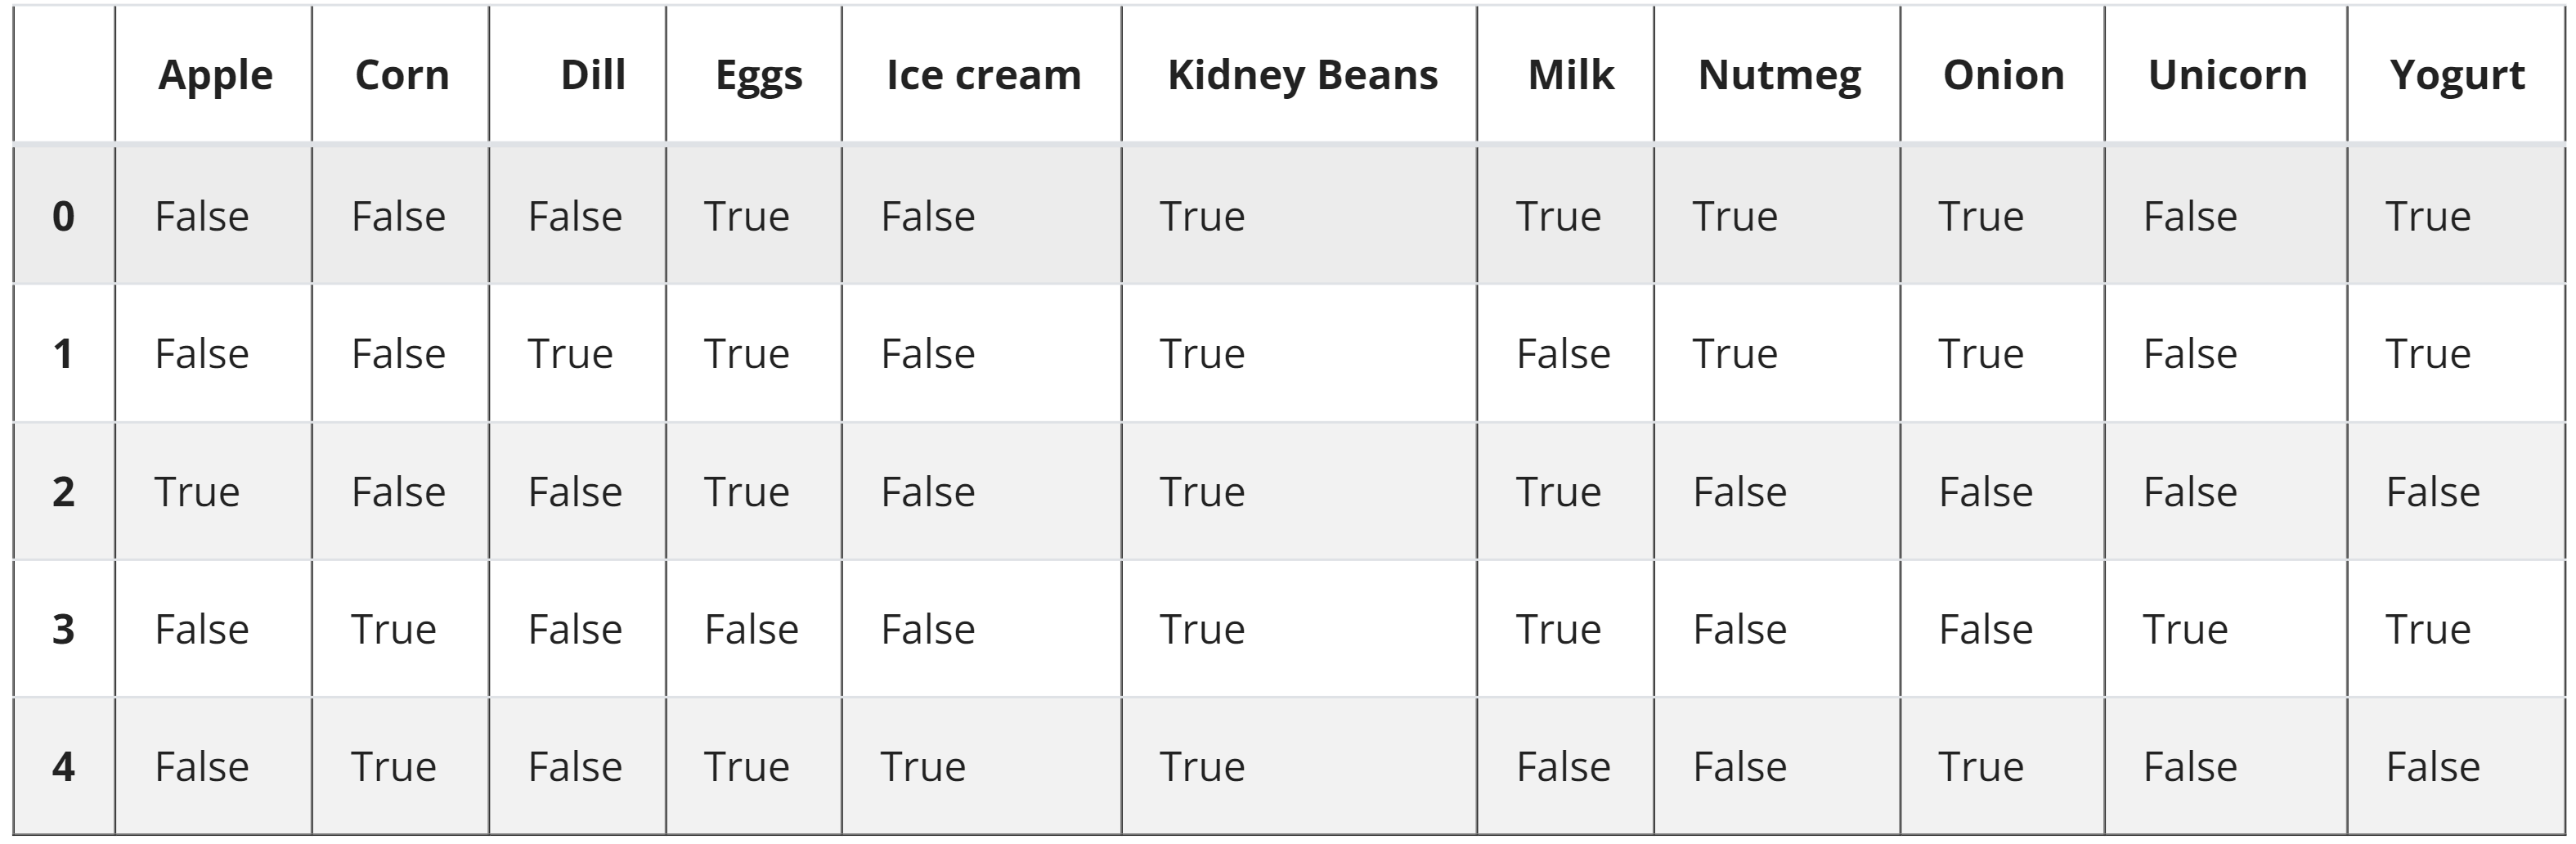
\includegraphics[width=0.5\textwidth]{images/apriori1.png}
      \caption{Apriori input example \parencite{Apriorim11:online} }
      \label{fig:apriori1}
  \end{figure}

\begin{figure}[H]
      \centering
      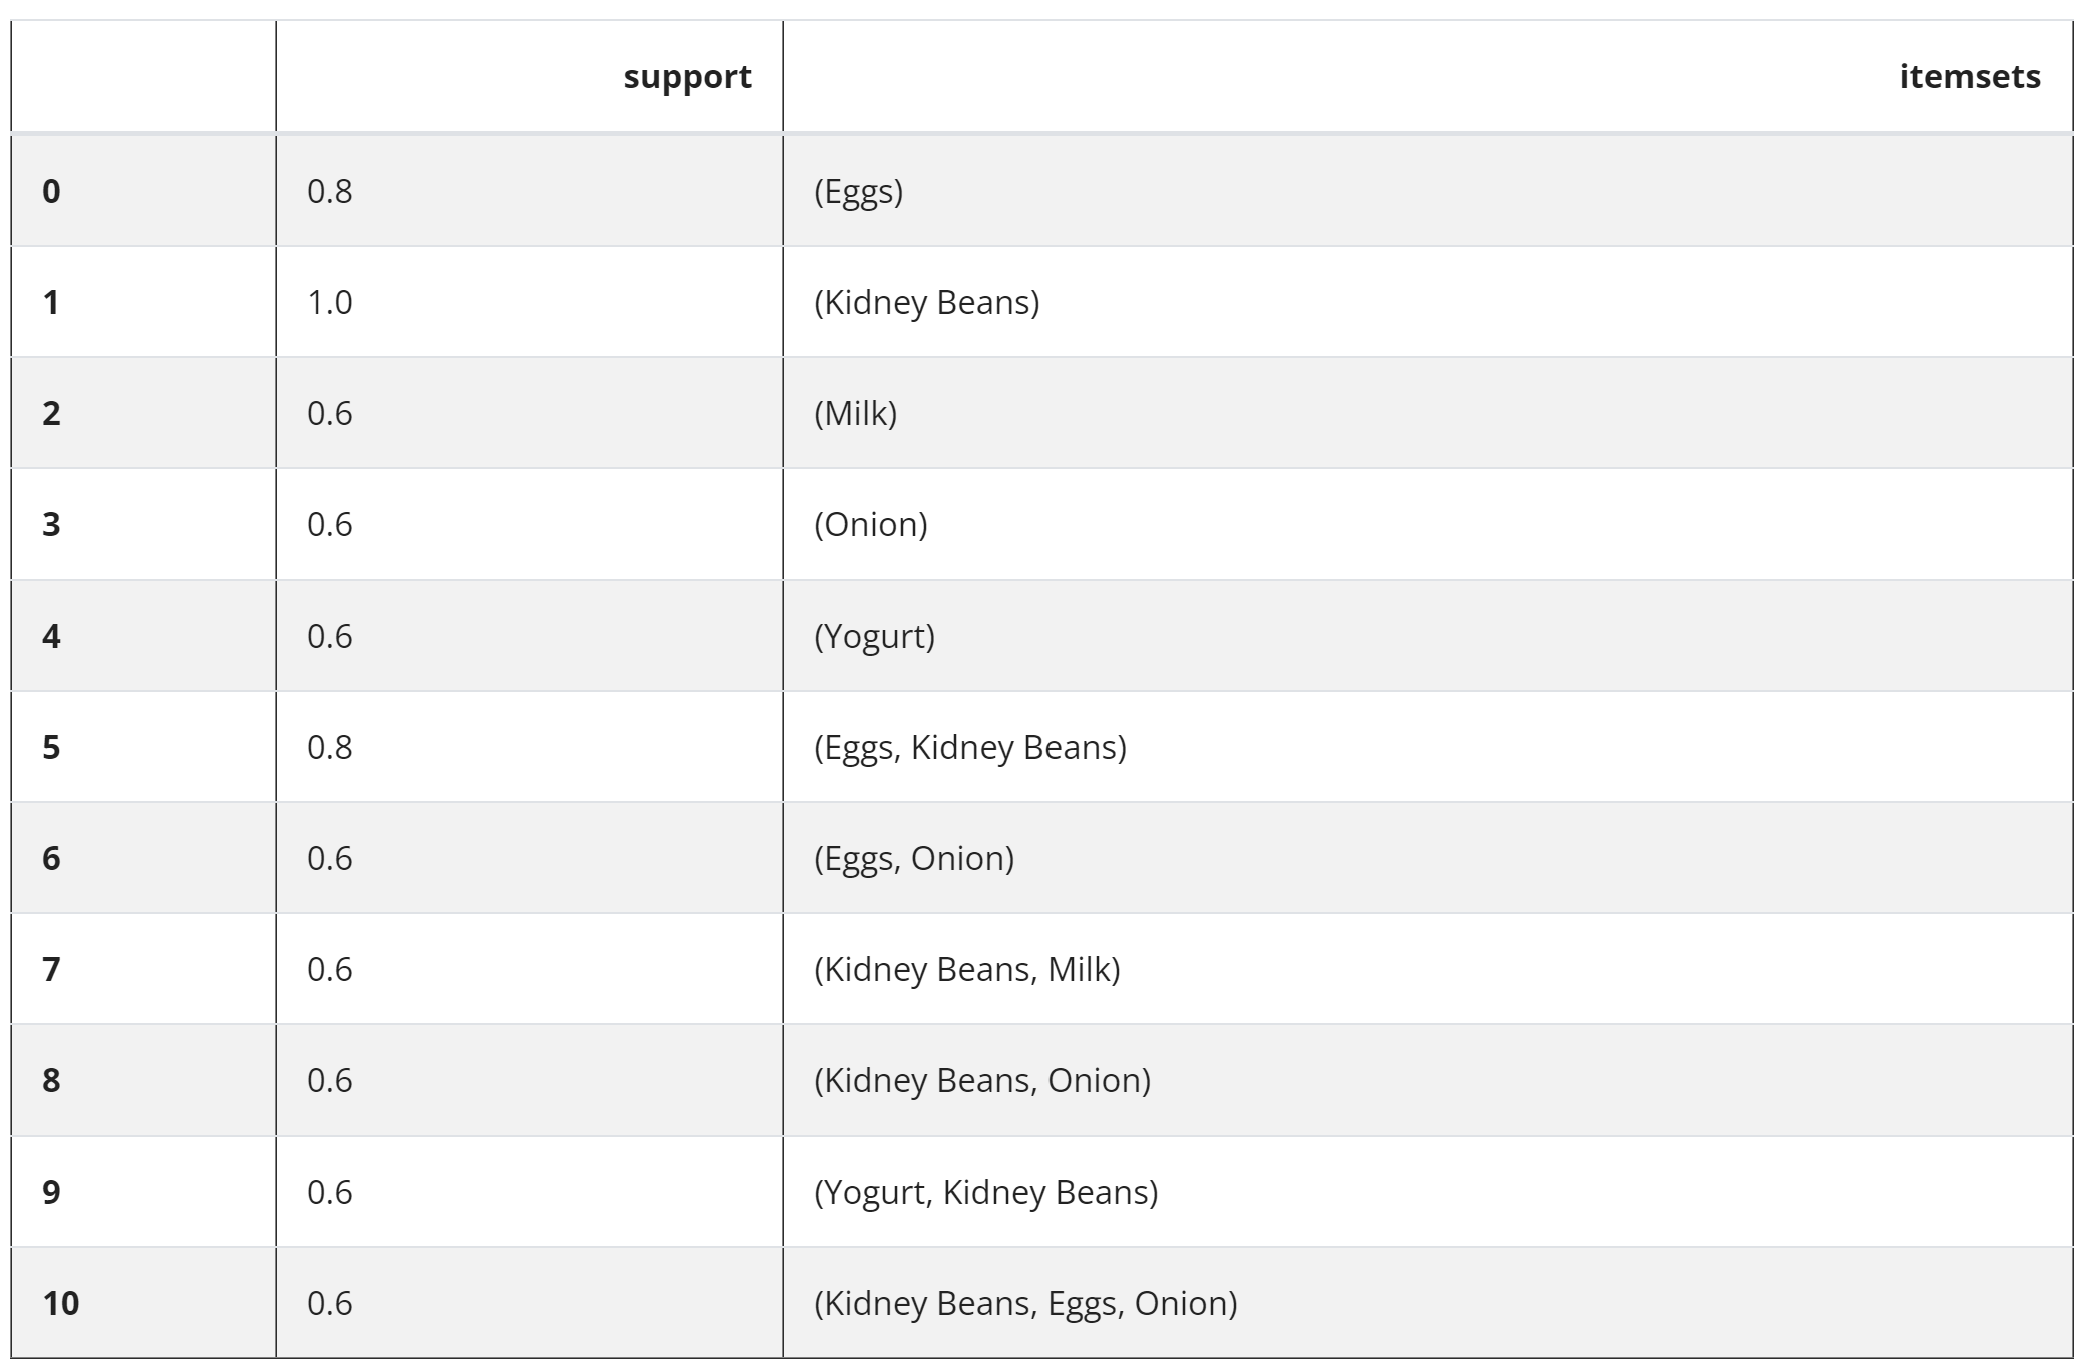
\includegraphics[width=0.5\textwidth]{images/apriori2.png}
      \caption{Apriori output example with $60\%$ support threshold \parencite{Apriorim11:online}}
      \label{fig:apriori2}
  \end{figure}

\subsection{Association rules}
The \textit{mlxtend} library describes association rules in its documentation \parencite{Associat99:online}, as rules in the form of $X \rightarrow Y$ with X and Y being disjoint itemsets. The rules imply the likely existence of $Y$ given that $X$ occurs.
\\\\
The implementation, from the \textit{mlxtend} library \parencite{Associat99:online} used in this thesis, takes the frequent itemsets created by the Apriori algorithm and generates rules based on those. It also allows limiting the output, by allowing to set a threshold for a metric. The implementation calculates various metrics for the rules, such as the ones used in this thesis support, confidence and lift.
\\\\
For $A \rightarrow C$, and A meaning antecedent itemset and C meaning consequent itemset the metrics used are defined by \textit{mlxtend} \parencite{Associat99:online} as follows: 
\begin{itemize}
    \item \textbf{Support:} Equal to the support of the union of the itemsets, described in Apriori algorithm.\\
    \begin{equation}
    \text{support}(A\rightarrow C) = \text{support}(A \cup C), \;\;\; \text{range: } [0, 1]
    \end{equation}
    
    \item \textbf{Confidence:} The conditional probability of finding the consequent item in a transaction given that the transaction contains the antecedent itemset.\\
    \begin{equation}
    \text{confidence}(A\rightarrow C) = \frac{\text{support}(A\rightarrow C)}{\text{support}(A)}, \;\;\; \text{range: } [0, 1]
    \end{equation}
    
    \item \textbf{Lift:} The ratio of the observed support to that expected if the items were statistically independent. It indicates the strength of a rule over random chance. Statistically independent itemsets would have the lift equal to 1. \\
    \begin{equation}
    \text{lift}(A\rightarrow C) = \frac{\text{confidence}(A\rightarrow C)}{\text{support}(C)}, \;\;\; \text{range: } [0, \infty]
    \end{equation}
\end{itemize}

\subsection{Optimal page size of leaf nodes}
To identify the most optimal size of leaf nodes, heatmaps can be generated, which visualize the features \textit{payload\_size} and \textit{data\_size} together with the best performing page size of leaf nodes. For this, two approaches are taken. One of the approaches is taking the dataset created for pattern recognition and training regression models on it. Then for each combination of the features \textit{payload\_size}, \textit{data\_size} and \textit{const\_pageSizeLeaf} the best performing page size is shown in the respective section. The other approach is skipping the regression model step and taking the empirical mean performance instead to identify the optimal page size. \\\\
The results of these approaches are outlined in chapter \ref{chapter:findings}. 
\chapter{XAI}\label{chapter:xai}

In his book "Interpretable Machine Learning" \parencite{molnar2022} Molnar describes the fundamentals of \ac{XAI}. This chapter is based on Molnar's findings. The idea behind \ac{XAI} is to be able to explain decisions made by an Artificial Intelligence, or \ac{ML} model. The ability to understand the underlying model's decisions can be crucial for real world applications of \ac{ML} models. One goal of \ac{XAI} is to increase the social acceptance of models by giving insights into why a model has made a certain decision. For example, in the application of self-driving cars, in the case of an accident, it is useful to understand why the car has made the decisions it has made and possibly even prove that the behavior prior to the accident was correct.
\\\\
For the case of this thesis, the goal of applying \ac{XAI} to the trained \ac{ML} models is to be able to understand which optimizations benefit from which configurations. 

\section{Characteristics of XAI techniques}
Since the topic of \ac{XAI} covers numerous algorithms, their characteristics can be broken down into whether a technique is \textbf{model-agnostic} or \textbf{model-specific} and whether it is a \textbf{local} or \textbf{global} explanation. The figure \ref{fig:xaioverview} provides an overview of these characteristics and how they relate to each other. 
\begin{figure}[h]
      \centering
      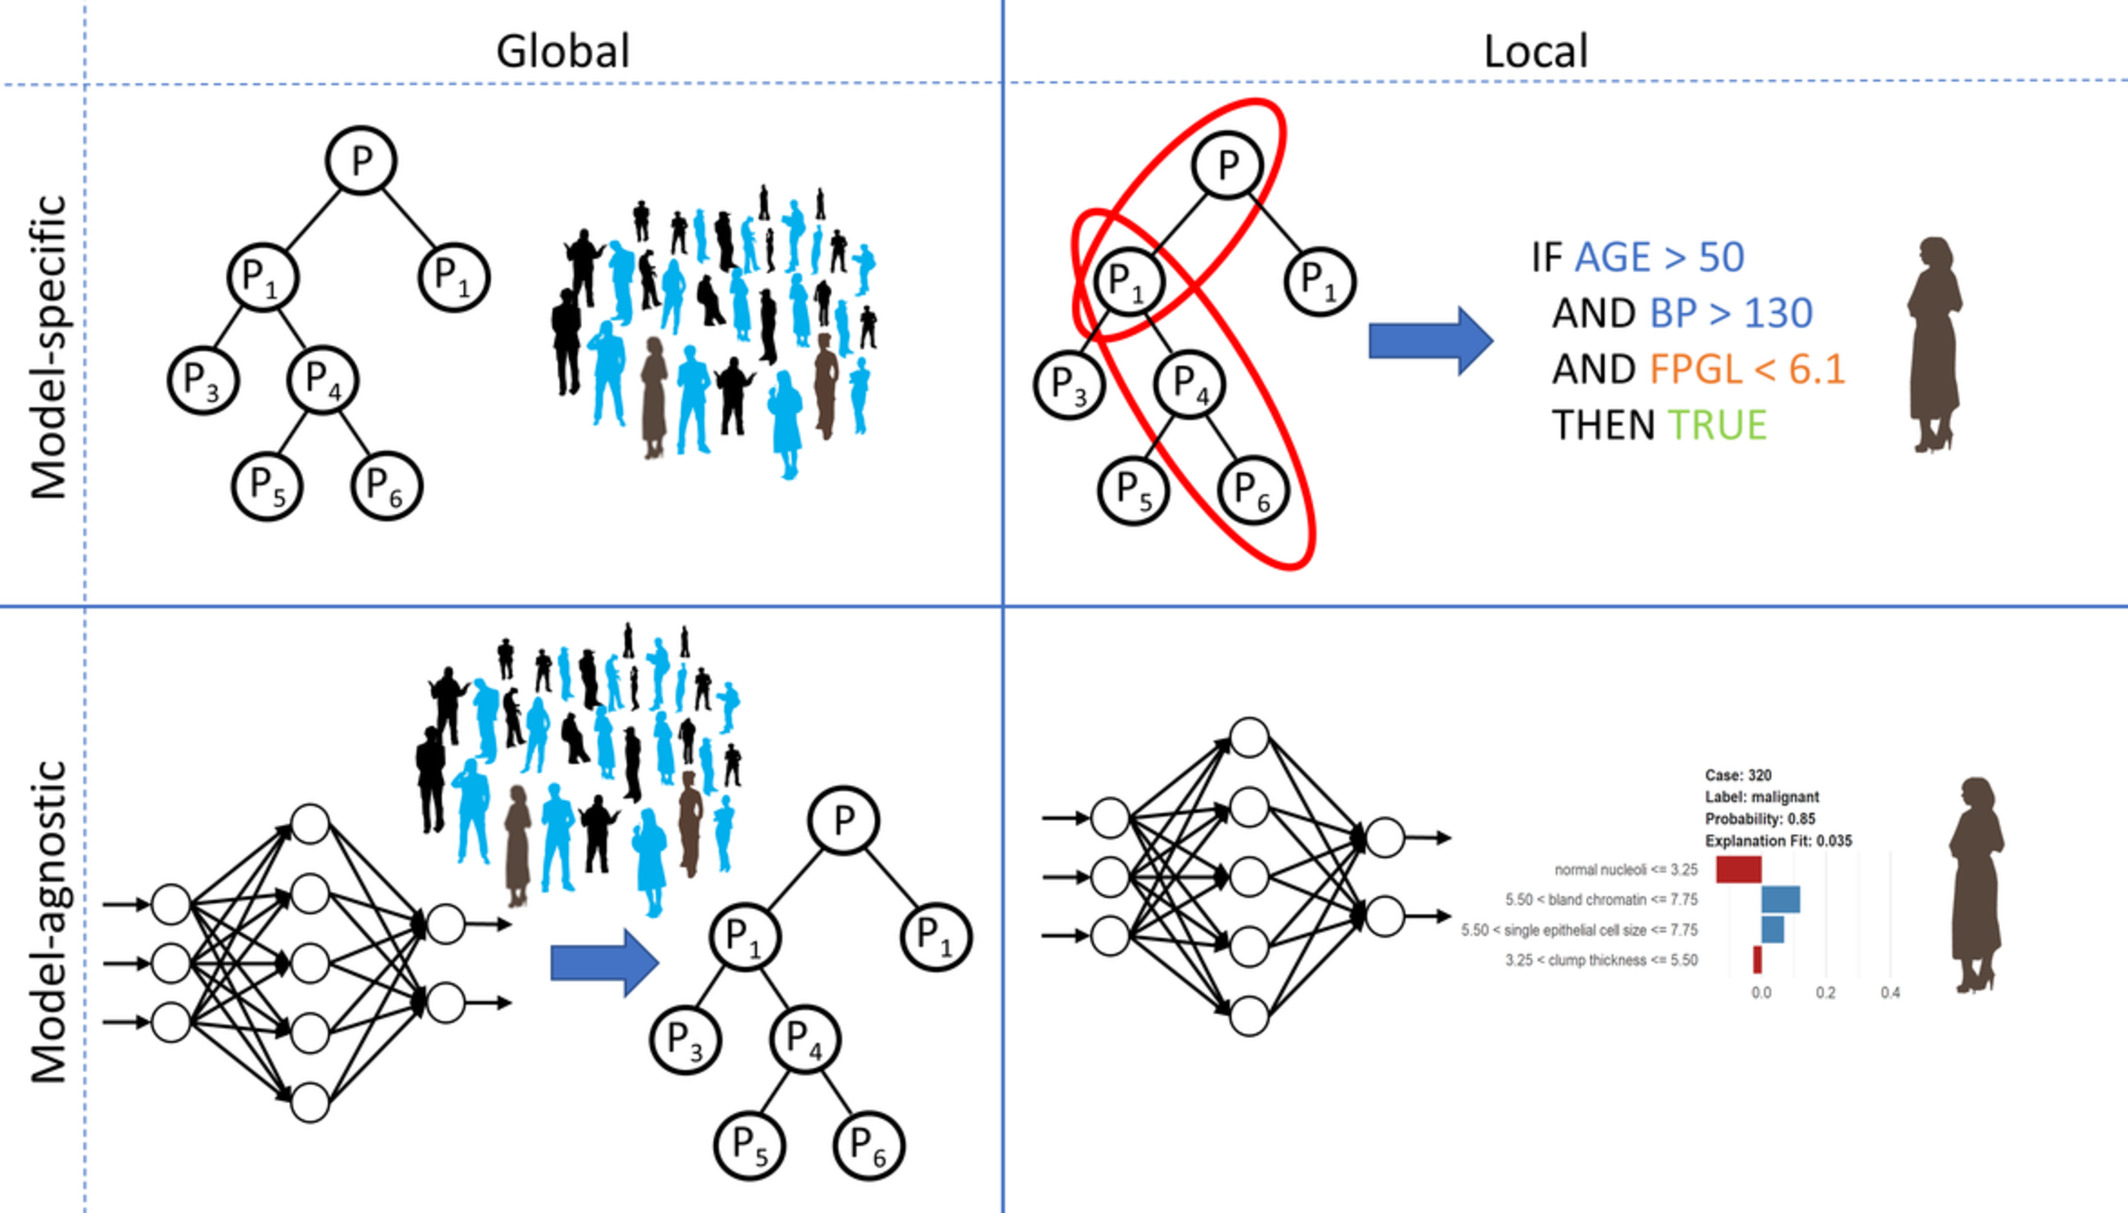
\includegraphics[width=0.8\textwidth]{images/XAI_overview.jpg}
      \caption{Overview of characteristics of XAI techniques \parencite{xaioverview}}
      \label{fig:xaioverview}
  \end{figure}
\\\
\textbf{Model-agnostic vs. model-specific}: Model-agnostic refers to techniques that can be applied to any \ac{ML} models. They consider the models as a black-box, meaning that they analyze the relationship between the inputs and the outputs and do not look deeper into the internal functionality of the models. Model-specific techniques are able to analyze the internal functionality of the models, but are limited to a specific type of models. These type of models can for example explain the weights of a linear model, or interpret the nodes in a neural network. 
\\\\
\textbf{Local vs. global}: Local \ac{XAI} techniques focus on interpreting the results of individual values, while global techniques interpret the model as a whole. Local techniques are not further discussed in this thesis, since interpreting individual runs of the benchmarking program does not provide a general picture about B+ tree configurations. They are more useful for real-world applications, where individual model decisions need to be explained. 
\\\\
\textbf{Model transparency}: Some machine learning models are considered transparent, or white-box, which refers to the interpretable nature of the model itself. Transparent models are considered to be easily humanly interpretable. A common case for this is a decision tree model, which is also used in figure \ref{fig:xaioverview} to represent explainable models. Not all transparent models are necessarily easily interpretable. For example, in the case of a decision tree model, if the tree has a big depth, the interpretations, can get incomprehensible. Linear models can be globally and locally explained, by analyzing the feature weights, however, there is the assumption that all features are statistically independent of each other.
\\\\
Out of the numerous algorithms that are part of \ac{XAI}, this thesis focuses on the algorithms that are suited for the use-case of this thesis. Model-specific interpretations are covered in the chapter \ref{chapter:findings}. It should be noted that the mathematical background of the individual algorithms is out of the scope of this thesis. Instead, this thesis aims to explain core ideas, the advantages, and disadvantages of the techniques.

\section{Permutation Feature Importance}
Permutation feature importance is a global model-agnostic method. The goal of this method is to identify, which features are important and which are less relevant. This is done by shuffling values of individual features and measuring the error of the model. One example of a permutation feature importance output, provided by the \textit{scikit-learn} implementation \parencite{42Permut82:online} used in this thesis, is presented in figure \ref{fig:permimp}. The plot highlights that the features \textit{sex}, \textit{pclass} and \textit{age} have the highest importance on an example model. Since various permutations are tested per feature, a box plot represents the output. 

\begin{figure}[H]
      \centering
      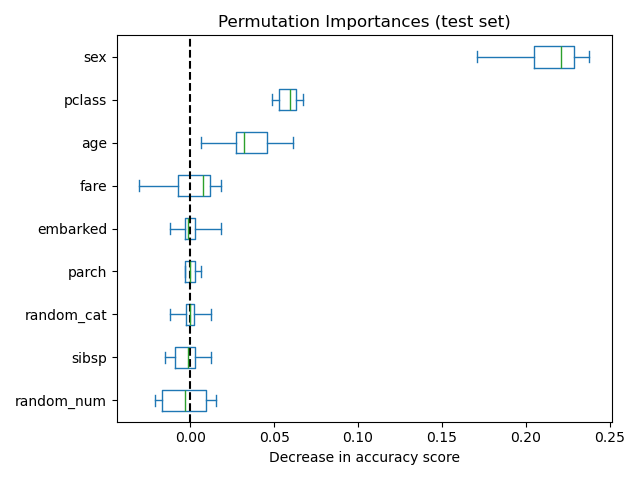
\includegraphics[width=0.5\textwidth]{images/feature_importance.png}
      \caption{Example output for permutation feature importance \parencite{42Permut82:online}}
      \label{fig:permimp}
  \end{figure}

\section{SHAP - SHapley Additive exPlanations}
SHAP is a technique that at its core is a local model-agnostic method. The idea behind this method is that a single record can be taken, and an individual feature is permuted to identify how the permutation impacts the result. The importance is measured in a so-called \textit{Shapley value}. KernelSHAP \parencite{shapKern53:online} is an algorithm used in this thesis, which trains a special weighted linear regression model to calculate the Shapley values of a record. For this thesis, however, local explanations are not relevant. \\
Nevertheless, KernelSHAP is used in this thesis, since applying the algorithm on multiple samples and plotting them in a \textbf{SHAP summary plot}, can give a broader, global picture about a model. An example for such a plot is given in figure \ref{fig:shapfeatimp}. This plot is beeswarm plot, where each dot represents a Shapley value of a record for each feature. The color of a dot indicates the value of a feature of a record from low to high. The density of the dots is visualized by stacking dots along the y-axis. The features are sorted from the highest mean of absolute Shapley values to the lowest.
\\\\
One can compare the SHAP summary plot to the permutation feature importance. They both intend to outline the feature importance, however the difference lies in the underlying structure of the algorithms. Permutation feature importance calculates the error by permuting features for all values, while SHAP feature importance takes the average impacts of features for individual values.

\begin{figure}[H]
      \centering
      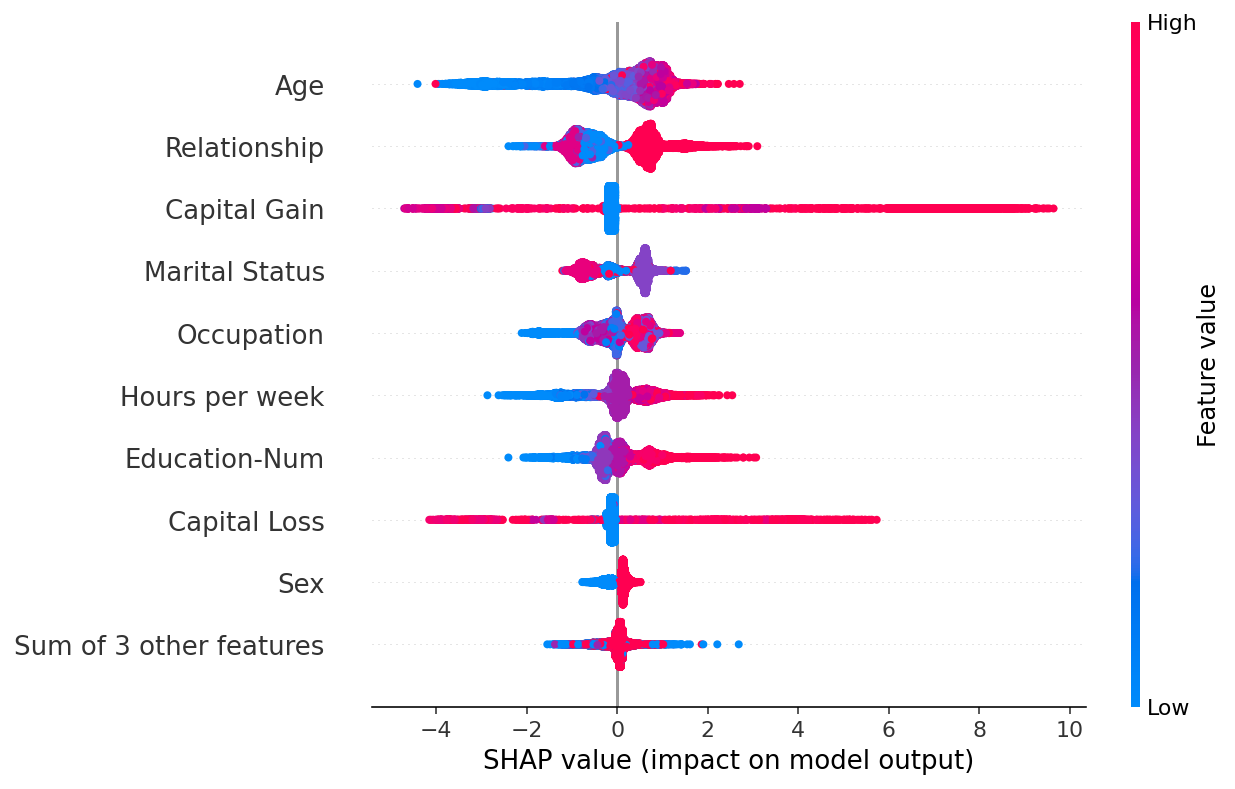
\includegraphics[width=0.7\textwidth]{images/SHAP_example.png}
      \caption{Example output for SHAP feature importance \parencite{barplot—98:online}}
      \label{fig:shapfeatimp}
  \end{figure}

\chapter{Findings}\label{chapter:findings}
This chapter collects the results of the individual models, the \ac{XAI} algorithms, and pattern recognition algorithms. The results are then analyzed and interpreted.

\section{Classification Models}
After doing all the preprocessing steps mentioned in chapter \ref{chapter:preprocessing}, the classification models have yielded the results visualized in figure \ref{fig:classification_performance}. The results indicate that ensemble methods, random forest and gradient boosting, seem to perform better than a classic random tree. The neural network classifier, however, performs best for all operations, with the exception of \textit{ycsb\_e\_init}, where gradient boosting performs better by a minimal difference of less than one percent. A surprising observation is the difference of performance between the initialization operations. This is attempted to be explained by the XAI techniques.
\begin{figure}[h]
      \centering
      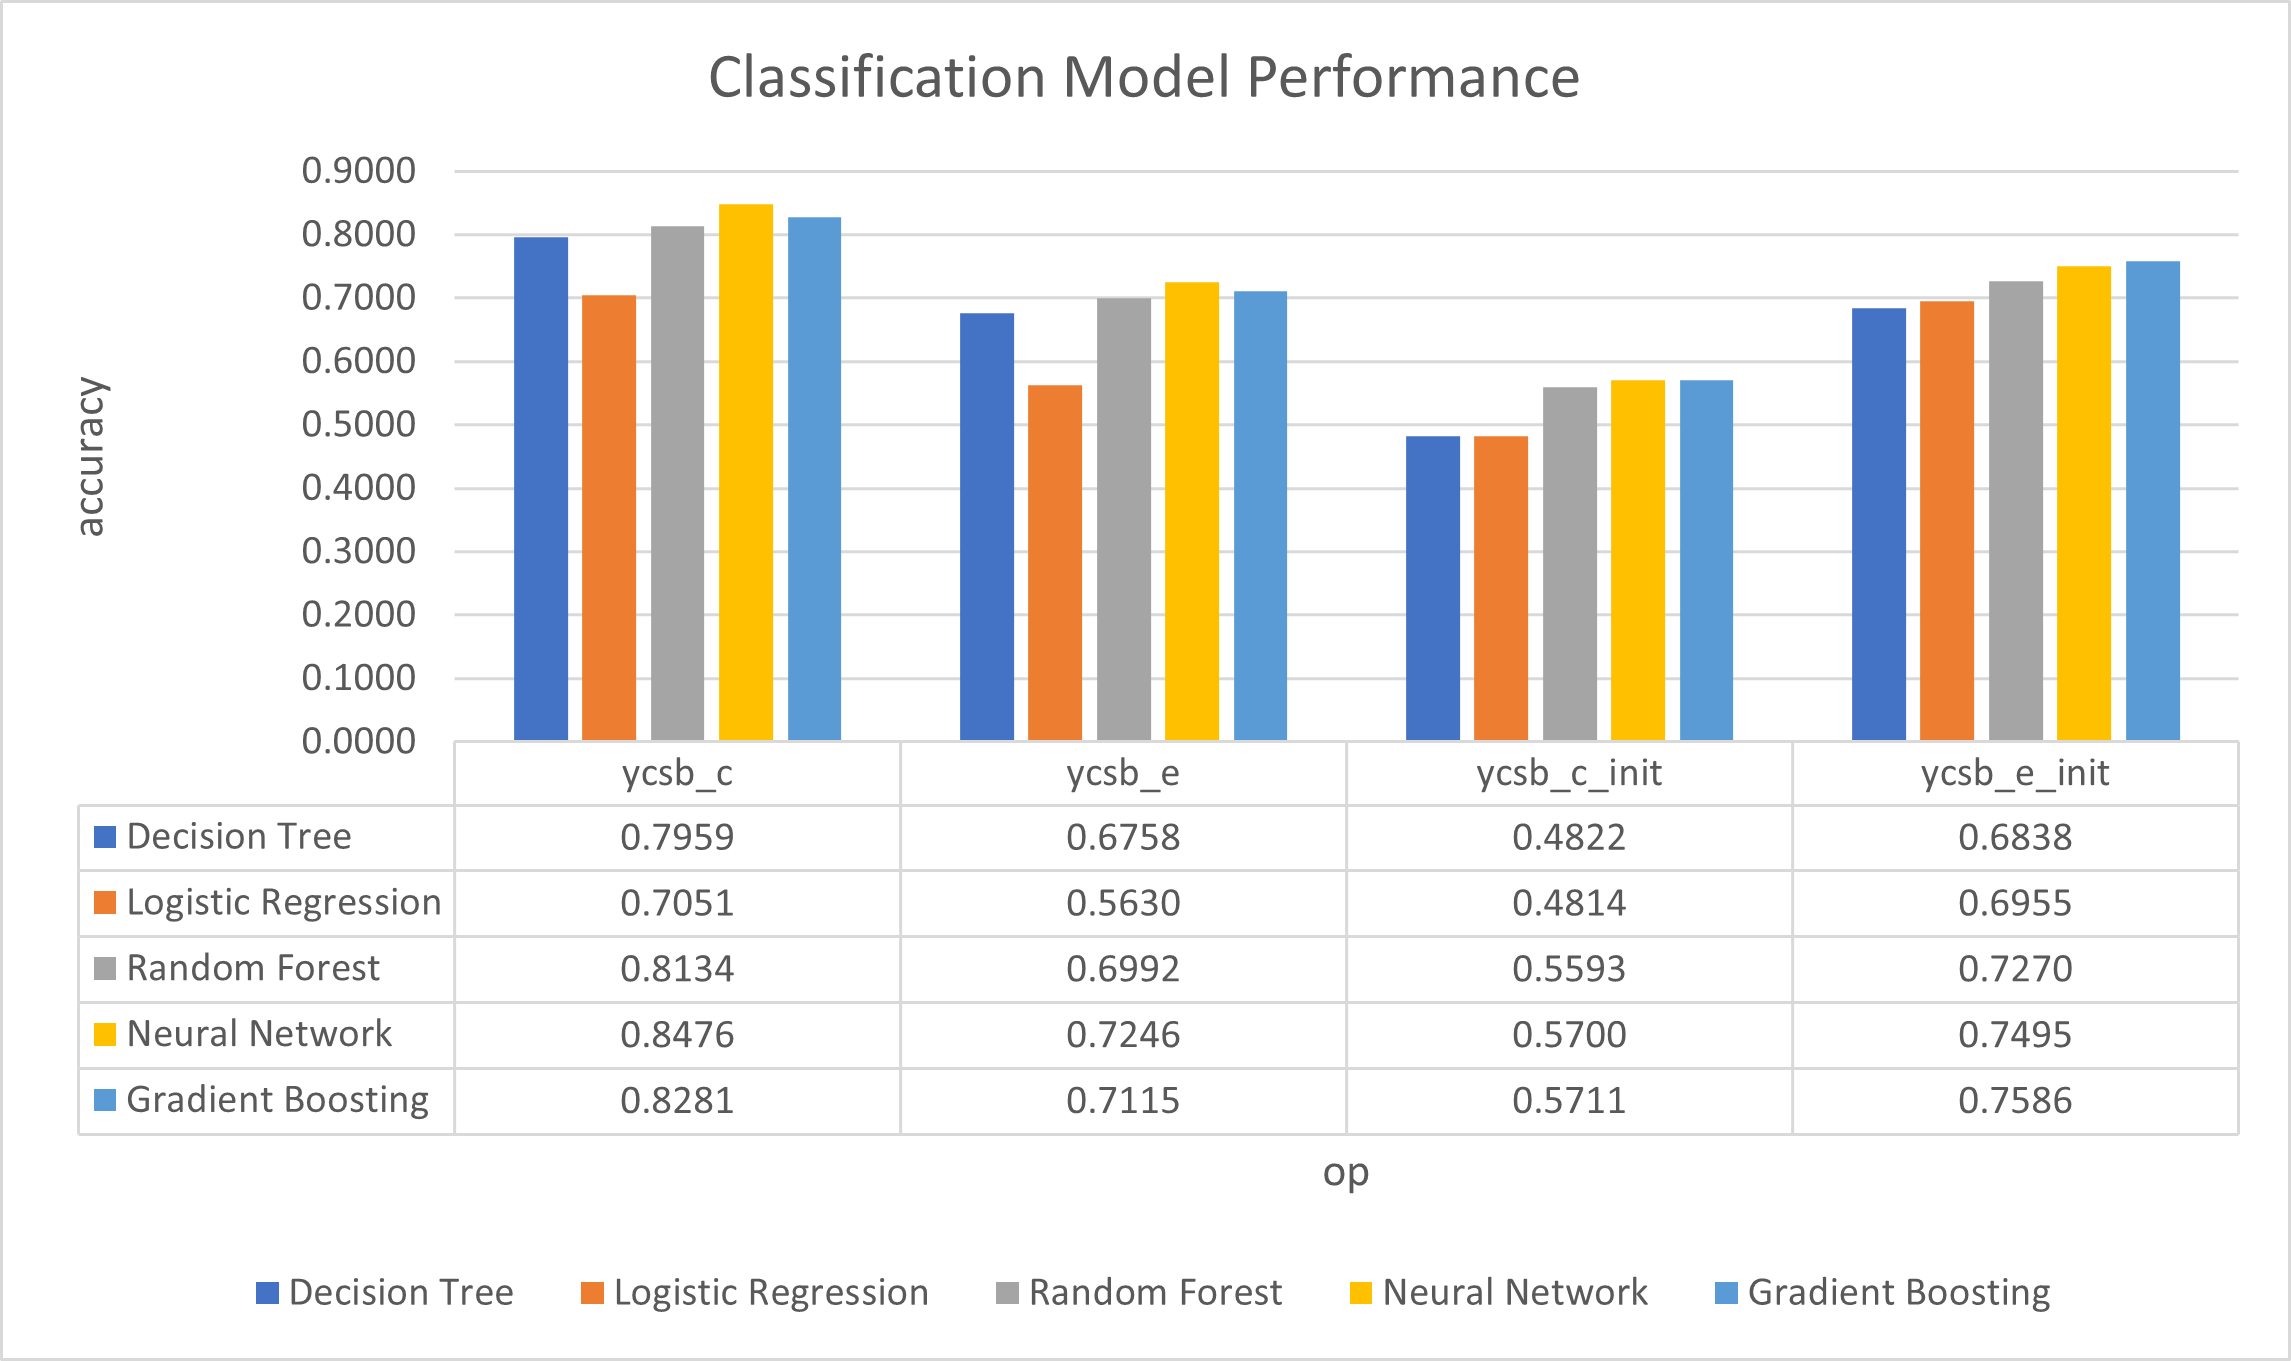
\includegraphics[width=0.85\textwidth]{images/classification_performance.png}
      \caption{Graph and data for performance of classification models}
      \label{fig:classification_performance}
  \end{figure}
\\\\
The generally best performing model in all cases, the neural network, has been further analyzed for each operation. This is done using \ac{XAI} techniques mentioned in chapter \ref{chapter:xai}. It should be noted that similar figures have been created for the gradient boosting models during experimentation, and therefore only the insights from the best performing models are shown and discussed. \\

\subsection{Permutation Feature Importance}
Figure \ref{fig:nnfeatimp} depicts four box-plots generated by applying the permutation feature importance algorithm on the neural networks created for the four operation types.
\begin{figure}[h]
      \centering
      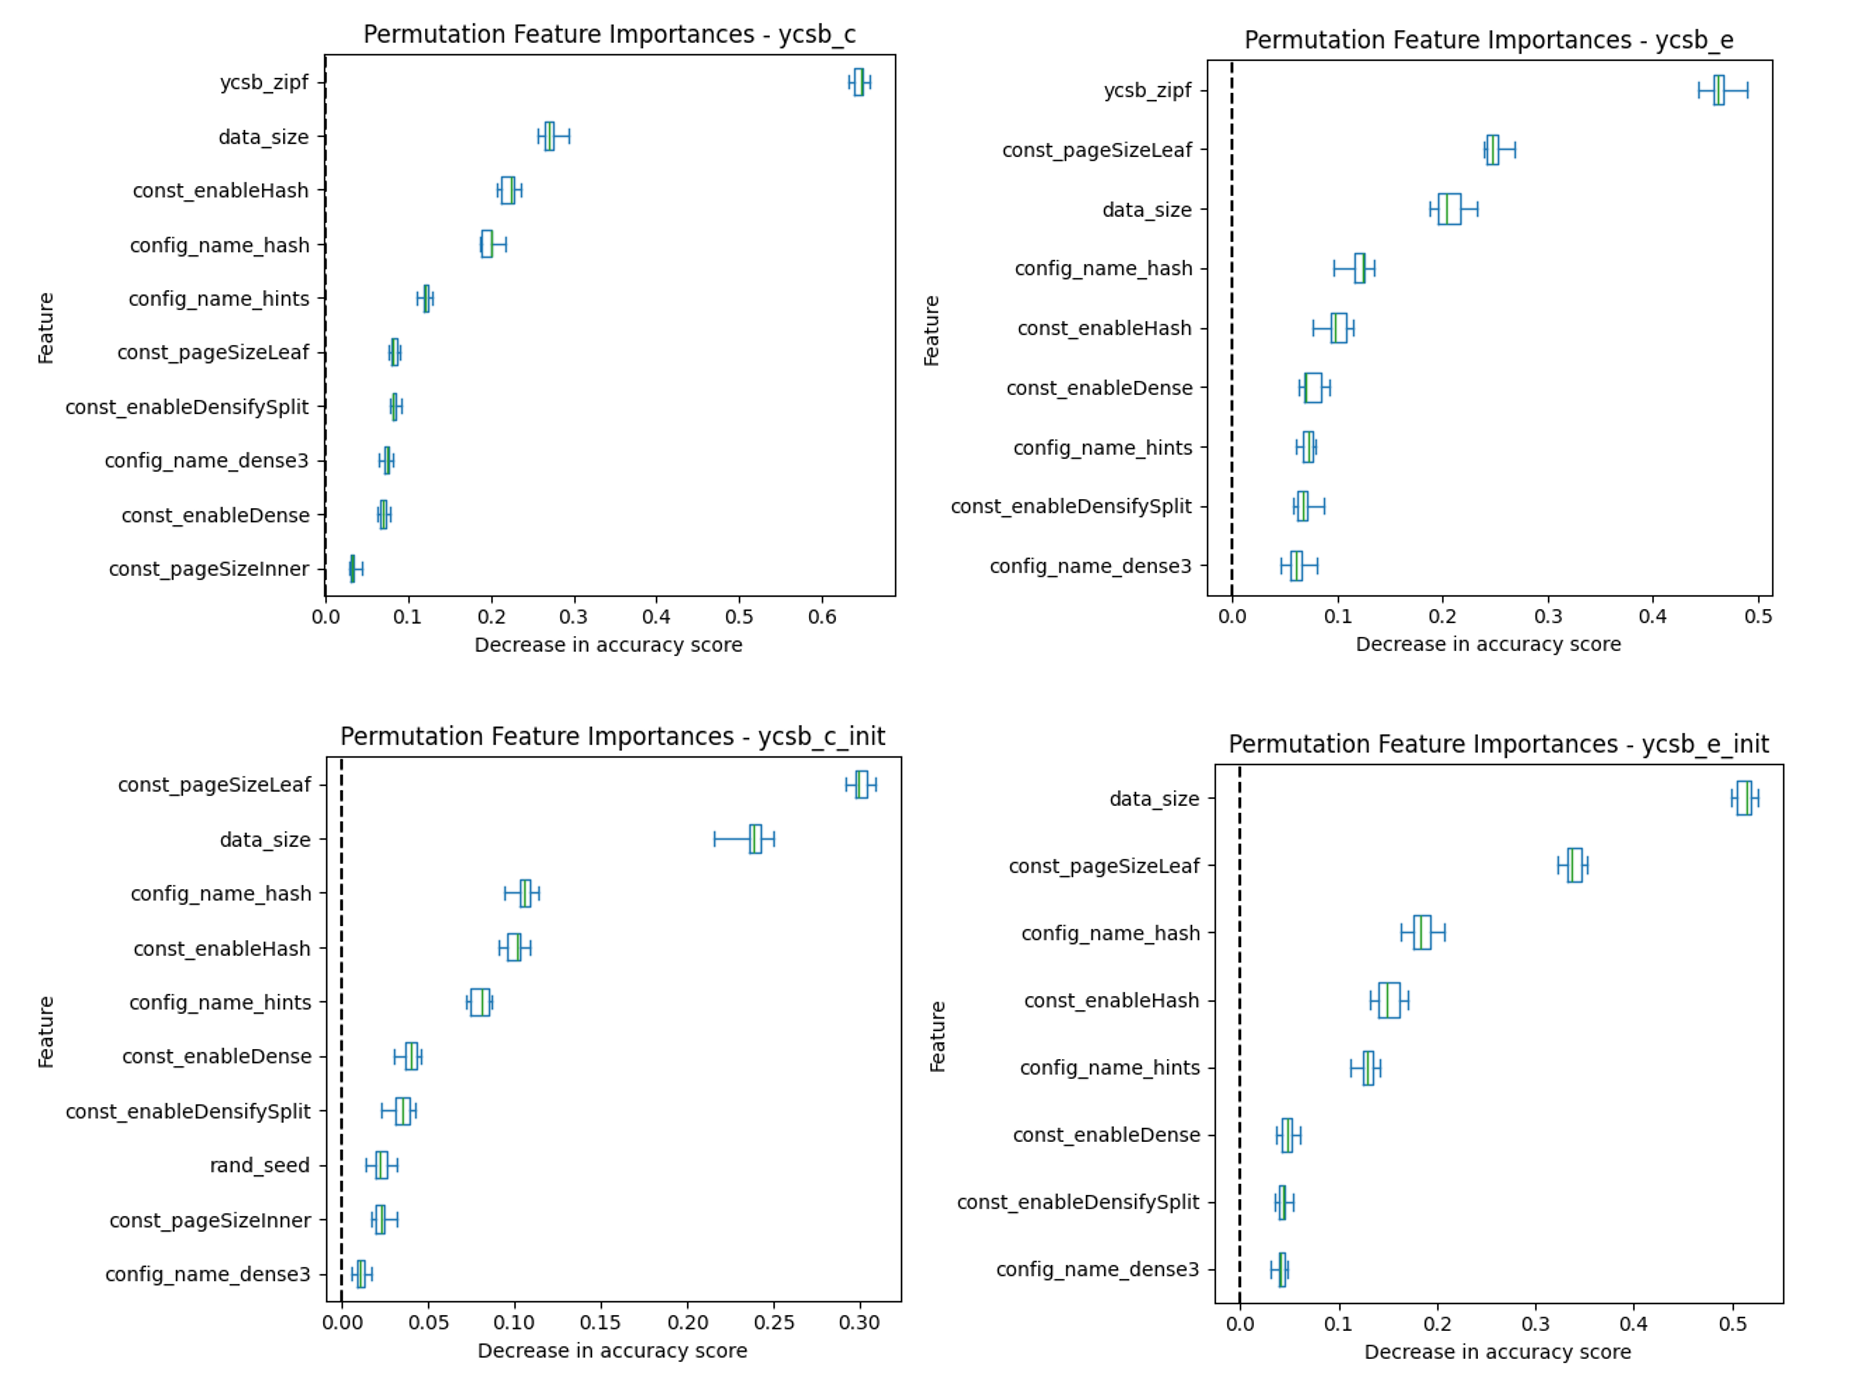
\includegraphics[width=0.9\textwidth]{images/nn_fi.png}
      \caption{Neural network permutation feature importances}
      \label{fig:nnfeatimp}
  \end{figure}
\\\\
The most notable result is that the feature \textit{ycsb\_zipf}, which describes how skewed the distribution of accessed keys is, is the most important feature for the benchmarking operations. For the initialization, the feature has no importance, which can be explained by the fact that the initialization operations do not consider the skewness during the run. 
\\\\
Furthermore, it can be seen that for operations that perform insertions (\textit{ycsb\_e}, \textit{ycsb\_e\_init}, \textit{ycsb\_c\_init}) the feature \textit{const\_pageSizeLeaf} has a higher importance. The \textit{data\_size} is important for all operations, which can be explained by the fact that the B+ tree grows with more data and therefore the operations require more time to read and insert.
\\\\
Since the features \textit{const\_enableHash} and \textit{config\_name\_hash} are highly correlated, it is understandable why the features are assigned similar importance. The slight differences could be explained by the random permutations that occur during the creation of the plot. 
\\\\
One should not assume that a higher importance of a configuration name implies a better performance. For example, the higher importance of \textit{config\_name\_hash} than \textit{config\_name\_dense3} only implies that when the models classify more based on the \textit{config\_name\_hash} than \textit{config\_name\_dense3}. To understand which configurations lead to which classification, one could use local \ac{XAI} techniques or use pattern recognition to identify these patterns. This, however, is beyond the objectives of this paper. 
\\\\
An unexplained phenomenon is the differences between the initialization operations. The feature \textit{data\_size} seems to be much more important for the operation \textit{ycsb\_e\_init}, compared to \textit{ycsb\_c\_init}. This could potentially explain the difference in the performance for the models. It could lie in the fact that for these two operations, the feature \textit{scale} is calculated differently, which impacts the target feature \textit{time} and consequently the models too. The feature \textit{scale} is set for the \textit{ycsb\_c\_init} to the number of keys, while for \textit{ycsb\_e\_init} $2.5\%$ is subtracted from that number. The subtraction is due to the fact that operation \textit{ycsb\_e} is expected to insert that amount of keys in its benchmark. However, validating this theory falls beyond the purview of this thesis.

\subsection{SHAP Summary Plot}
Figure \ref{fig:shap_sum} depicts four SHAP summary plots generated by applying the KernelSHAP algorithm and plotting the results of the neural networks created for the four operation types.
\begin{figure}[h]
      \centering
      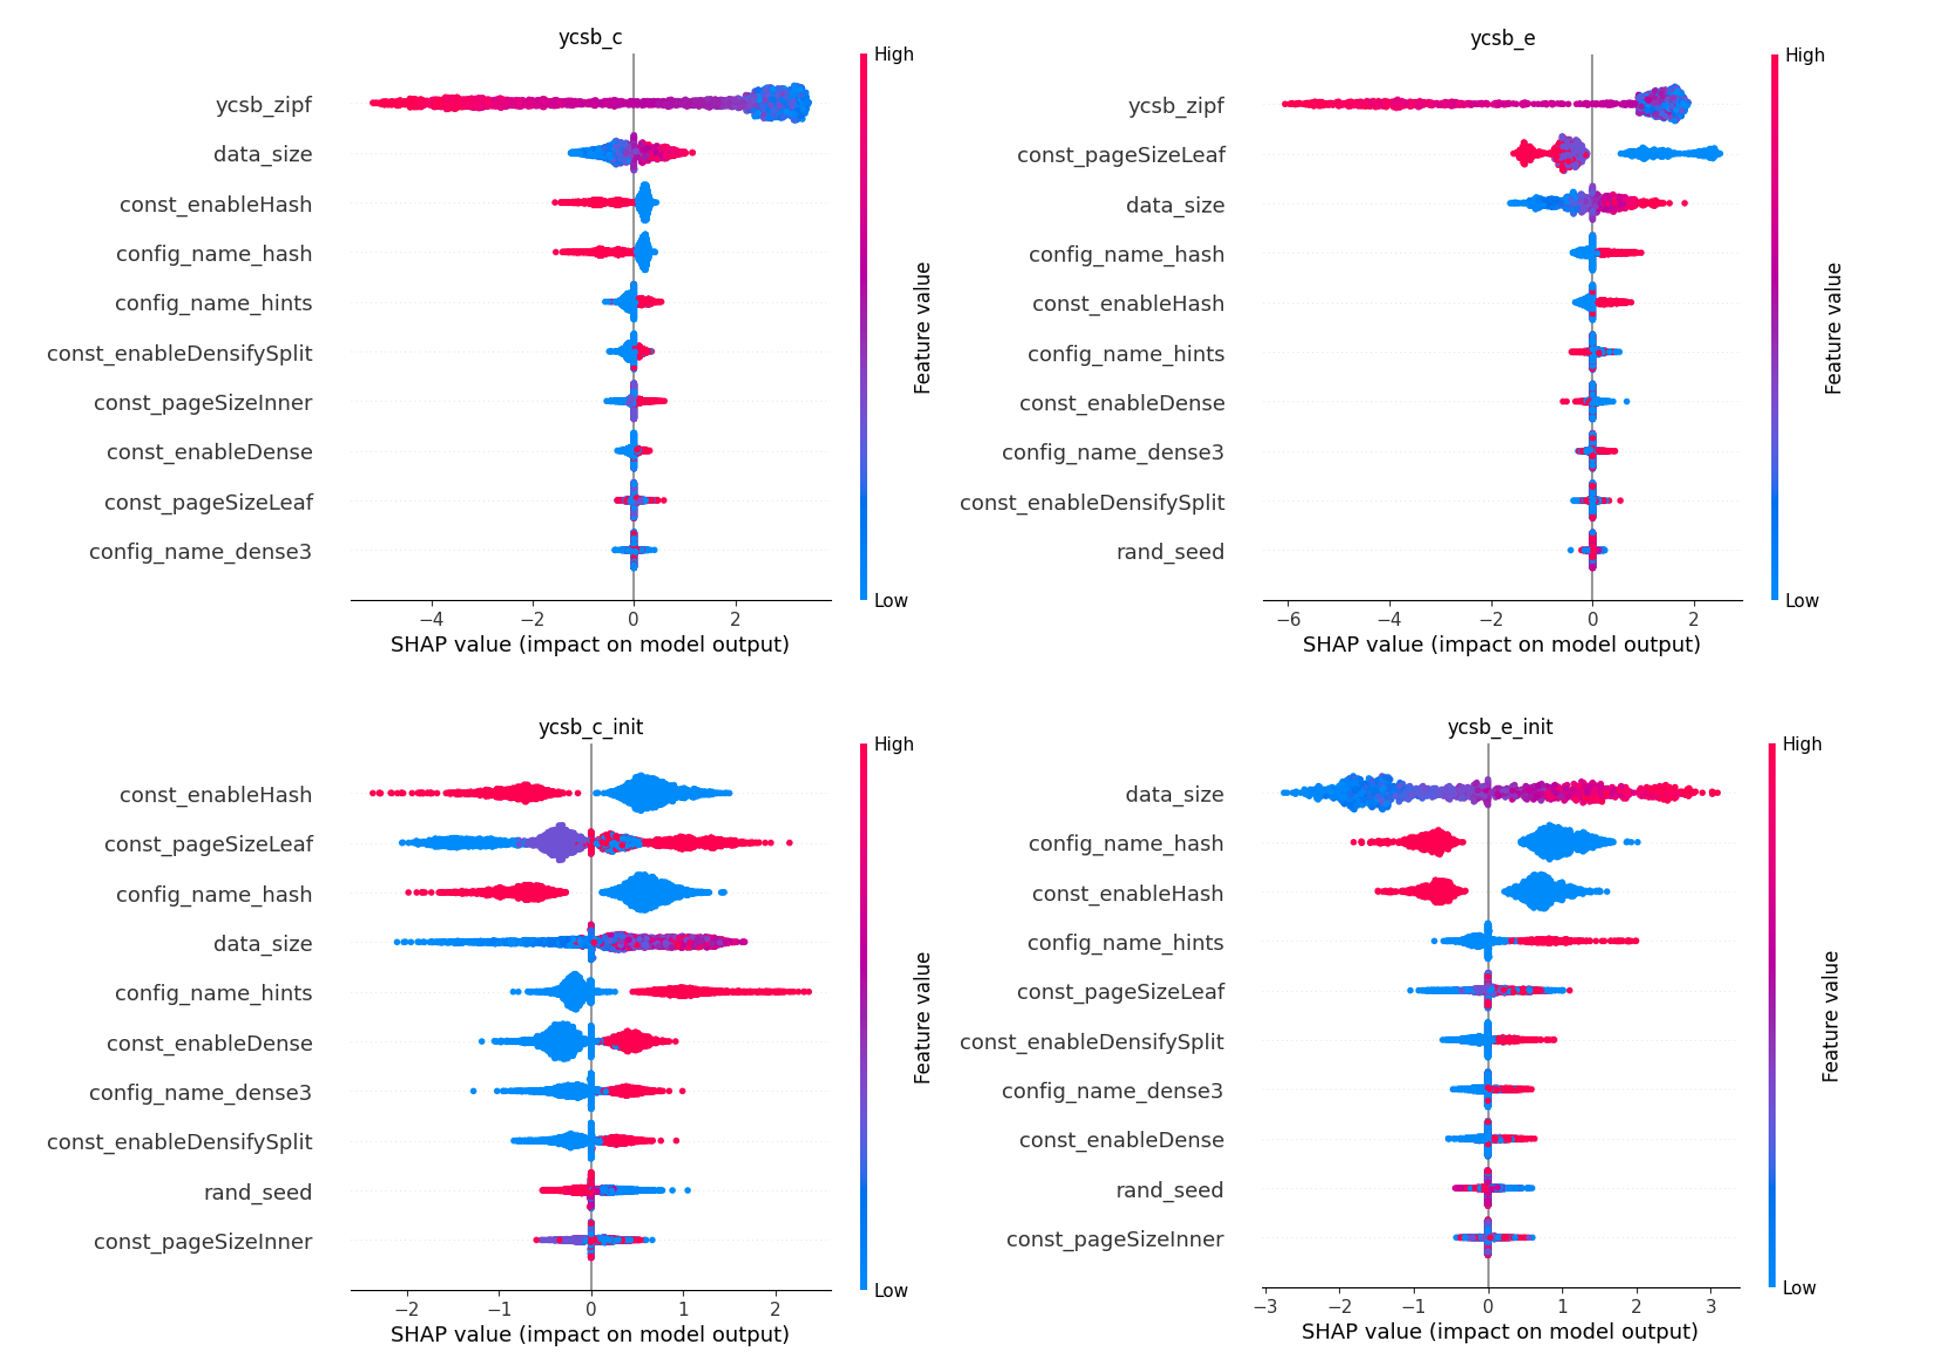
\includegraphics[width=0.9\textwidth]{images/shap_sum.png}
      \caption{Neural network SHAP summary plots per operation}
      \label{fig:shap_sum}
  \end{figure}
\\\\
Comparing the results between permutation feature importance plots and SHAP summary plots, the SHAP summary plots corroborate the conclusions drawn from the permutation feature importance plots. The SHAP summary plots, however, provide a few more insights. The colors in figure \ref{fig:shap_sum} indicate the plot relative feature value, with low values being blue and high values being red. These colors can then be compared with the Shapley values. For example, a cluster of blue dots for a feature on the positive side of the x-axis indicates that low values of the feature result in a higher target class, meaning a lower performance. 
\\\\
Based on this, it can be concluded that higher values of feature \textit{ycsb\_zipf} result in better performance for the operations \textit{ycsb\_c} and \textit{ycsb\_e}. The feature \textit{ycsb\_zipf} is generated randomly for each run between 0 and 1.5, with 0 meaning a normal distribution, 1 meaning a Zipfian distribution and above meaning even more skewed data. According to Claesen in \parencite{zipfdistr}, a Zipfian distribution indicates that fewer values are being accessed. Therefore, it can be interpreted that higher \textit{ycsb\_zipf} values indicate the cache can be better utilized, leading to better performance.
\\\\
For the feature \textit{data\_size} it is clearly visible at all operations that higher a smaller amount of data, leads to smaller trees and therefore a smaller class, meaning better performance. 
\\\\
Furthermore, for the initialization operations, one can notice that lower page sizes of leaf nodes result in better performance. This indicates that for the insertion operations benefit from lower leaf page sizes. Despite that, the \textit{ycsb\_e} figure could indicate a contradictory pattern, both patterns can be true. Considering that the \textit{ycsb\_e} consists of $95\%$ scan operations and only $5\%$ insertions, the scan operations outweigh the impact of the insertion operations. The scan operations, seem to benefit from higher leaf page sizes. This could be explained by the fact that higher leaf page sizes, lead to more consecutive values being stored in the same node and therefore during scan operations, fewer nodes need to be traversed. Insertion operations, on the other hand, might consider fewer values in a node more beneficial since it reduces the number of disk accesses required to write in a node. As a result, it can improve the performance of insertion operations, as disk I/O is often the bottleneck. This performance improvement seems to outweigh the drawback of having a higher depth and requiring more splitting operations. 

\section{Regression Models}
For regression models, the metrics have yielded the results depicted in figure \ref{fig:reg_mse} for metric MSE and figure \ref{fig:reg_r2} for metric $R^2$.
From these figures, one can conclude that the random forest model has yielded the best results in both metrics, with the exception of \textit{ycsb\_e\_init}, where the linear regression model performs better by a minimal margin.
\begin{figure}[H]
      \centering
      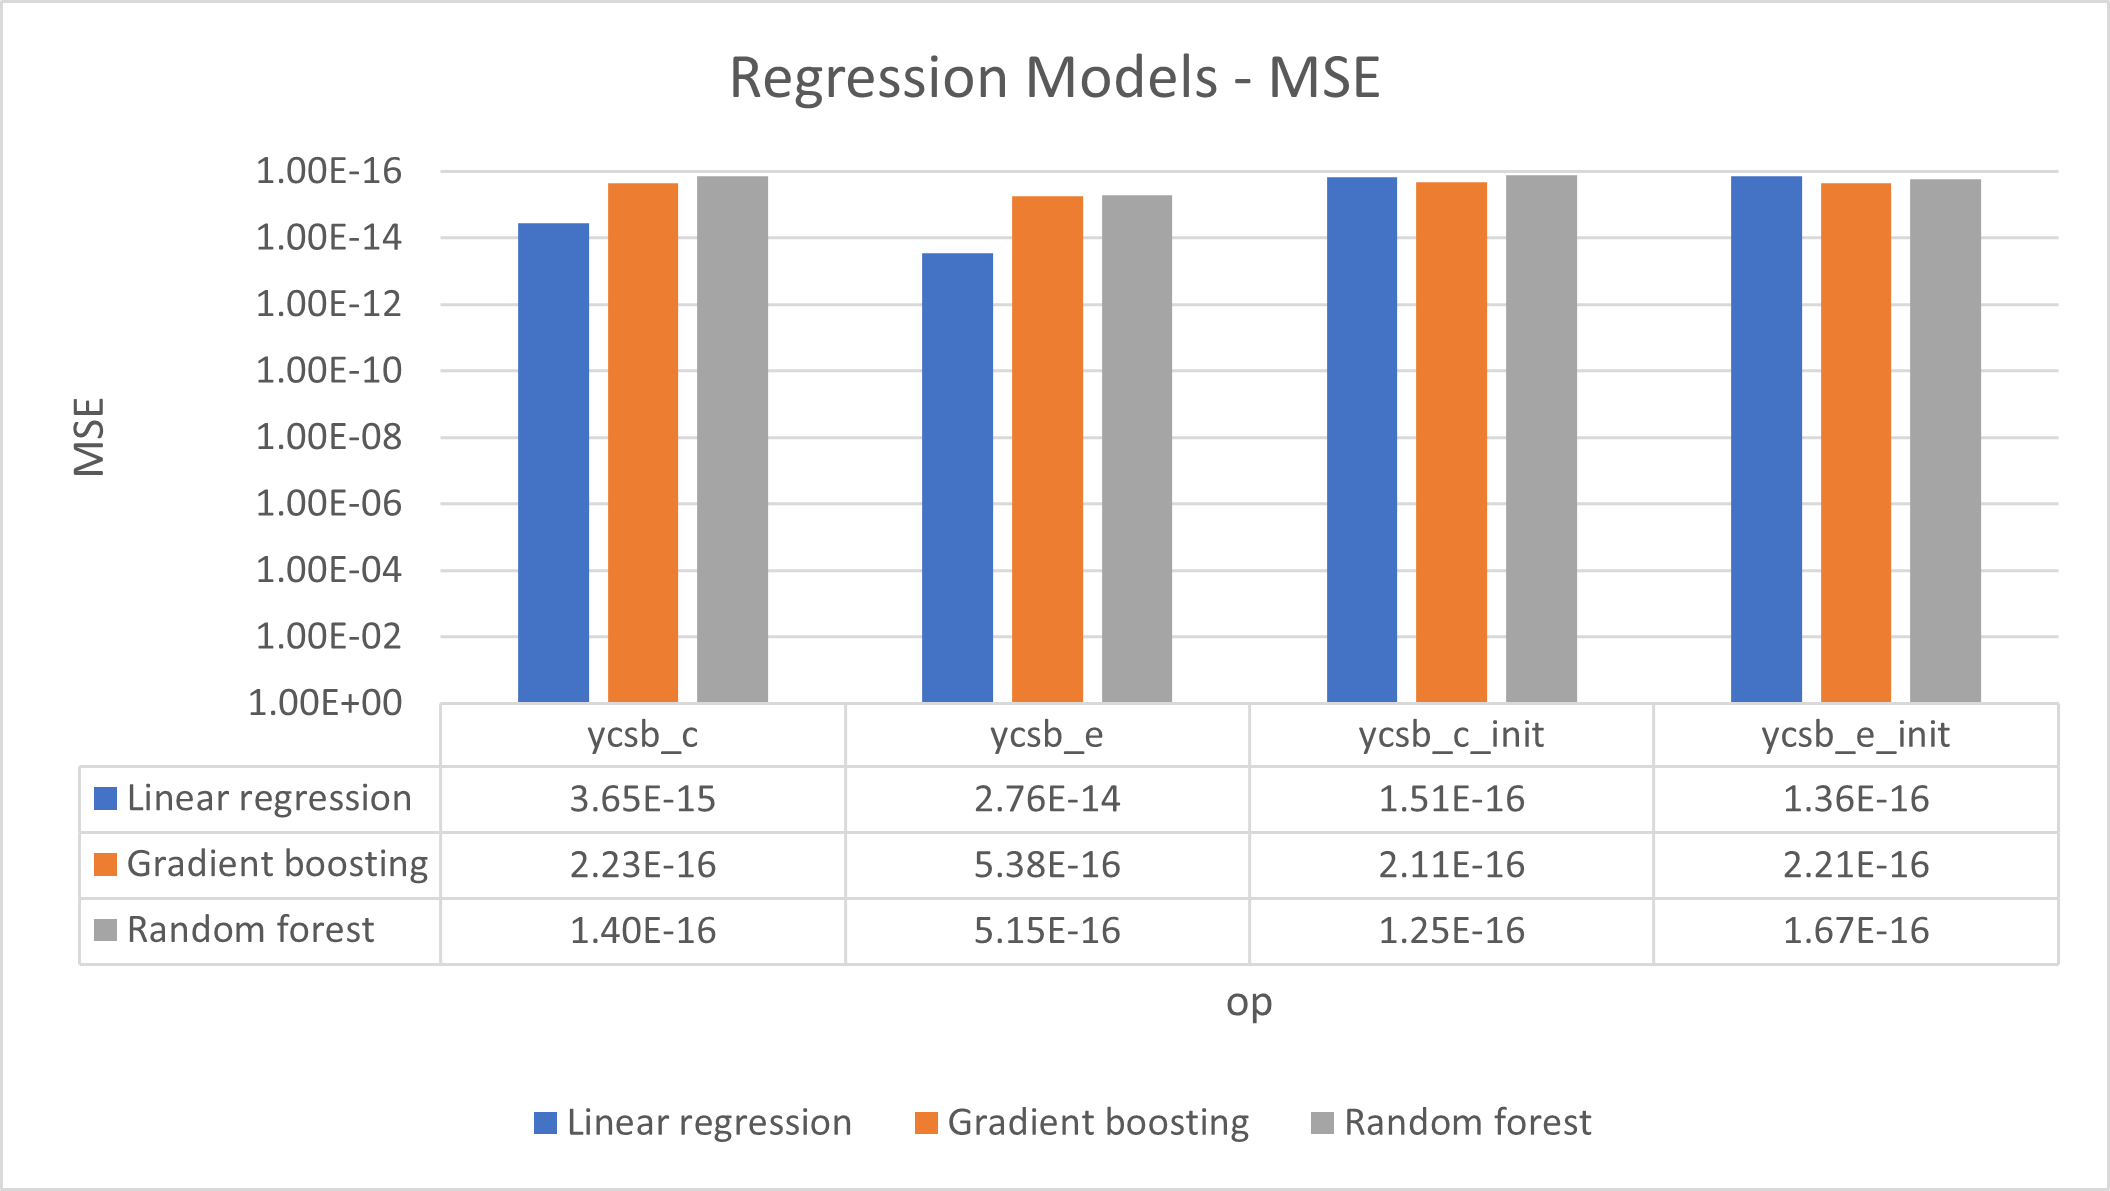
\includegraphics[width=0.8\textwidth]{images/reg_mse.png}
      \caption{Graph and data for MSE performance of regression models}
      \label{fig:reg_mse}
  \end{figure}
\begin{figure}[H]
      \centering
      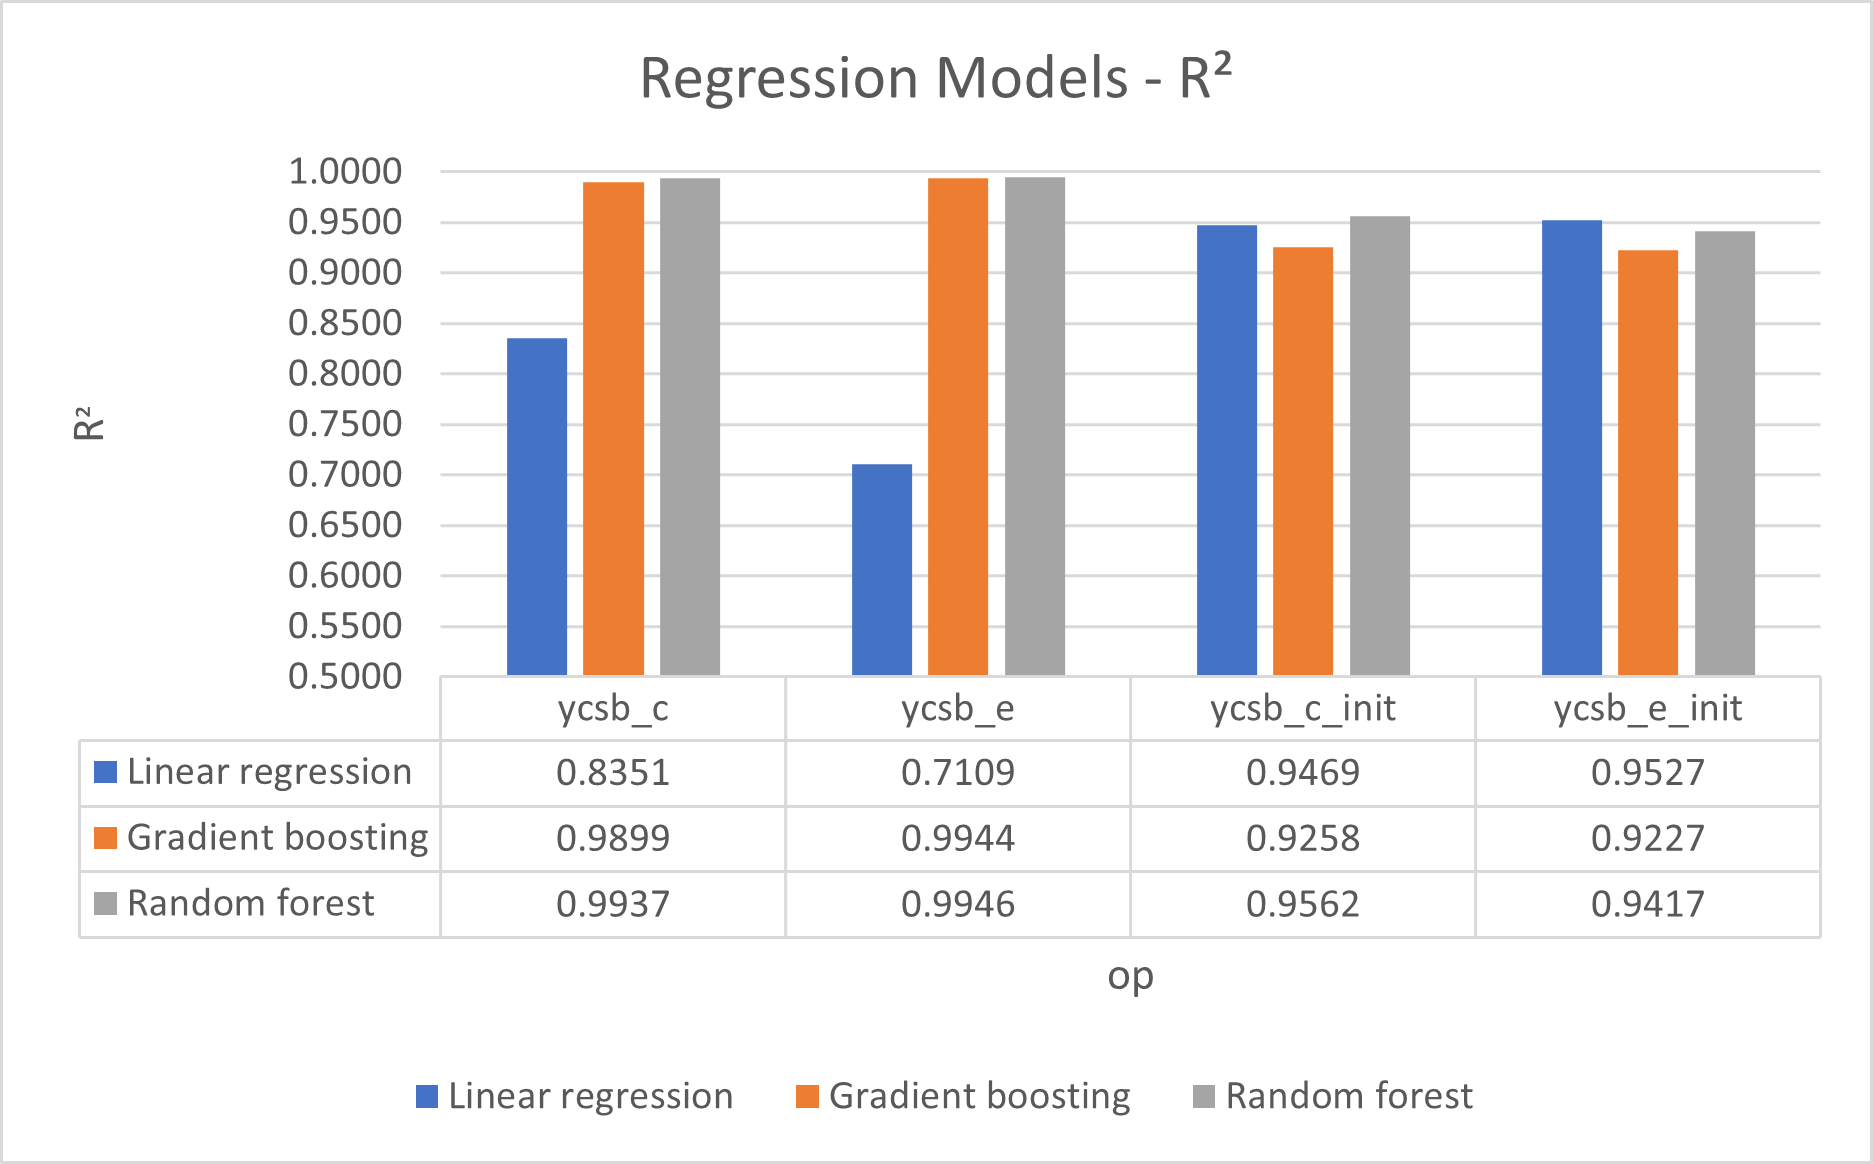
\includegraphics[width=0.8\textwidth]{images/reg_m2.png}
      \caption{Graph and data for $R^2$ performance of regression models}
      \label{fig:reg_r2}
  \end{figure}


\subsection{Permutation Feature Importance}
Producing insightful permutation feature importance plots has presented significant challenges, primarily stemming from the scale of the metrics and target feature. As a result, this particular step has been omitted from the scope of this thesis.\\

\subsection{SHAP Summary Plot}
Due to the scale of the target feature \textit{time}, the SHAP summary plots look differently, more clustered compared to the ones for classification. Nevertheless, similar outcomes can be deducted from the figure \ref{fig:shap_reg}. For example, the most important features remained the same, with only minor differences in order. Additionally, the same observations regarding features \textit{ycsb\_zipf}, \textit{const\_pageSizeLeaf} and \textit{data\_size} and their impact on the target feature can be made. However, due to the low interpretability caused by the scale of the target feature, the confidence for these statements is lower.


\begin{figure}[H]
      \centering
      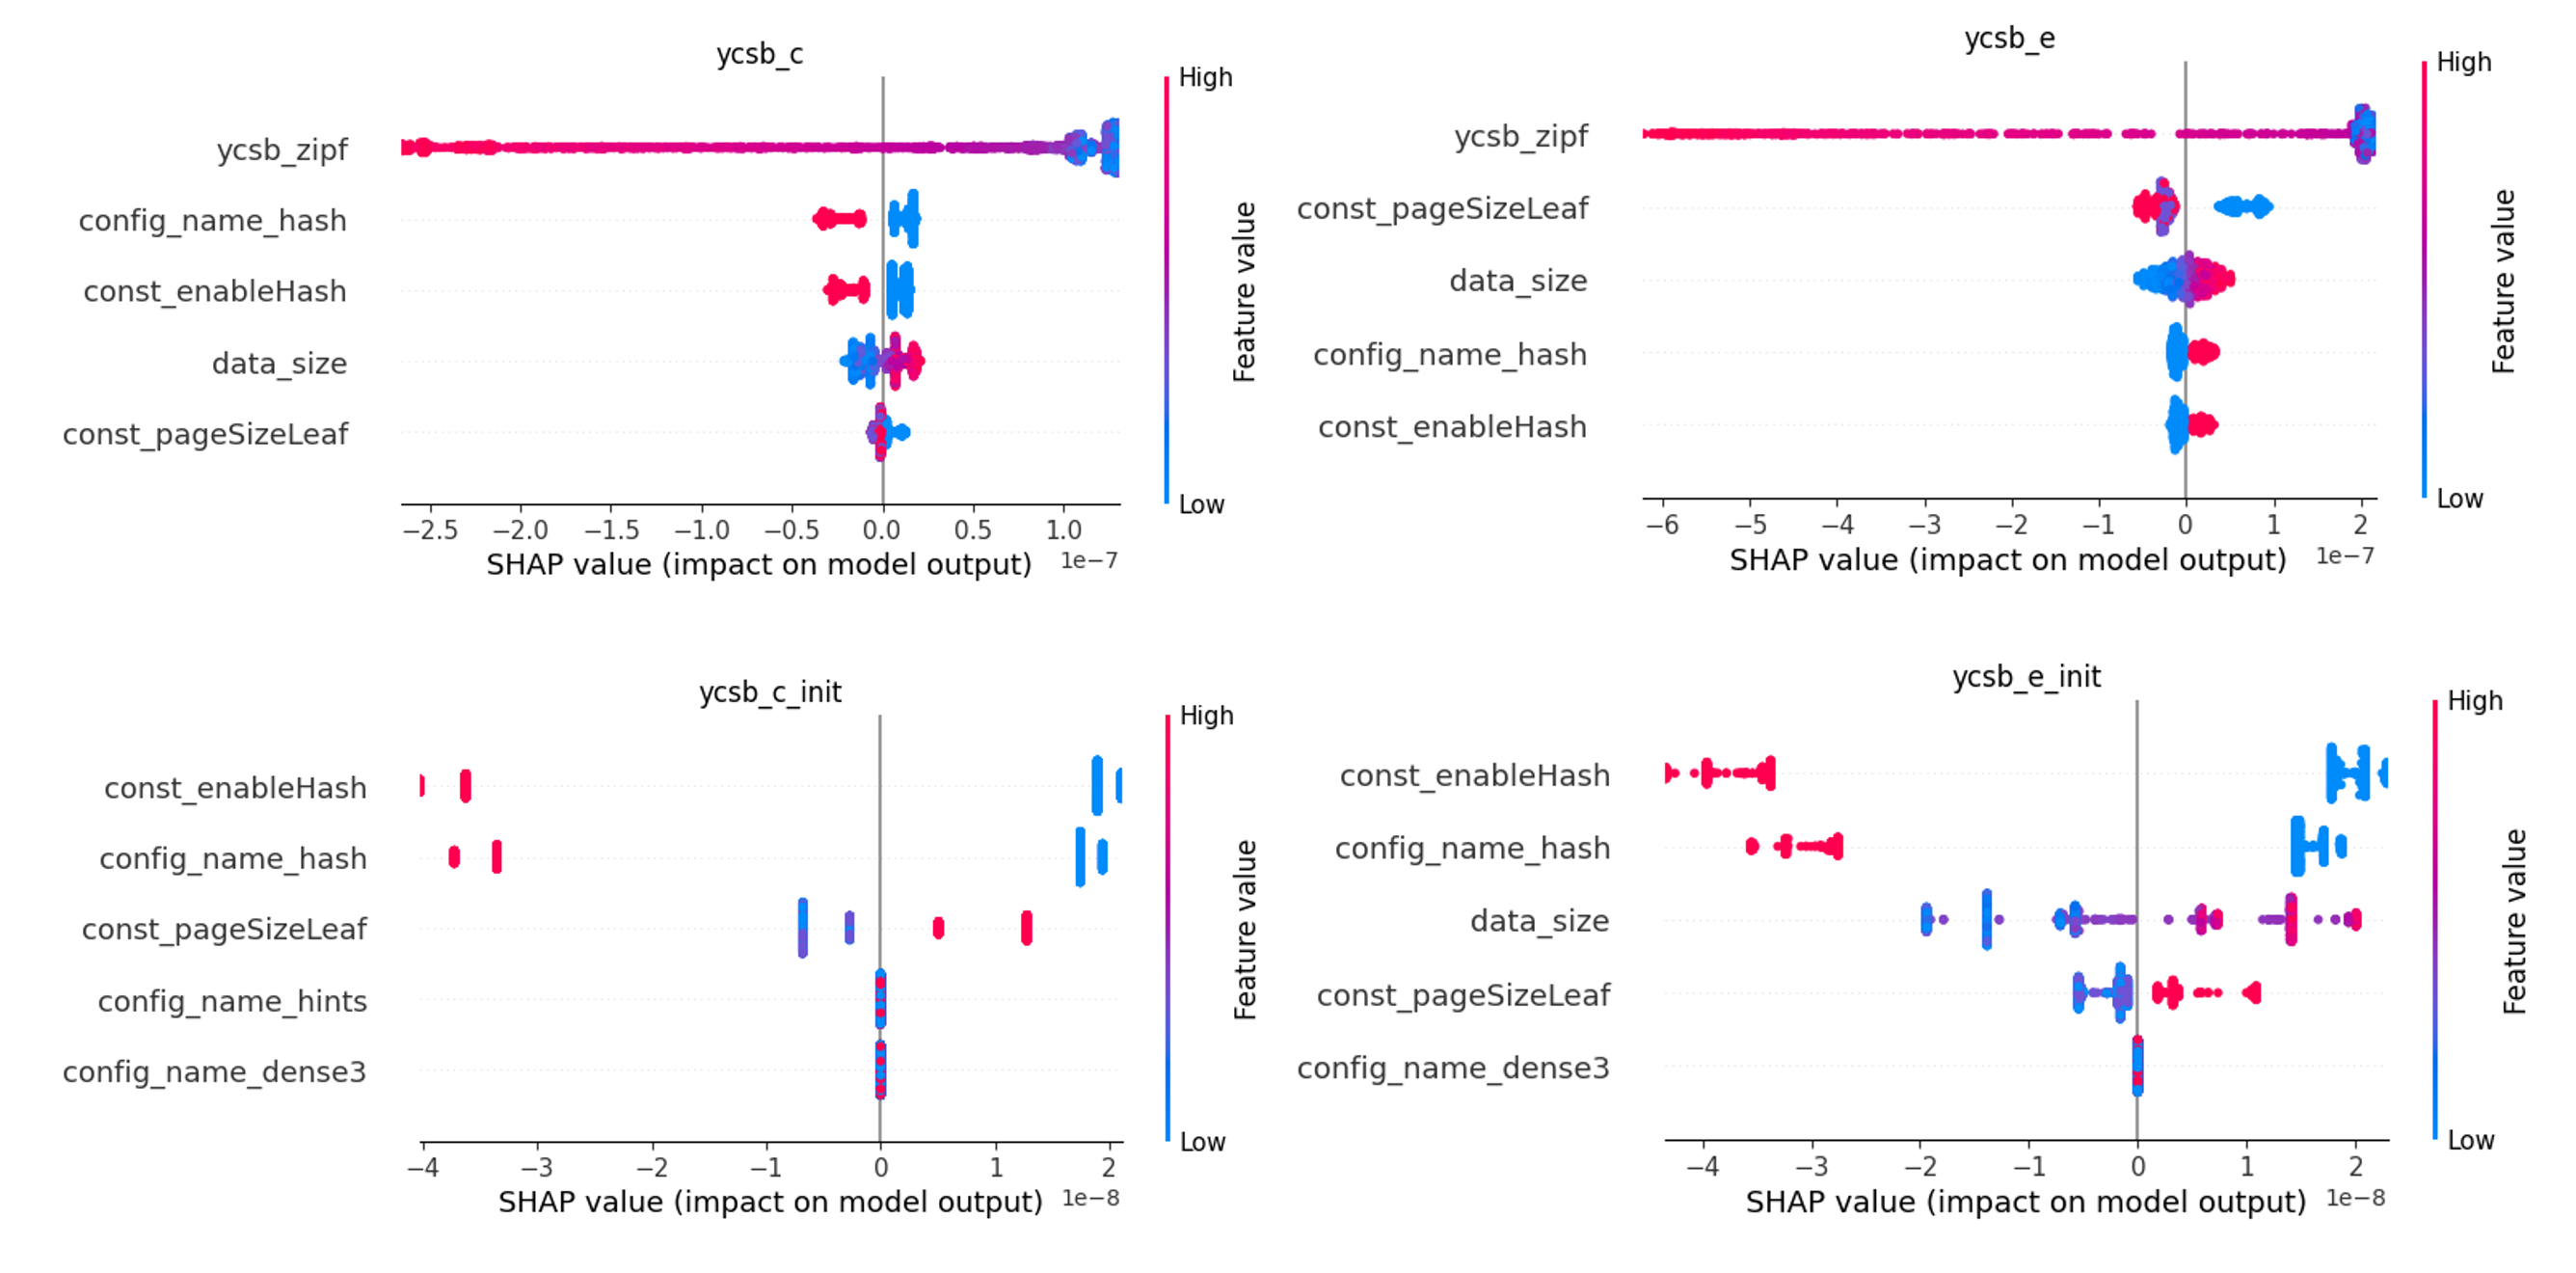
\includegraphics[width=0.95\textwidth]{images/shap_reg.png}
      \caption{Random forest SHAP summary plots per operation}
      \label{fig:shap_reg}
  \end{figure}




\section{Pattern recognition}
This section describes the results yielded by performing the Apriori algorithm and consequently the association rules mining algorithm. As described in chapter \ref{chapter:preprocessing} on preprocessing, the data used in this section is generated with a different data generation script than the one used for model training. The feature \textit{time}, is split into three buckets, as described, along with other necessary additional preprocessing steps, in section \ref{patternreg}. Bucket\_1 indicates the fastest times and therefore best performance.
\\\\
In the following results, the Apriori threshold has been set to $5\%$, and the association rules threshold for confidence to $40\%$. The result is then filtered to association rules, that are relevant to the performance. Additionally, to simplify the output, association rules that are redundant, by being majorly explained by a smaller antecedent, have been removed from the output. Furthermore, the consequent support is not displayed, since the buckets are split equally, meaning each has a support of close to $33\%$. Metrics not introduced in this thesis are also filtered out. 

\subsection{Association rules}

\textbf{ycsb\_c}:
As figure \ref{fig:pr_c} outlines, the major factor found for the purely read operation benchmark is feature \textit{data\_size}. Lower values for  \textit{data\_size} indicate better performance. Another notable result is that the biggest leaf page size for the benchmarking, 8192, tends to perform worst for this operation. 
\begin{figure}[h]
      \centering
      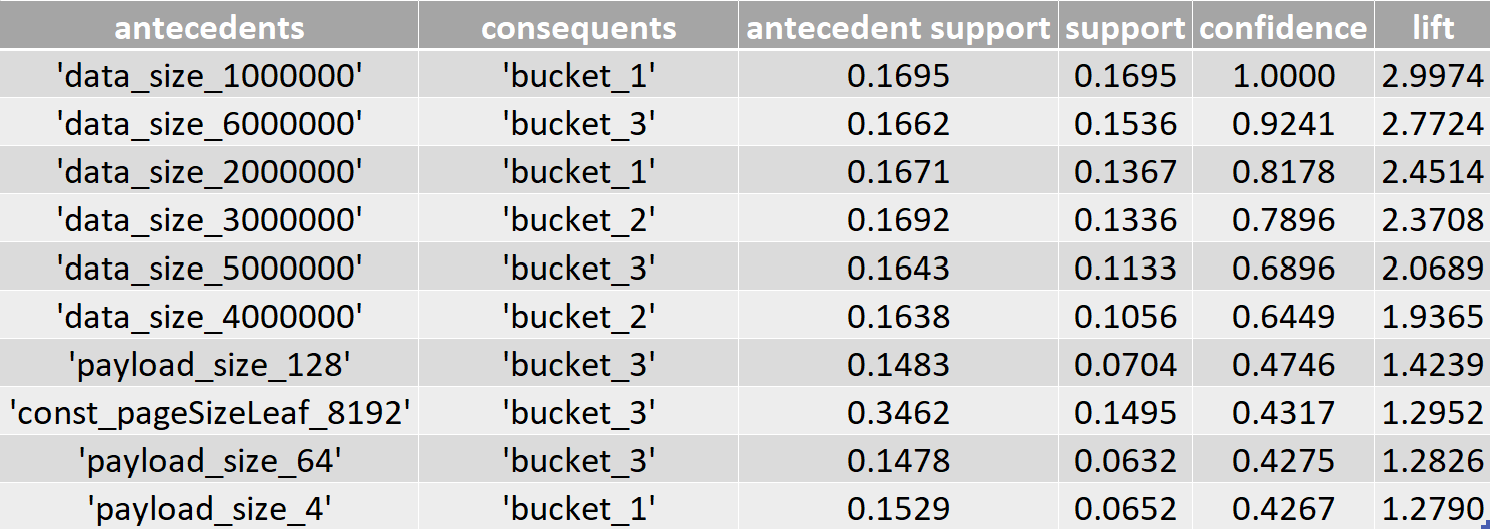
\includegraphics[width=0.6\textwidth]{images/pr_c.png}
      \caption{Association rules for \textit{ycsb\_c}}
      \label{fig:pr_c}
\end{figure}
\\\\
\textbf{ycsb\_e}:
For the operation \textit{ycsb\_e}, figure \ref{fig:pr_e} displays that the size of the payload is a decisive factor. For example, executions with payload size of 256, which occur about 10\% of the time in the dataset, end in the slowest bucket every time. Additionally, with the \textit{pageSizeLeaf} set to 2048, the executions mostly end up in the slowest two buckets, which considering that it is the lowest value in the dataset further underlines the findings from the previous section.
\begin{figure}[h]
      \centering
      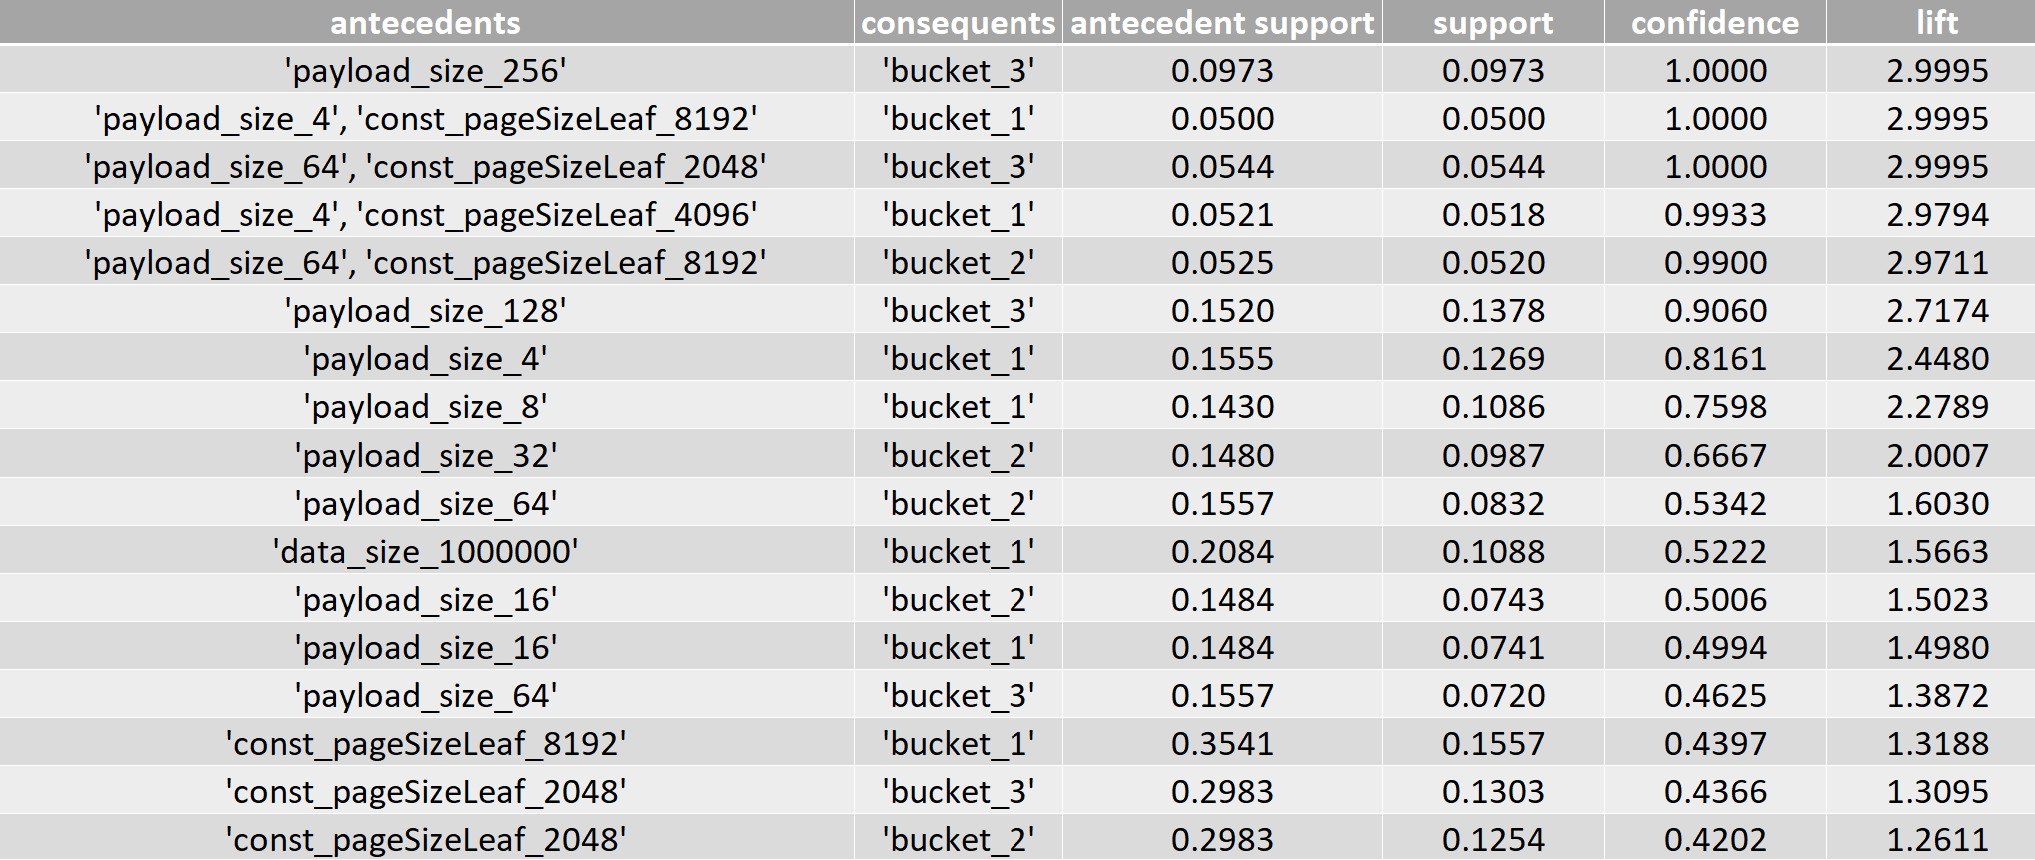
\includegraphics[width=0.6\textwidth]{images/pr_e.png}
      \caption{Association rules for \textit{ycsb\_e}}
      \label{fig:pr_e}
\end{figure}
\\\\
\textbf{ycsb\_c\_init}:
By looking at the figure \ref{fig:pr_c_init} one can observe a similar pattern, where the size of the payload and data can give a big indication, as to which of the three performance buckets the record belongs to. The pattern being that a high payload size indicates a slower performance. 
\begin{figure}[h]
      \centering
      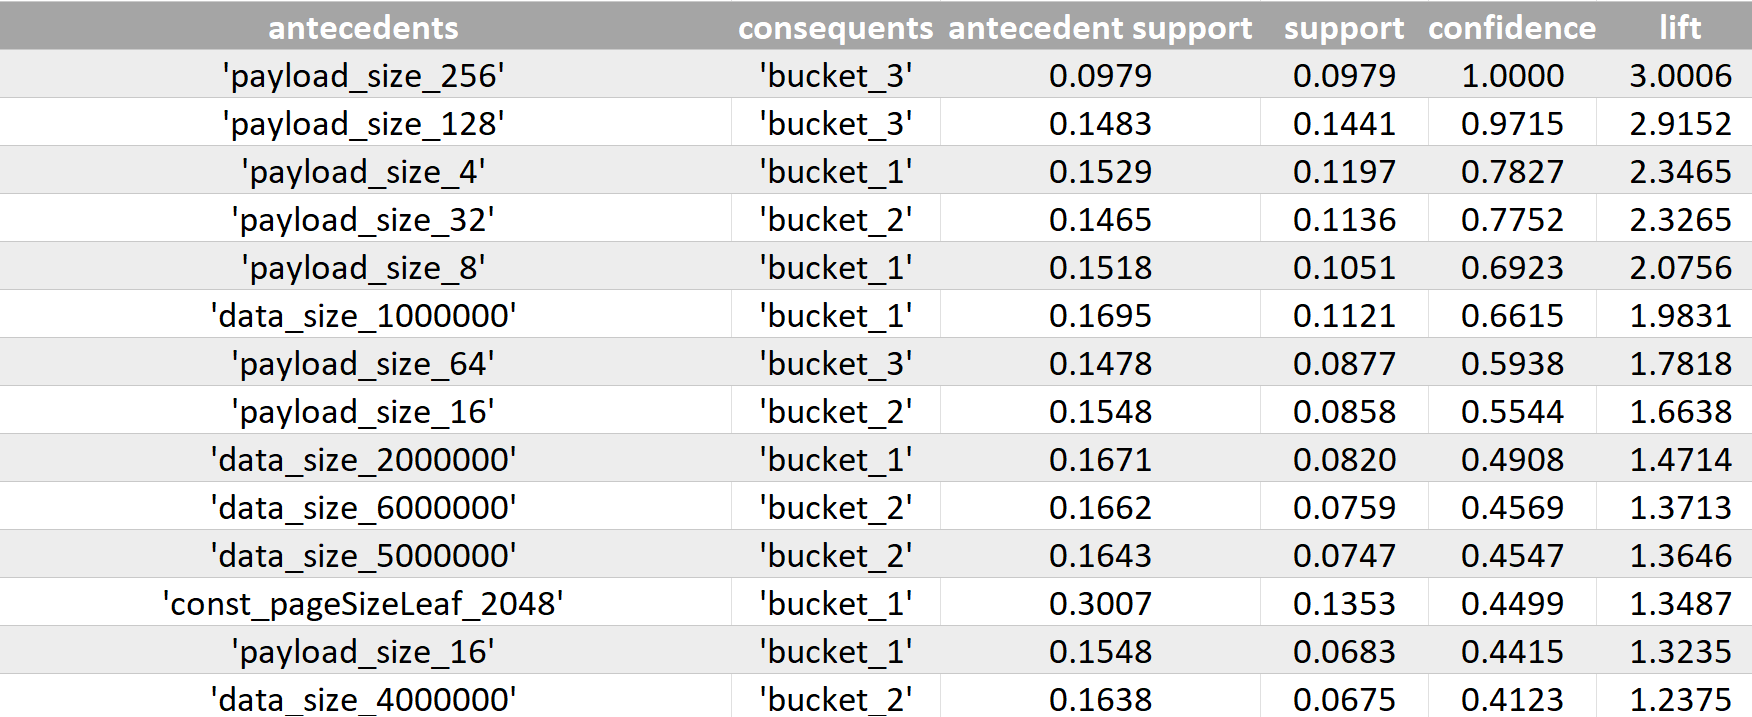
\includegraphics[width=0.6\textwidth]{images/pr_c_init.png}
      \caption{Association rules for \textit{ycsb\_c\_init}}
      \label{fig:pr_c_init}
\end{figure}
\\\\
\textbf{ycsb\_e\_init}:
The same observation as for operation \textit{ycsb\_c\_init} can be made for \textit{ycsb\_e\_init}. This is understandable, considering that these operations are very similar. The differences in values can be explained by the different scaling of feature \textit{time}. 
\begin{figure}[h]
      \centering
      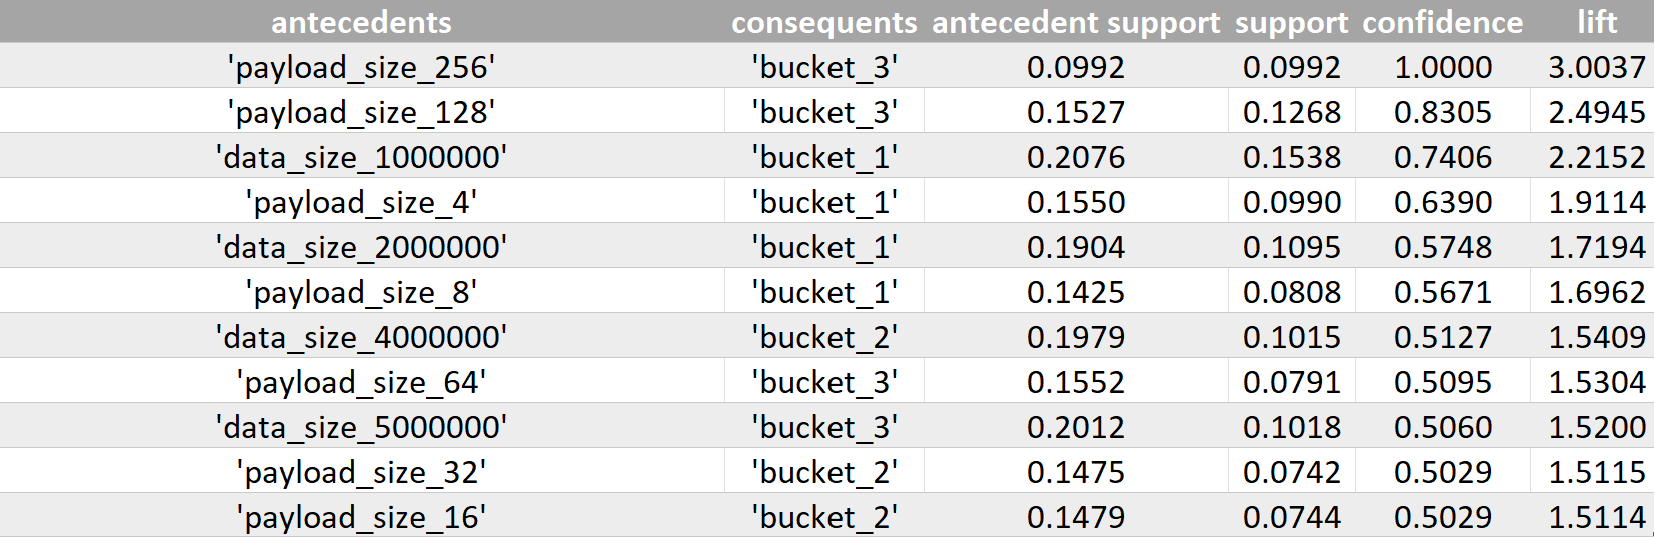
\includegraphics[width=0.6\textwidth]{images/pr_e_init.png}
      \caption{Association rules for \textit{ycsb\_e\_init}}
      \label{fig:pr_e_init}
\end{figure}


\subsection{Optimal page size of leaf nodes}
The methodology to generate heatmaps, based on regression models trained by the more discrete dataset, proved to be difficult. The output of the regression models, Random Forest and Gradient Boosting, as previous findings from the association rules indicate, greatly depends on the features \textit{payload\_size} and \textit{data\_size}. As a result, the various page sizes of leaf nodes received the same output based on features \textit{payload\_size} and \textit{data\_size}. Therefore, this methodology was not able to identify the optimal page size of leaf nodes. 
\\\\
Nevertheless, the heatmaps based on empirical means are generated and visualized in figure \ref{fig:heatmaps}.
\begin{figure}[h]
      \centering
      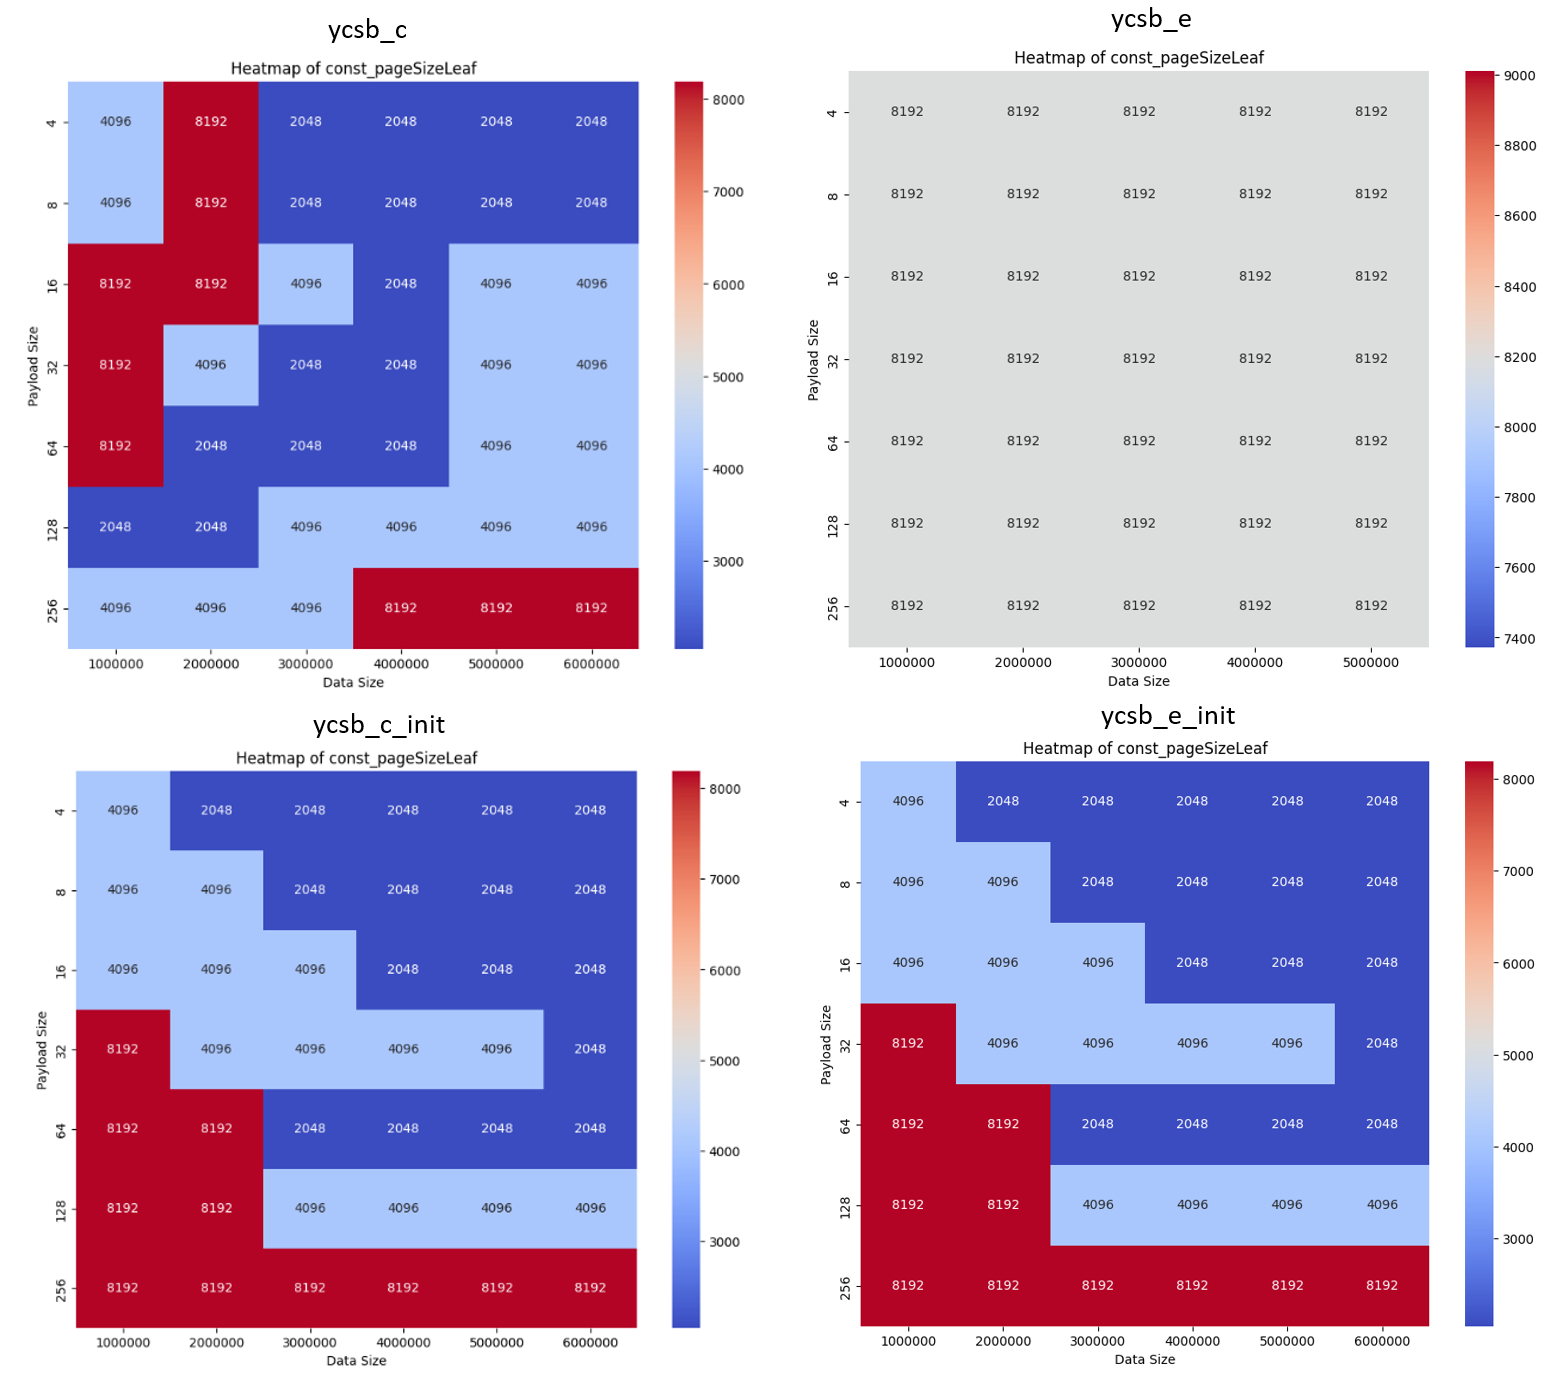
\includegraphics[width=0.95\textwidth]{images/heatmaps.png}
      \caption{Heatmaps per operation based on empirical mean}
      \label{fig:heatmaps}
\end{figure}
\\\\
The findings of operation \textit{ycsb\_e} indicate the high importance of big page sizes for scan operations. The page size 8192 is the highest in the data set, meaning that potentially a higher page size might be optimal. Operations {ycsb\_c\_init} and {ycsb\_e\_init} generated the same behavior, which is expected due to their similar nature. The pattern seems to indicate that during the insertion operations, higher sizes of the payload prefer higher page sizes, however, the bigger the size of the dataset, lower page sizes are preferred. These findings should be interpreted with caution, as the optimal page sizes generally result in only an $1-3\%$ improvement compared to the next best page size. Given that the values of the feature \textit{time} are in the order of magnitude of hundreds of nanoseconds  ($10^{-7}$ seconds), an $1-3\%$ improvement may not be considered substantial. Consequently, the heatmap for operation \textit{ycsb\_c} is not further analyzed. 
\chapter{Conclusion and Future Work }\label{chapter:summary}
This thesis explored the use of \ac{ML} models to analyze behavior of B+ trees with different optimizations and configurations. The aim of this thesis was to find insights into how one can improve the performance of B+ trees.
\\\\
The methodology used in this thesis explored multiple ways of getting the desired insights. Firstly, two datasets were created, by running a benchmarking program many times with a varying B+ tree configurations, and measuring the performance of each run. These datasets were then preprocessed to fit the desired structures of the used algorithms.
\\\\
The initial, statistical analysis brought meaningful insights into which features can and can not be used for trying to identify patterns between inputs and outputs.
\\\\
The main approach of this thesis was to train classification models on the dataset and identify, using \ac{XAI} on the best performing model, which inputs, impact the performance and how. The best performing model for the dataset was a neural network classifier, which by using on SHAP summary plots indicated the most influential parameters for performance. The skewness of the data together with the size of the data seem to impact the performance the most. For inserting and scan operations, the page size of leaf nodes can impact the performance as well. This indicates that an implementation of adaptive B+ trees, could potentially further improve performance of the data structure.
\\\\
The second approach was to use regression models, which managed to get good results in terms of their $R^2$ metrics. However, using \ac{XAI} algorithms on the models and getting insights from those proved to be mode difficult due to the scale of the feature \textit{time}. Nevertheless, some insights gained from the first approach, were further supported.
\\\\
Another approach was to use data mining pattern recognition techniques, to find patterns in the data. The association rule mining algorithm was used on a dataset, which has more discrete feature values, with fewer variations. This approach ultimately confirmed the claim that a bigger size of payload or data, impacts the performance negatively. Retrospectively, one could generate the dataset by not varying these parameters, and instead focus more on varying the page size of the leaf node and other optimizations. This way, one could identify more relevant patterns for an adaptive B+ tree. 
\\\\
Lastly, it was attempted to take train regression models on the dataset for pattern recognition techniques and generate heatmaps to create an overview of which payload and data size combination benefit from which page size of leaf nodes the most. This approach, however, failed due to the models not assigning enough importance to the page size. Nevertheless, a heatmap based on the empirical means and not the regression models was generated and discussed.
\\\\
One key observation, outside the scope of B+ trees, is that using \ac{XAI} on \ac{ML} models is a viable way to gain valuable insights into a dataset.
\\\\
In future works, this thesis could be expanded to use other types of data, instead of restricting itself to urls. Additionally, more parameters could be varied, and a bigger dataset created, to yield more confident results. Using the approaches demonstrated in this thesis, one could potentially identify more helpful patterns.

% % !TeX root = ../main.tex
% Add the above to each chapter to make compiling the PDF easier in some editors.

\chapter{Introduction}\label{chapter:introduction}

\section{Section}
Citation test~\parencite{latex}.

Acronyms must be added in \texttt{main.tex} and are referenced using macros. The first occurrence is automatically replaced with the long version of the acronym, while all subsequent usages use the abbreviation.

E.g. \texttt{\textbackslash ac\{TUM\}, \textbackslash ac\{TUM\}} $\Rightarrow$ \ac{TUM}, \ac{TUM}

For more details, see the documentation of the \texttt{acronym} package\footnote{\url{https://ctan.org/pkg/acronym}}.
\subsection{Subsection}

See~\autoref{tab:sample}, \autoref{fig:sample-drawing}, \autoref{fig:sample-plot}, \autoref{fig:sample-listing}.

\begin{table}[htpb]
  \caption[Example table]{An example for a simple table.}\label{tab:sample}
  \centering
  \begin{tabular}{l l l l}
    \toprule
      A & B & C & D \\
    \midrule
      1 & 2 & 1 & 2 \\
      2 & 3 & 2 & 3 \\
    \bottomrule
  \end{tabular}
\end{table}

\begin{figure}[htpb]
  \centering
  % This should probably go into a file in figures/
  \begin{tikzpicture}[node distance=3cm]
    \node (R0) {$R_1$};
    \node (R1) [right of=R0] {$R_2$};
    \node (R2) [below of=R1] {$R_4$};
    \node (R3) [below of=R0] {$R_3$};
    \node (R4) [right of=R1] {$R_5$};

    \path[every node]
      (R0) edge (R1)
      (R0) edge (R3)
      (R3) edge (R2)
      (R2) edge (R1)
      (R1) edge (R4);
  \end{tikzpicture}
  \caption[Example drawing]{An example for a simple drawing.}\label{fig:sample-drawing}
\end{figure}

\begin{figure}[htpb]
  \centering

  \pgfplotstableset{col sep=&, row sep=\\}
  % This should probably go into a file in data/
  \pgfplotstableread{
    a & b    \\
    1 & 1000 \\
    2 & 1500 \\
    3 & 1600 \\
  }\exampleA
  \pgfplotstableread{
    a & b    \\
    1 & 1200 \\
    2 & 800 \\
    3 & 1400 \\
  }\exampleB
  % This should probably go into a file in figures/
  \begin{tikzpicture}
    \begin{axis}[
        ymin=0,
        legend style={legend pos=south east},
        grid,
        thick,
        ylabel=Y,
        xlabel=X
      ]
      \addplot table[x=a, y=b]{\exampleA};
      \addlegendentry{Example A};
      \addplot table[x=a, y=b]{\exampleB};
      \addlegendentry{Example B};
    \end{axis}
  \end{tikzpicture}
  \caption[Example plot]{An example for a simple plot.}\label{fig:sample-plot}
\end{figure}

\begin{figure}[htpb]
  \centering
  \begin{tabular}{c}
  \begin{lstlisting}[language=SQL]
    SELECT * FROM tbl WHERE tbl.str = "str"
  \end{lstlisting}
  \end{tabular}
  \caption[Example listing]{An example for a source code listing.}\label{fig:sample-listing}
\end{figure}





% TODO: add more chapters here

\appendix{}

\microtypesetup{protrusion=false}

\addchap{Abbreviations}

\begin{acronym}
	\itemsep-.25\baselineskip
	\acro{XAI}[XAI]{Explainable Artificial Intelligence}
	% TODO: add acronyms
\end{acronym}
\begin{acronym}
	\itemsep-.25\baselineskip
	\acro{ML}[ML]{Machine Learning}
\end{acronym}
\begin{acronym}
	\itemsep-.25\baselineskip
	\acro{ycsb}[YCSB]{Yahoo! Cloud Serving Benchmark}
\end{acronym}


\listoffigures{}
\listoftables{}
\microtypesetup{protrusion=true}

\printbibliography{}

\end{document}
